\documentclass[12pt,a4paper]{article}
\usepackage{geometry}
\usepackage{graphicx}
\usepackage{fancyhdr}
\usepackage{titlesec}
\usepackage{titletoc}
\usepackage{ctex}
\usepackage{tocloft}
\usepackage{setspace}
\usepackage{float}
\usepackage{amsmath}
% 页面设置
\linespread{1.5}\selectfont    %1.5倍行距
\geometry{
    left=2.5cm,    % 左边距
    right=2.5cm,   % 右边距
    top=1cm,       % 上边距(页眉到页顶的距离)
    bottom=3cm,    % 下边距(页脚到页底的距离)
    % 可选:设置纸张大小(默认是a4paper,可省略)
    paper=a4paper,
    % 可选:是否包含页眉页脚在边距内(默认不包含)
    includeheadfoot=true
}
\setlength{\headheight}{76pt}
\pagestyle{fancy}
\fancyhf{}
\lhead{
\includegraphics[width=0.3\textwidth]{logo2.png}}
\cfoot{\thepage}

% 标题格式设置
\titleformat{\section}[hang]{\Large\bfseries}{\thesection}{1em}{}
\titleformat{\subsection}[hang]{\large\bfseries}{\thesubsection}{1em}{}

% 目录格式设置
\setcounter{tocdepth}{2}
\titlecontents{section}[1em]{\addvspace{0.5em}\bfseries}{\thecontentslabel\ }{}{\titlerule*[0.5pc]{.}\contentspage}
\titlecontents{subsection}[4em]{\addvspace{0.3em}}{\thecontentslabel\ }{}{\titlerule*[0.5pc]{.}\contentspage}
\titlecontents{subsubsection}[6em]{\addvspace{0.3em}}{\thecontentslabel\ }{}{\titlerule*[0.5pc]{.}\contentspage}
\renewcommand{\cfttoctitlefont}{\hfill\Large\bfseries} % 标题左侧添加空白填充(向右推)
\renewcommand{\cftaftertoctitle}{\hfill}
\setlength{\cftbeforetoctitleskip}{2cm}

\begin{document}

% 封面页
\begin{titlepage}
    \centering
    \vspace*{0.5cm}
    
    
\includegraphics[width=0.95\textwidth]{logo1.png}\\[3cm] % 替换为学校Logo
    
    {\fontsize{30}{32}\selectfont\bfseries 数据结构课程设计}\\[2cm]
    {\large 姓名: 陆彦翔}\\[1cm]
    {\large 学号: 2352975}\\[1cm]
    {\large 专业: 信息安全}\\[1cm]
    
    {\large 日期: 2025年8月}\\[1cm] % 自动生成当前日期
\end{titlepage}

% 目录页
\newpage
\tableofcontents


% 正文内容示例(一级和二级标题)
\newpage
\section{第一部分:算法实现}
\subsection{实现内容概述}
本部分内容旨在实现二叉树相关功能,并通过一个可视化界面实现用户交互。具体实现内容如下:

1.通过先序序列建立一颗二叉树;

2.实现先序、中序和后序遍历,并输出遍历序列;

3.递归统计二叉树中的叶子结点个数并输出;

4.分别进行先序、中序和后序线索化;

5.实现先序线索树和中序线索树的遍历(无需栈/递归),输出遍历序列;

6.以树形格式可视化输出原二叉树结构,同时输出线索化后的结点信息(包括数据、指针类型及线索目标)

\subsection{软件介绍}
\subsubsection{整体界面介绍}
\begin{figure}[H]
    \centering
    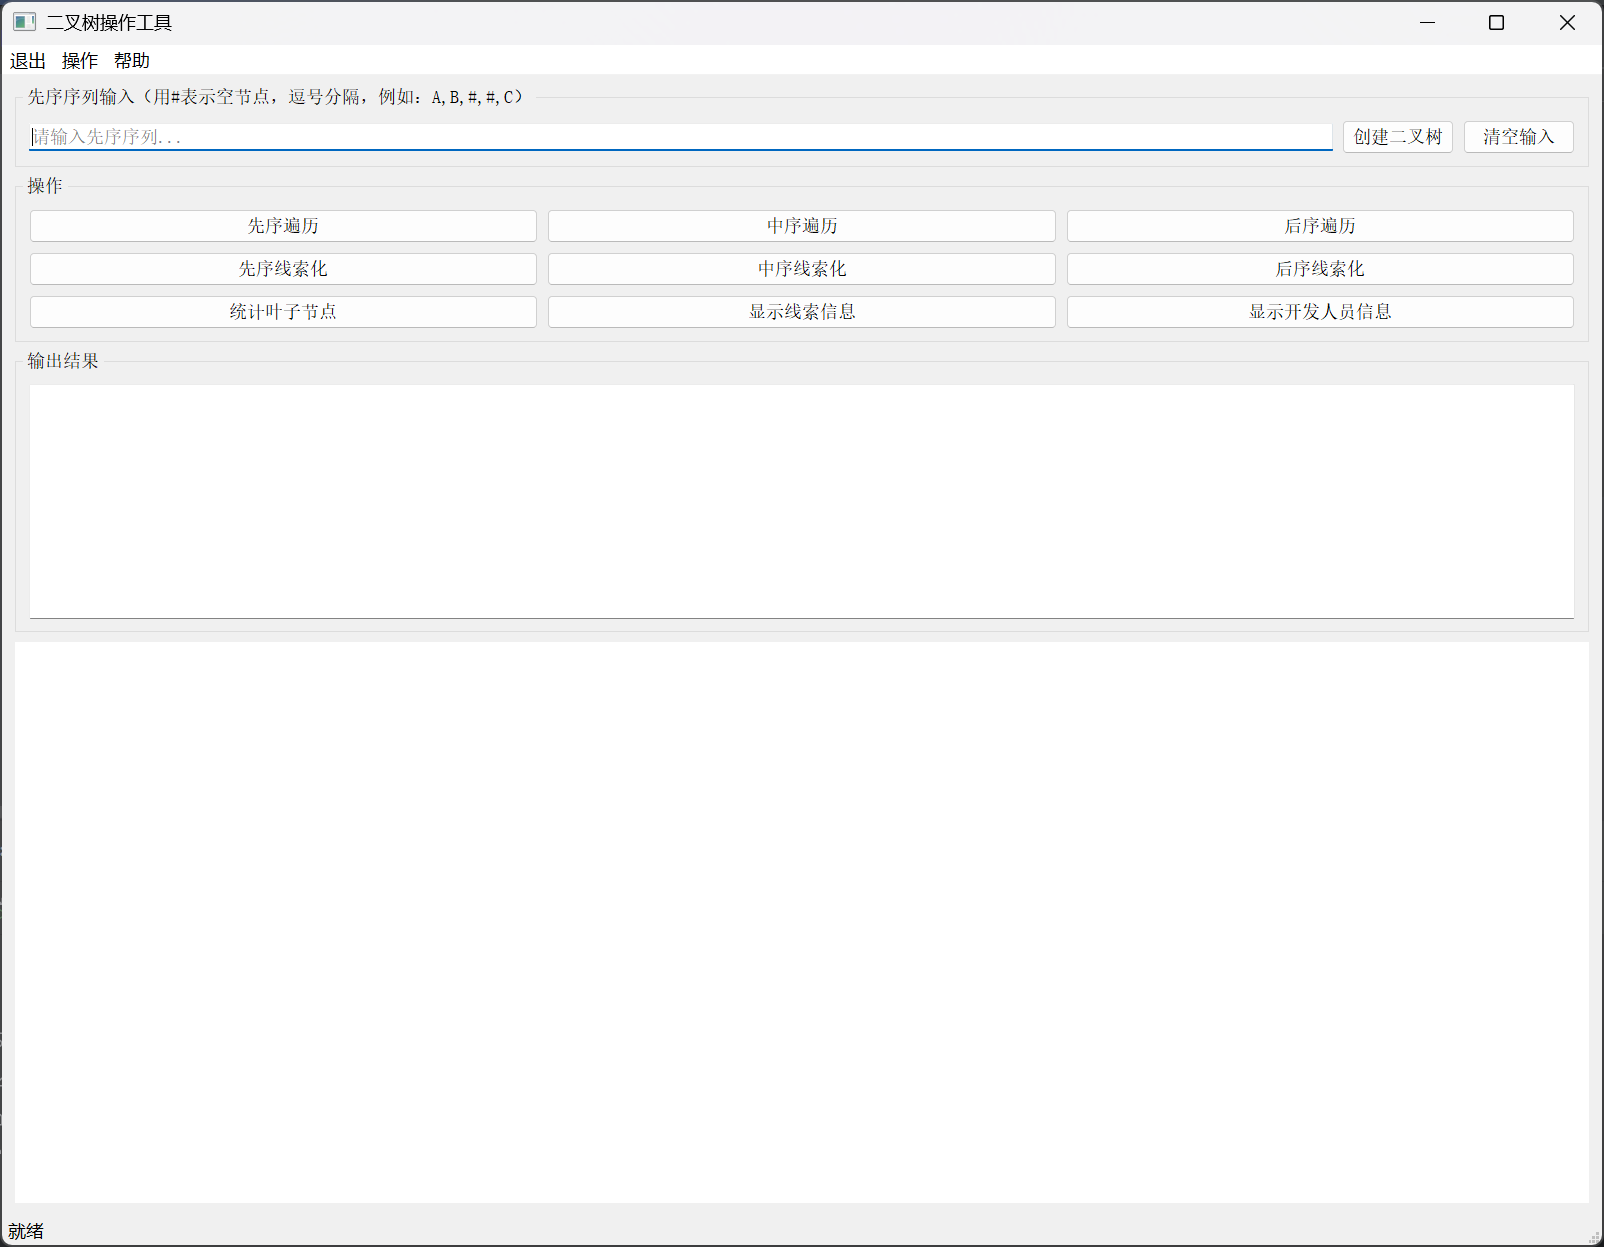
\includegraphics[width=0.5\textwidth]{pt1-1.png}
    \caption{整体界面}
\end{figure}
整个界面大体由五个部分组成:菜单栏,二叉树序列构建框,操作按钮,输出结果提示框以及画布。
\begin{figure}[H]
    \centering
    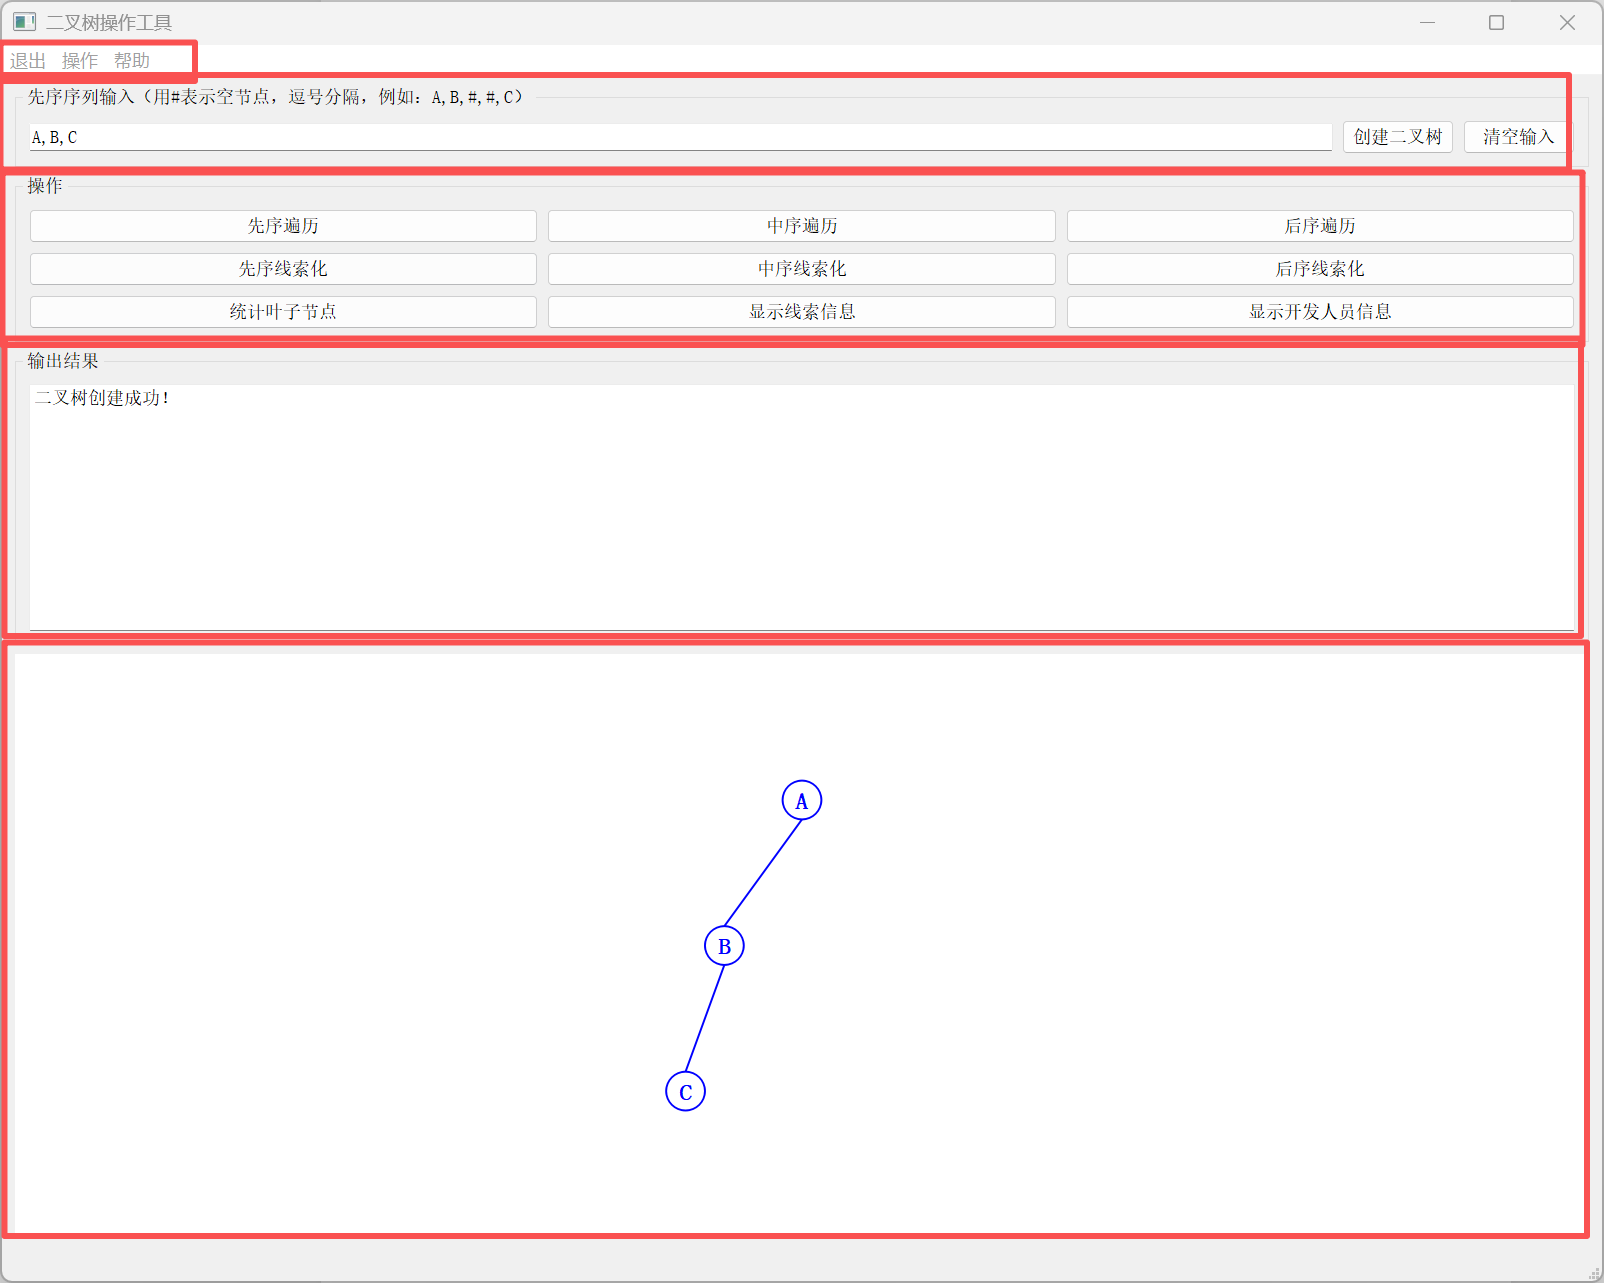
\includegraphics[width=0.5\textwidth]{pt1-2.png}
    \caption{界面五大部分}
\end{figure}
用户可以在菜单栏中选择退出程序,或者执行与操作栏中九个操作内容相同的操作(即此处只是增加了一个操作方式,内容没有改变)。同时这里还设置了一个操作帮助按钮,如果点击操作帮助,那么就会在输出框中出现操作相关提示。
\begin{figure}[H]
    \centering
    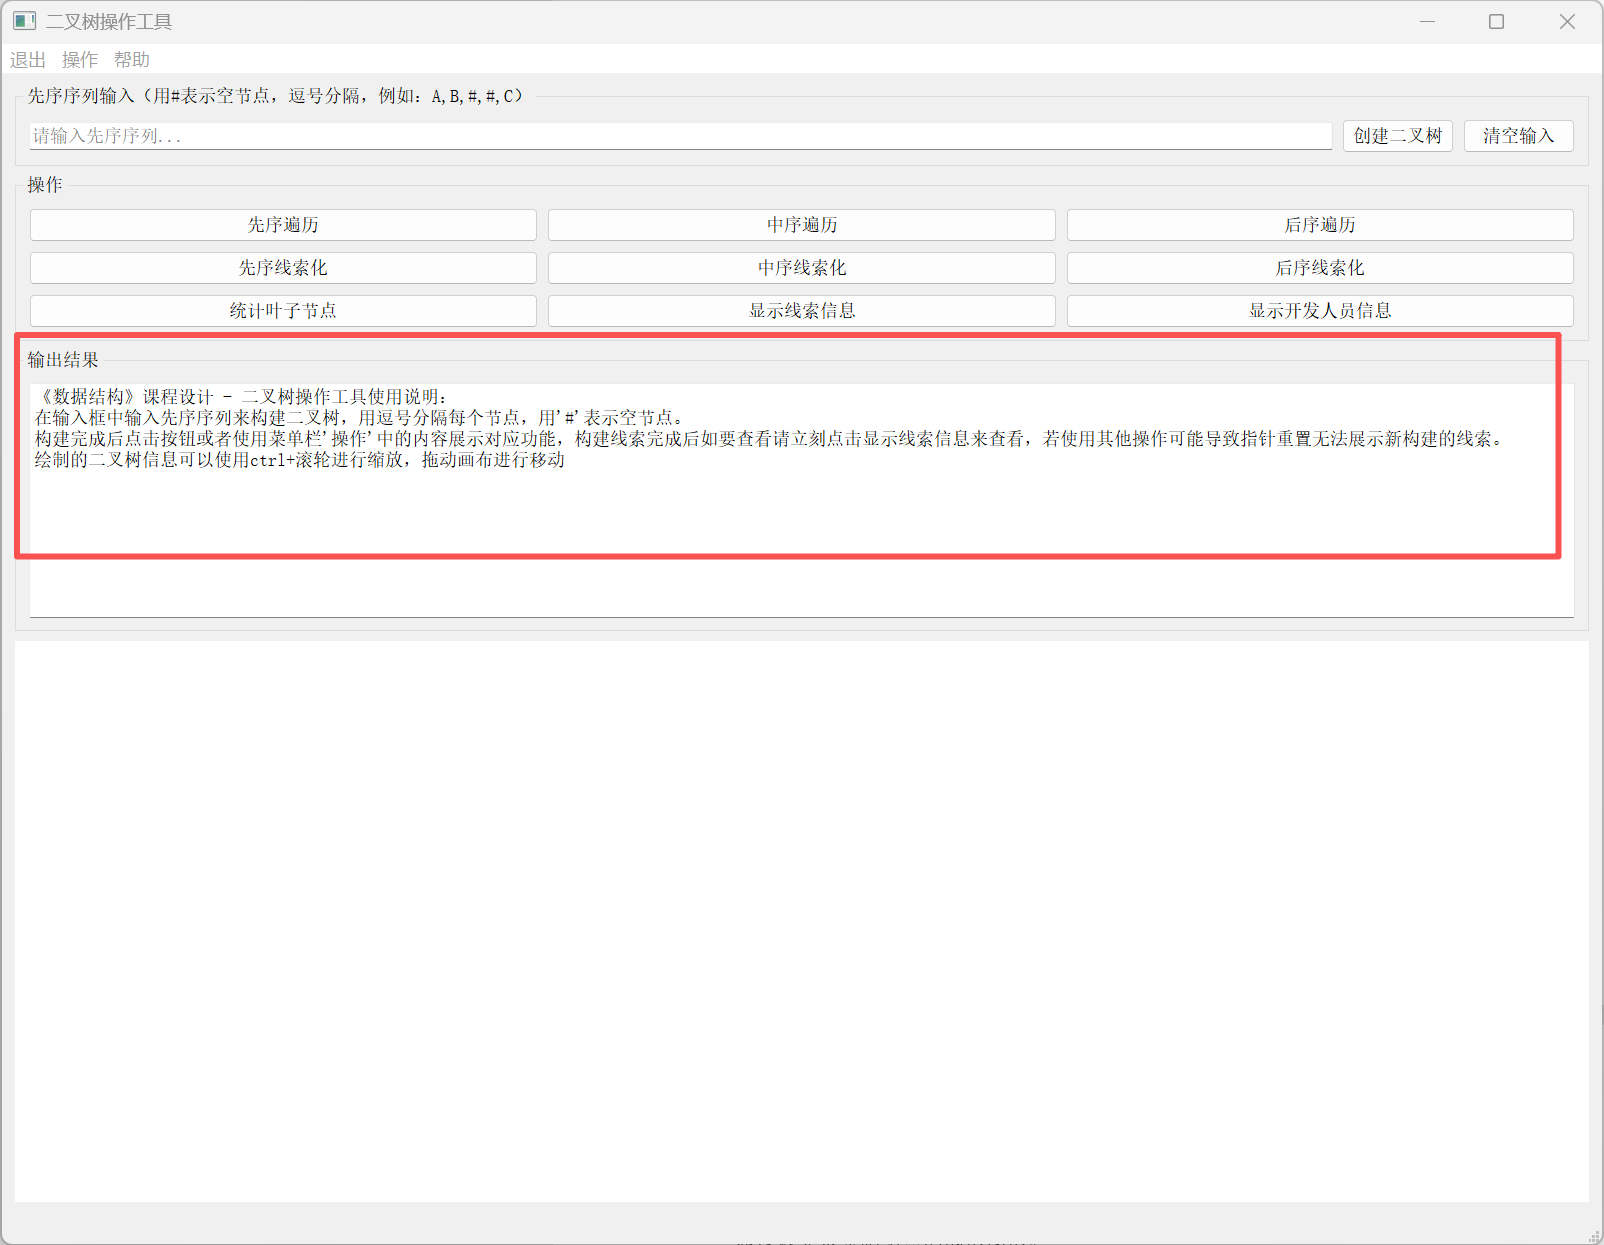
\includegraphics[width=0.5\textwidth]{pt1-3.png}
    \caption{菜单栏“帮助”实现效果}
\end{figure}
二叉树序列构建框是用户构建二叉树的地方,通过在构建框中按照指定格式输入想要用于构建二叉树的序列,然后再点击输入栏右侧的“创建二叉树”按钮即可实现二叉树的创建/修改。为了防止用户在输入一个较为长的二叉树序列之后难以清理,在右边还设置了一个清空输入的按钮,点击即可一键清除输入框中的内容。二叉树序列构建的提示在输入框的上方也有给出,需要注意的是,分隔符号“逗号”需要按照英文格式进行输入,否则会当做一个节点来处理。

在输入框下面即为操作按钮,这些按钮同样可以通过菜单栏进行使用。这里的操作包括实现题目要求的八大功能:先序/中序/后序遍历结果(结果会在下方的输出结果提示框中进行输出),先序/中序/后续线索化,叶子结点的统计以及线索化信息的展示。我还在最后增加了一个开发人员信息按钮,点击即可显示我的个人信息。

整个输出框在图形化界面中起到报错提示以及信息输出反馈的功能,类似于控制台的功能,用户可以根据输出框中的输出结果来判断操作是否发生错误并且修改操作。

最下方是画布功能,用户可以通过画布来观察自己创建的二叉树,这个画布还支持缩放、移动功能。
\subsubsection{二叉树的创建与叶子结点计算}
\noindent\textbf{功能说明:}

支持用户通过输入先序序列(以\#表示空节点、逗号分隔元素)创建二叉树,并实时统计树的总节点个数与叶子节点个数

\noindent\textbf{图形化界面说明:}

输入区域:界面顶部设有 “先序序列输入” 分组框,内置QLineEdit输入框,提示文本为 “请输入先序序列...”,用户需按格式(如A,B,\#,\#,C)输入序列;输入框右侧配有 “创建二叉树” 和 “清空输入” 两个按钮,分别用于触发树的创建和清空输入内容。

统计结果展示:点击 “统计叶子节点” 按钮后,结果会输出至下方 “输出结果” 文本框,格式为 “总节点个数:X 叶子节点个数:Y”,方便用户直观查看二叉树的节点构成。

可视化画布:界面下方的DrawWidget画布会在二叉树创建成功后,自动绘制树形结构,节点以蓝色圆形呈现,内部显示节点数据,父子节点间通过线段连接,支持缩放和平移操作以适配不同大小的树。

\noindent\textbf{实现方式说明:}

数据结构定义:

通过Node类定义二叉树节点,包含data(节点值)、left\_child/right\_child(左右孩子 / 线索指针)、left\_tag/right\_tag(标记,0 表示孩子,1 表示线索)等属性,为树的创建和后续操作提供数据载体。

树的创建逻辑:

在create\_binary\_tree函数中,采用递归方式处理用户输入的先序序列,遇到\#则返回空节点,否则创建新节点并递归构建左右子树,最终返回根节点。

节点统计算法:

count\_node函数:递归遍历树,若节点为空返回 0,否则返回 1(当前节点)加上左右子树的节点数,实现总节点统计。

count\_leaf\_node函数:递归遍历树,若节点为空返回 0,若节点无左右孩子则返回 1(叶子节点),否则返回左右子树的叶子节点数之和。

可视化绘制:

DrawWidget类继承QWidget,通过paintEvent实现树形绘制,先计算树的高度和宽度以动态调整节点半径和层间距,再通过draw\_tree递归绘制节点和父子连线,同时支持鼠标滚轮缩放和左键拖动平移。

\subsubsection{二叉树的遍历}

\noindent\textbf{功能说明:}

实现二叉树的先序、中序、后序三种递归遍历算法,遍历前自动重置节点线索标记(避免线索干扰),遍历结果实时输出至文本框,帮助用户验证遍历逻辑的正确性。

\noindent\textbf{图形化界面说明:}

操作按钮:在 “操作” 分组框第一行,设有 “先序遍历”“中序遍历”“后序遍历” 三个按钮,用户点击对应按钮即可触发相应遍历操作。

结果输出:遍历完成后,结果以 “[节点 1, 节点 2, ...]” 格式输出至 “输出结果” 文本框,例如先序遍历结果格式为 “先序遍历结果:[A, B, C]”。

状态提示:遍历过程中无额外弹窗,仅通过文本框输出结果,确保操作流程简洁;若未创建二叉树直接点击遍历按钮,文本框会提示 “请先创建二叉树!”。

\noindent\textbf{实现方式说明:}

遍历算法设计:

pre\_order\_traverse:递归访问当前节点,将节点值加入结果列表,再依次递归遍历左子树和右子树。

mid\_order\_traverse:递归遍历左子树,再访问当前节点并加入结果列表,最后递归遍历右子树。

pos\_order\_traverse:先递归遍历左子树和右子树,最后访问当前节点并加入结果列表。

线索重置机制:

遍历前调用reset\_thread\_tags函数,递归将所有节点的left\_tag/right\_tag重置为 0(孩子标记),并将线索指针置空,确保遍历仅基于真实的父子关系,避免线索干扰。

信号槽绑定:

在bind\_signals函数中,将三个遍历按钮的clicked信号分别与on\_pre\_order、on\_mid\_order、on\_post\_order槽函数关联,点击按钮时自动执行遍历逻辑并输出结果。

\subsubsection{二叉树的线索化}

\noindent\textbf{功能说明:}

实现二叉树的先序、中序、后序三种线索化算法,线索化后支持先序、中序线索树的遍历(后序线索树遍历暂未实现),同时提供线索信息查看功能,直观展示每个节点的线索指向。

\noindent\textbf{图形化界面说明:}

线索化操作按钮:在 “操作” 分组框第二行,设有 “先序线索化”“中序线索化”“后序线索化” 三个按钮,用户点击后触发对应线索化操作。

线索遍历结果:先序和中序线索化完成后,会自动执行线索树遍历并输出结果,格式为 “先序线索化完成,线索遍历结果:[节点 1, 节点 2, ...]”;后序线索化仅输出 “后序线索化完成”,不执行遍历。

线索信息查看:点击 “操作” 分组框第三行的 “显示线索信息” 按钮,文本框会以 “节点 X:左线索 / 孩子:Y,右线索 / 孩子:Z” 格式输出所有节点的线索状态,例如 “节点 A:左线索:None,右孩子:B”。

异常提示:若未创建二叉树直接点击线索化按钮,文本框提示 “请先创建二叉树!”;若未线索化直接点击 “显示线索信息”,提示 “请先创建二叉树并进行线索化!”。

\noindent\textbf{实现方式说明:}

线索化算法设计:

通过Thread类的静态方法实现三种线索化,核心是利用pre变量记录前驱节点,遍历过程中为空指针添加线索:

mid\_order\_threading:递归遍历左子树→处理当前节点线索(左空则指向pre,pre右空则指向当前节点)→更新pre→递归遍历右子树。

pre\_order\_threading:先处理当前节点线索→更新pre→若左孩子存在(left\_tag=0)则递归遍历左子树→若右孩子存在(right\_tag=0)则递归遍历右子树。

post\_order\_threading:递归遍历左子树→递归遍历右子树→处理当前节点线索→更新pre。

线索树遍历:

mid\_order\_thread\_traverse:从根节点出发,先找到最左节点,加入结果列表;再沿右线索遍历,最后进入右子树,循环直至节点为空。

pre\_order\_thread\_traverse:从根节点出发,先访问当前节点,若左孩子存在则进入左子树,否则沿右线索跳转,循环直至节点为空。

线索信息收集:

print\_thread\_info函数通过递归遍历树,收集每个节点的left\_tag/right\_tag状态及对应指针指向的节点值,整理为文本格式输出,帮助用户验证线索化结果。

\subsection{设计思想}

本次二叉树操作工具的开发,在结合数据结构理论知识与图形化开发的基础上,采用分层设计与模块化思想。我通过将系统拆解为数据处理、界面交互、逻辑调度三个核心模块,同时借鉴Model-View-Controller设计模式的分层理念,确保各模块负责内容独立、耦合度低。这样的方法使得代码的维护变得更加简单,再运行过程中如果出现错误只需要单独修改某一个特定部分,提升了代码的可维护性。
\subsubsection {分层设计思路}

\noindent\textbf {1.模型层}

模型层是整个工具的“逻辑核心”,仅负责二叉树的结构定义、核心算法实现,不涉及任何图形界面相关代码,确保算法可脱离界面独立运行与复用。

节点抽象:

通过Node类定义二叉树的基础数据单元,包含data(存储节点值)、left\_child/right\_child(双用途指针,既指向孩子节点也可作为线索指针)、left\_tag/right\_tag(标记位,0 表示指针指向孩子,1 表示指针指向线索),为后续树的创建、遍历、线索化提供统一的数据载体,避免因数据格式不统一导致的逻辑混乱。

算法封装:

将二叉树的关键操作(创建、遍历、线索化、节点统计)封装为独立函数,仅依赖Node类提供的接口实现逻辑,不与界面元素直接交互。例如,create\_binary\_tree函数通过递归处理先序序列构建二叉树,仅关注 “如何根据输入序列建立节点间的父子关系”,无需关心用户如何在界面输入序列;pre\_order\_threading等线索化函数,通过pre变量记录前驱节点,只关注“如何将空指针替换为线索”,不涉及线索的可视化展示,确保算法逻辑的独立性。

数据一致性保障:

考虑到线索化会改变节点指针的用途,在执行遍历操作前,我专门设计了reset\_thread\_tags函数,递归将所有节点的left\_tag/right\_tag重置为 0,并清空线索指针,避免线索干扰正常的遍历逻辑,确保每次遍历都基于二叉树的原始结构,保证结果准确。

\noindent\textbf {2.视图层}

视图层是工具与用户交互的“窗口”,仅负责接收用户输入、展示数据模型层的处理结果,不包含任何二叉树核心算法,通过预设的接口与其他模块协作,确保界面交互简洁直观。

界面组件划分:

按照功能相关性将界面拆分为输入、操作、结果展示三个核心模块,每个模块对应明确的用户操作场景:

输入模块:

以“先序序列输入”分组框为核心,包含QLineEdit输入框与“创建二叉树”,“清空输入”按钮,用户按格式(如 A,B,\#,\#,C)输入序列后,点击对应按钮即可触发树的创建或输入清空,输入框上方的提示文本可帮助用户理解输入规则,减少格式错误。

操作模块:

将功能按钮按用途分类排列(第一行遍历、第二行线索化、第三行用于其他功能),用户可快速找到目标操作;同时搭配菜单栏提供相同功能入口,满足不同用户的操作习惯,菜单栏中的“操作帮助”还能输出交互提示,降低第一次操作的用户的使用难度。

结果展示模块:

包含提示信息输出文本框与DrawWidget画布,文本框实时显示操作结果(如遍历序列、节点统计数据)与异常提示,画布则可视化展示二叉树结构,支持鼠标滚轮缩放与左键拖动平移,方便用户查看不同大小、不同复杂度的二叉树。

可视化逻辑独立:

DrawWidget类作为专门的绘图组件,仅负责二叉树的绘制工作,不干涉其他操作。它通过paintEvent事件实现树形绘制,先计算树的高度与宽度以动态调整节点半径和层间距(避免节点重叠并适配不同大小的树),再通过draw\_tree递归绘制节点与连线,仅需接收数据模型层传递的根节点,即可完成绘制。

\noindent\textbf {3.控制器层}

控制器层连接模型层与视图层,负责转发用户指令、同步数据与界面状态,避免模型与视图功能过分融合。

指令转发与结果回传:

基于Qt框架的“信号槽”机制,将视图层按钮的点击信号与控制器的槽函数(例如on\_pre\_order)绑定。当用户操作界面时,控制器接收视图层传递的输入数据,调用数据模型层的对应函数执行逻辑;模型层处理完成后,控制器再将结果传递给视图层,触发文本框更新或画布重绘。例如,用户点击“统计叶子节点”按钮时,控制器先调用count\_node与count\_leaf\_node获取总节点数与叶子节点数,再将结果格式化为文本框显示,实现“用户操作--逻辑处理--结果展示”的闭环。

状态同步与异常处理:

为避免用户因操作顺序错误或输入非法数据导致程序报错,控制器专门设计状态校验与异常提示逻辑。比如若用户未创建二叉树直接点击“遍历”或“线索化”按钮,控制器检测到数据模型层的根节点为空,不调用核心算法,直接向文本框输出“请先创建二叉树!”的提示;若用户输入空序列或格式错误的序列,控制器先校验输入合法性,再决定是否调用create\_binary\_tree函数,若校验失败则输出“输入序列格式错误,请按指定格式输入!”,引导用户修正操作。

\subsubsection {设计思路总结}
本次设计通过分层与模块化思想,使得完成的功能具有独立性,使得其具有较强的可复用性和可维护性。

在可复用性方面,数据模型层的核心算法不依赖界面,可直接复用至其他需要二叉树逻辑的项目中;视图层的DrawWidget画布组件,仅需接收根节点即可绘制二叉树,在开发过程中进行功能的扩充/修改时,无需修改画布代码,仅需在数据模型层新增对应创建函数。

在可维护性方面,各模块职责单一,修改某一功能时仅需调整对应模块代码,在代码实现过程中对逻辑进行调整时,仅修改了数据模型层的相关函数,无需改动视图层的按钮布局。

\subsection{逻辑结构与物理结构}

\subsubsection{逻辑结构}

由于本次课程设计的算法实现部分对应的是二叉树的遍历,因此逻辑结构对应的是处理与二叉树的建立、遍历、线索化等操作相关的类。这些操作基于树型结构这一种非线性数据结构。

\noindent\textbf {1.Node类}

作为二叉树所有节点的基类,Node类定义了节点的通用属性与接口,是逻辑结构的最小数据单元,能够反映节点之间的树形逻辑关系与线索逻辑关系。

Node类中属性如下:

data:存储节点值。

left\_child/right\_child:双用途指针,既可以表示左/右孩子节点,也可以用来指向线索节点。

left\_tag/right\_tag:标记,在0时表示是指向孩子节点的指针,1标志指向线索节点。

在构造时会将左右孩子指针设置为None,标签值默认为0。同时在类中也设置了相关函数用于返回当前Node的左/右孩子/线索等内容。

\begin{verbatim}
class Node:
    def __init__(self,data):
        self.data = data
        self.left_child = None
        self.right_child = None
        self.left_tag = 0
        self.right_tag = 0
\end{verbatim}

\noindent\textbf {2.二叉树操作函数}

这一部分内容围绕Node类封装了二叉树的创建,遍历,节点统计等算法,是逻辑结构实现的相关部分。

\begin{verbatim}
def create_binary_tree(pre_order):
    if not pre_order:
        return None
    data = pre_order.pop(0)
    if data == '#':
        return None
    node = Node(data)
    node.left_child = create_binary_tree(pre_order)
    node.right_child = create_binary_tree(pre_order)
    return node

def pre_order_traverse(node, result=None):
    if result is None:
        result = []
    if node:
        result.append(node.data)
        pre_order_traverse(node.left_child, result)
        pre_order_traverse(node.right_child, result)
    return result

def count_node(node):
    if not node:
        return 0
    if not node.left_child and not node.right_child:
        return 1
    return count_node(node.left_child) + count_node(node.right_child) + 1

def count_leaf_node(node):
    if not node:
        return 0
    if not node.left_child and not node.right_child:
        return 1
    return count_leaf_node(node.left_child) + count_leaf_node(node.right_child)
\end{verbatim}

这里仅展示了部分具有代表性的代码,比如二叉树的创建,先序遍历,叶子结点统计等。

\noindent\textbf {3.Thread类}

Thread类以静态方法封装先序、中序、后序线索化算法,核心是通过前驱节点记录,将节点空引用替换为线索,建立逻辑关系,优化遍历效率。

\begin{verbatim}
@staticmethod
    def mid_order_threading(root):
        pre = None
        def thread(node):
            nonlocal pre
            if not node:
                return
            thread(node.left_child)
            if not node.left_child:
                node.left_tag = 1
                node.left_child = pre
            if pre and not pre.right_child:
                pre.right_tag = 1
                pre.right_child = node
            pre = node
            thread(node.right_child)
        if root:
            thread(root)
            if pre and not pre.right_child:
                pre.right_tag = 1
                pre.right_child = None
\end{verbatim}

中序线索化代码如上所示。

在这一部分中我还构建了辅助逻辑函数reset\_thread\_tags用于递归重置节点线索标记与引用,恢复节点原始孩子关系,为遍历操作提供干净的逻辑环境。

\subsubsection{物理结构}

本次实验中,我采用了链式存储结构来存储二叉树数据,通过对象引用管连接点,使用Drawwidget类来进行图形化展示,确保数据信息和界面显示的同步。

采用链式存储的核心是将每一个节点作为独立内存对象,通过left\_child,right\_child引用来与其他节点建立关系。使用这种存储方式可以避免预设固定的内存空间,可以通过先序序列动态创建Node实例,对于任意复杂度的二叉树都可以适配。同事这种方式也对节点的添加,删除,线索化修改提供了更高的操作效率。

在构建一棵二叉树时,我们直接将根节点作为整个存储链表的起点,在后续操作时,入口均为这个根节点,以此向后来访问其他节点,实现数据的物理关联。

在进行可视化操作时,DrawWidget类直接接收根节点的Node实例,给予链式存储的引用关系来实现树形绘制,来确保物理存储与可视化展示的同步。

\subsection{开发平台}

计算机型号:华硕ROG枪神7

计算机内存:32GB

CPU:13th Gen Intel(R) Core(TM) i9-13980HX

操作系统:Windows11专业版

开发语言:python3.12

开发框架:PyQt5

开发环境:PyCharm 2025.2.0.1

运行环境:

PyQt5==5.15.11

PyQt5-Qt5==5.15.2

PyQt5\_sip==12.17.0

PySide6\_Addons==6.9.1

PySide6\_Essentials==6.9.1

setuptools==78.1.1

shiboken6==6.9.1

wheel==0.45.1

\subsection{运行说明}

运行方法:
\begin{verbatim}
    pip install 
    PyQt5==5.15.11
    PyQt5-Qt5==5.15.2
    PyQt5_sip==12.17.0
    PySide6_Addons==6.9.1
    PySide6_Essentials==6.9.1
    setuptools==78.1.1
    shiboken6==6.9.1
    wheel==0.45.1
    python UI.py
\end{verbatim}

或者在pycharm中运行UI.py即可

\subsection{系统的运行结果分析说明}
\subsubsection{二叉树的建立}
启动程序之后,用户可以通过在序列输入框中输入一个先序序列来构建一个二叉树,然后在空白画布上会绘制出依照这个先序序列构建的二叉树。

用户如果针对一个空序列构建二叉树,那么则会在输出框中给出提示报错。
\begin{figure}[H]
    \centering
    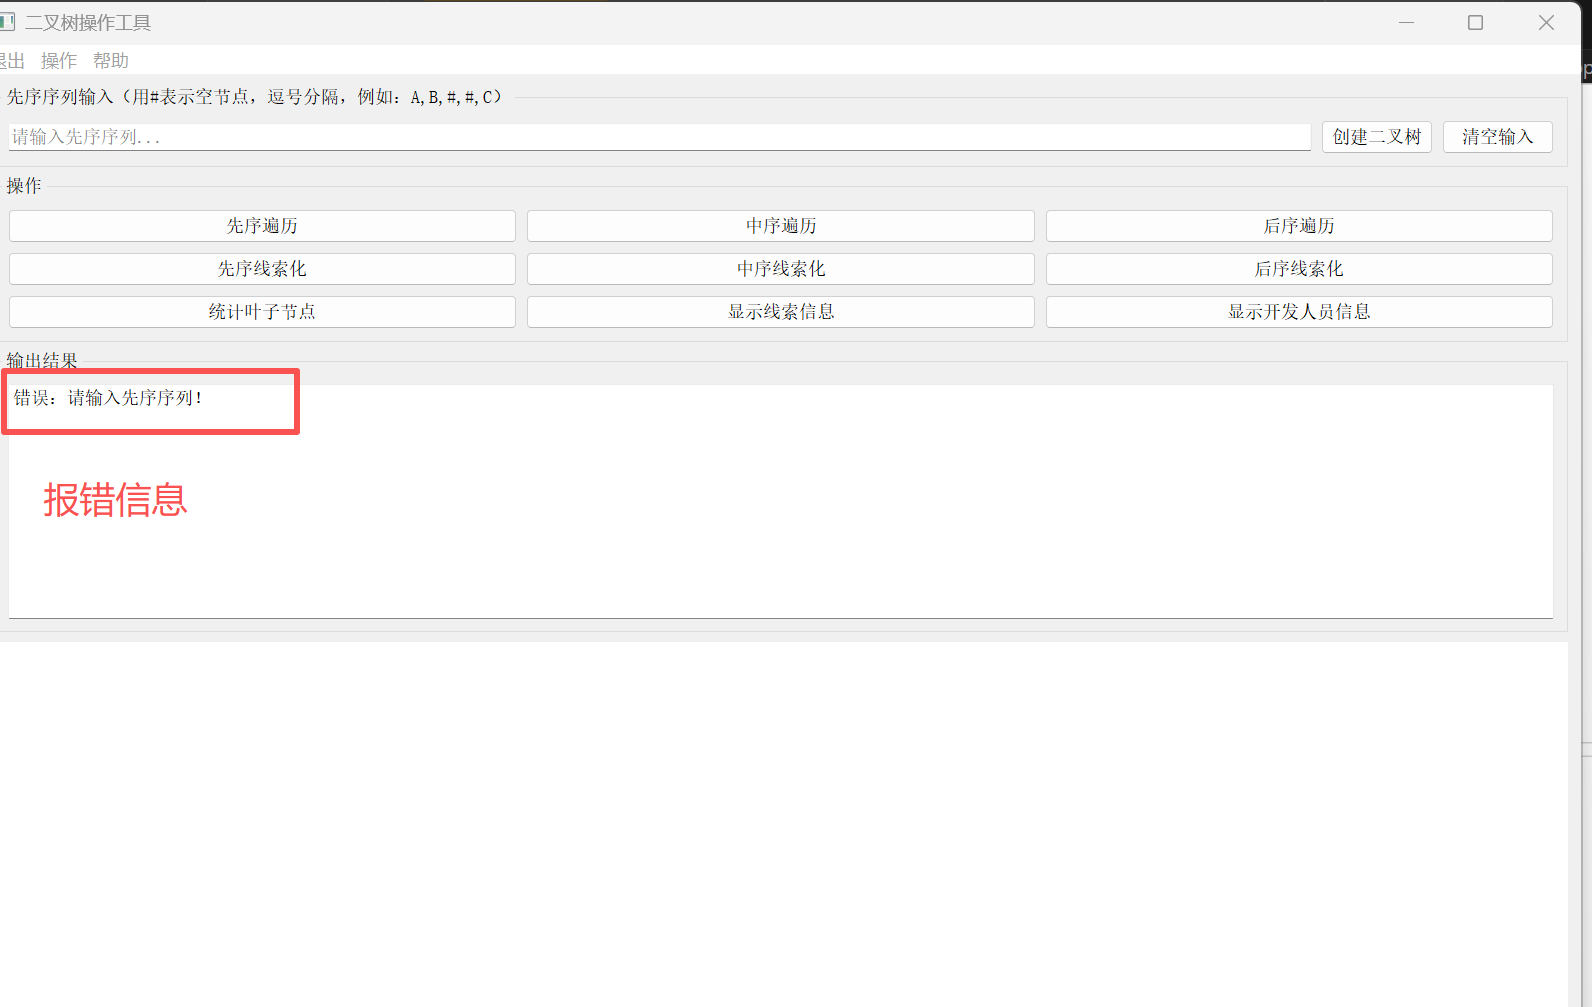
\includegraphics[width=0.5\textwidth]{pt1-4.png}
    \caption{对空序列构建二叉树报错}
\end{figure}

如果输入了一个正确的二叉树序列,那么就会提示二叉树成功创建,并且在画布上绘制出对应的二叉树。但是需要注意的是,由于二叉树的创建仅仅依赖先序序列,无法确定一个二叉树的形状,所以为了统一标准,在绘制时我统一先向左子树进行绘制,遇到“\#”判定为空节点之后,这个节点才不会继续往下生成。

同时我也考虑到了可能会存在错误序列输入的情况,比如“A,\#,\#,B”这样的序列,这样的序列肯定是不存在一个二叉树的,因为前面的某一部分已经能够构成一个完整的二叉树了,我们就会从前往后进行构建,直到出错的那个值之后进行截断,所以这样的序列的输出结果应当为A。

\begin{figure}[H]
    \centering
    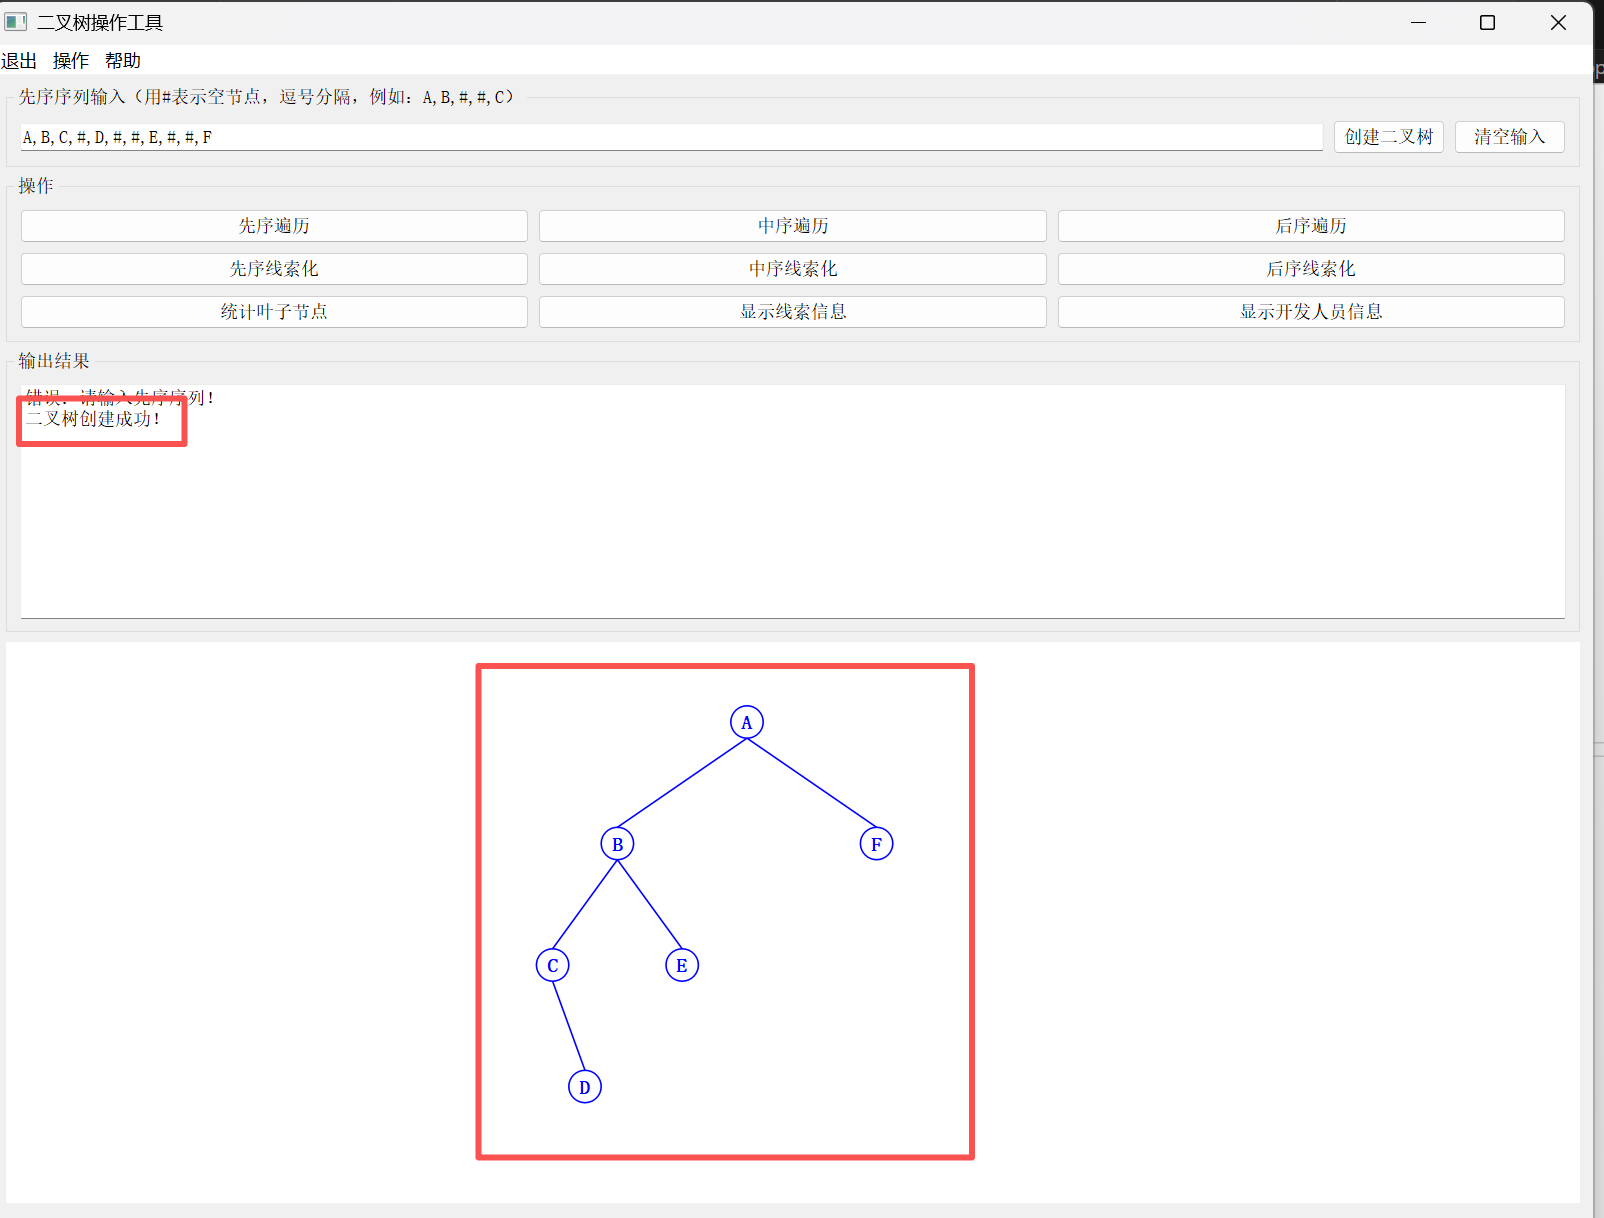
\includegraphics[width=0.5\textwidth]{pt1-5.png}
    \caption{二叉树的成功创建}
\end{figure}

\begin{figure}[H]
    \centering
    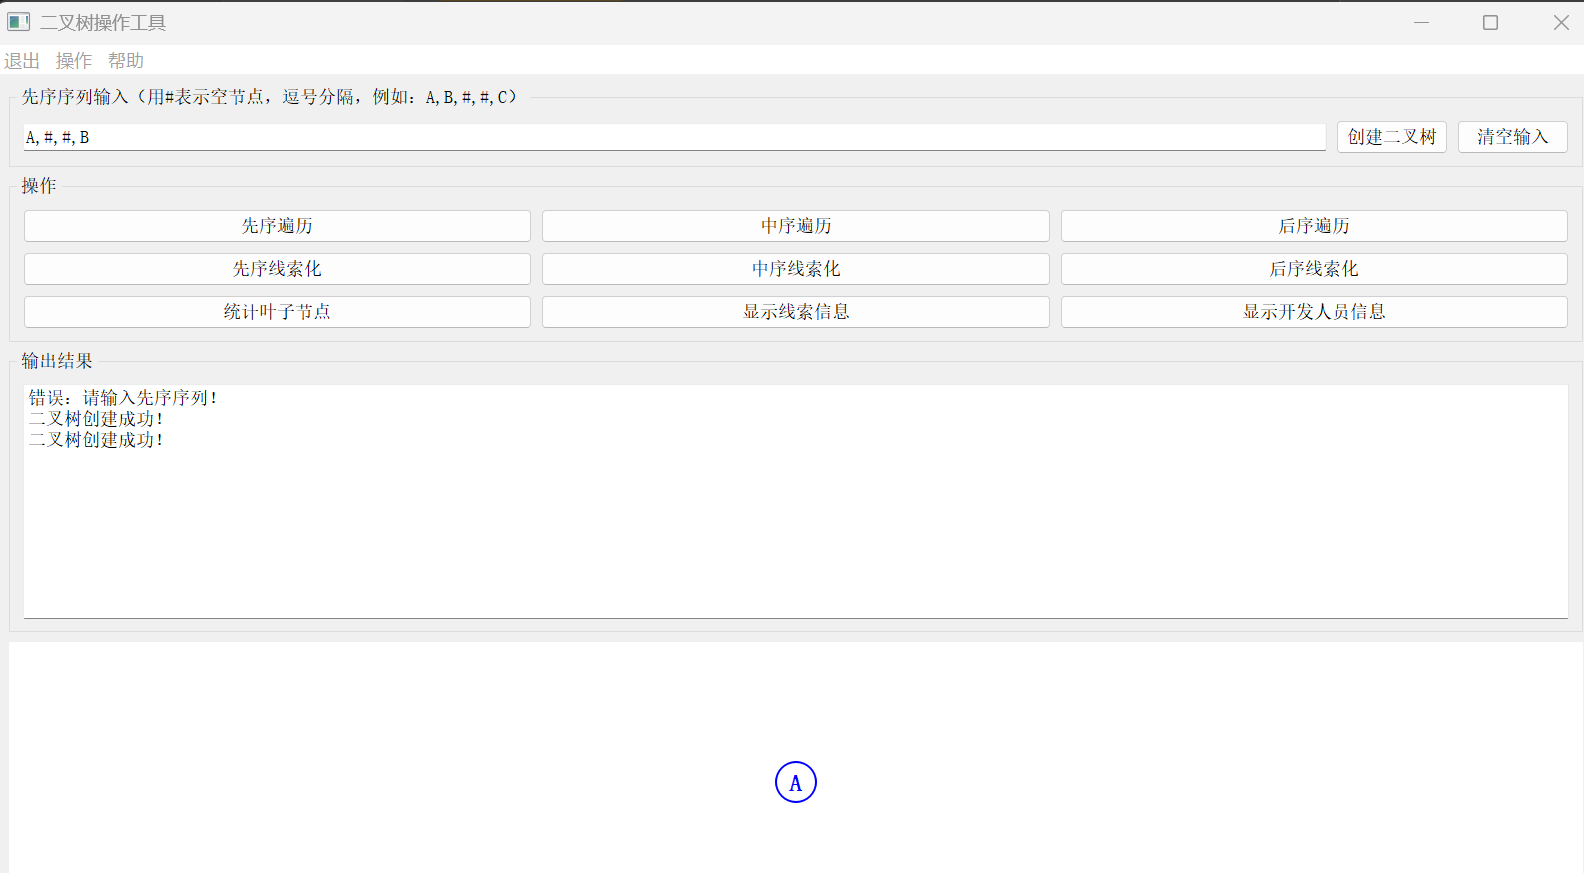
\includegraphics[width=0.5\textwidth]{pt1-6.png}
    \caption{错误序列的创建}
\end{figure}

\subsubsection{节点信息的统计}

点击操作按钮“统计叶子节点”就会在输出框中输出当前二叉树包含的总结点个数和叶子节点个数。

\begin{figure}[H]
    \centering
    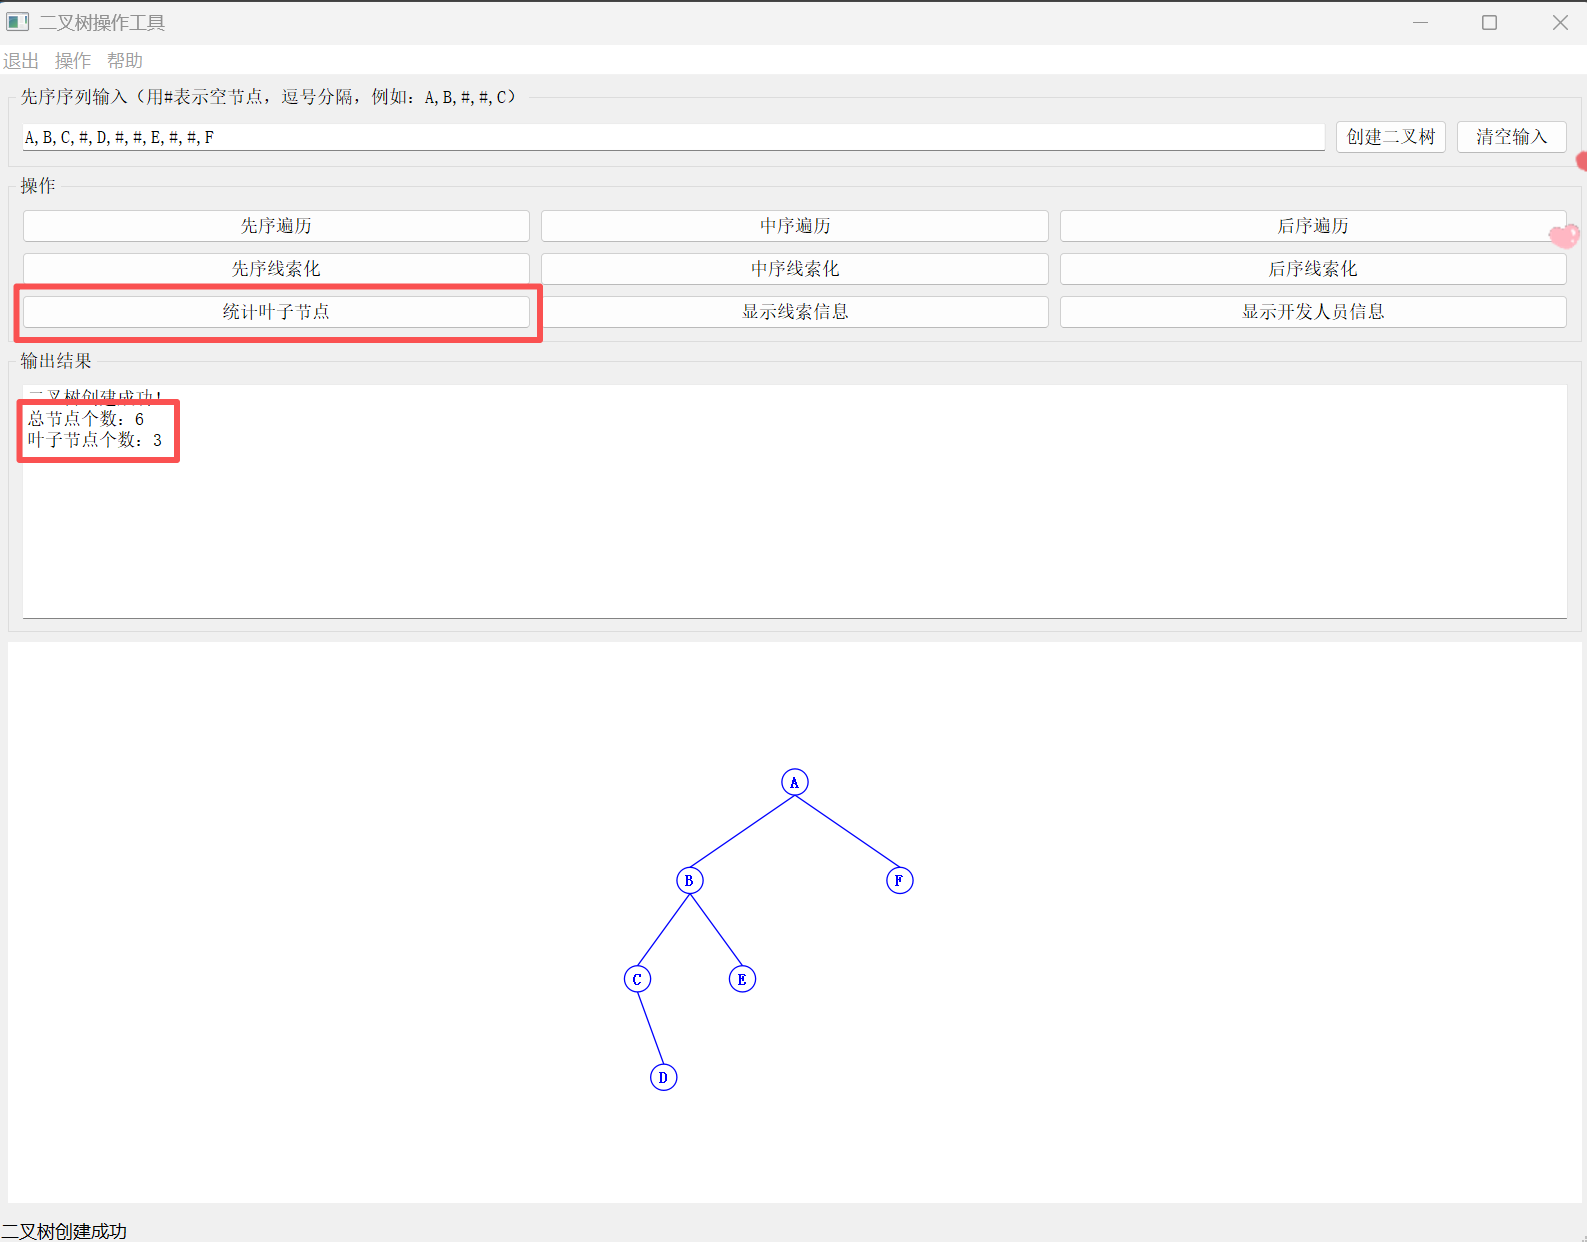
\includegraphics[width=0.5\textwidth]{pt1-7.png}
    \caption{节点统计}
\end{figure}

\subsubsection{二叉树的遍历}

在操作按钮中我设置了3个遍历按钮,点击相应的按钮即可在输出结果框中得到遍历顺序的结果。

\begin{figure}[H]
    \centering
    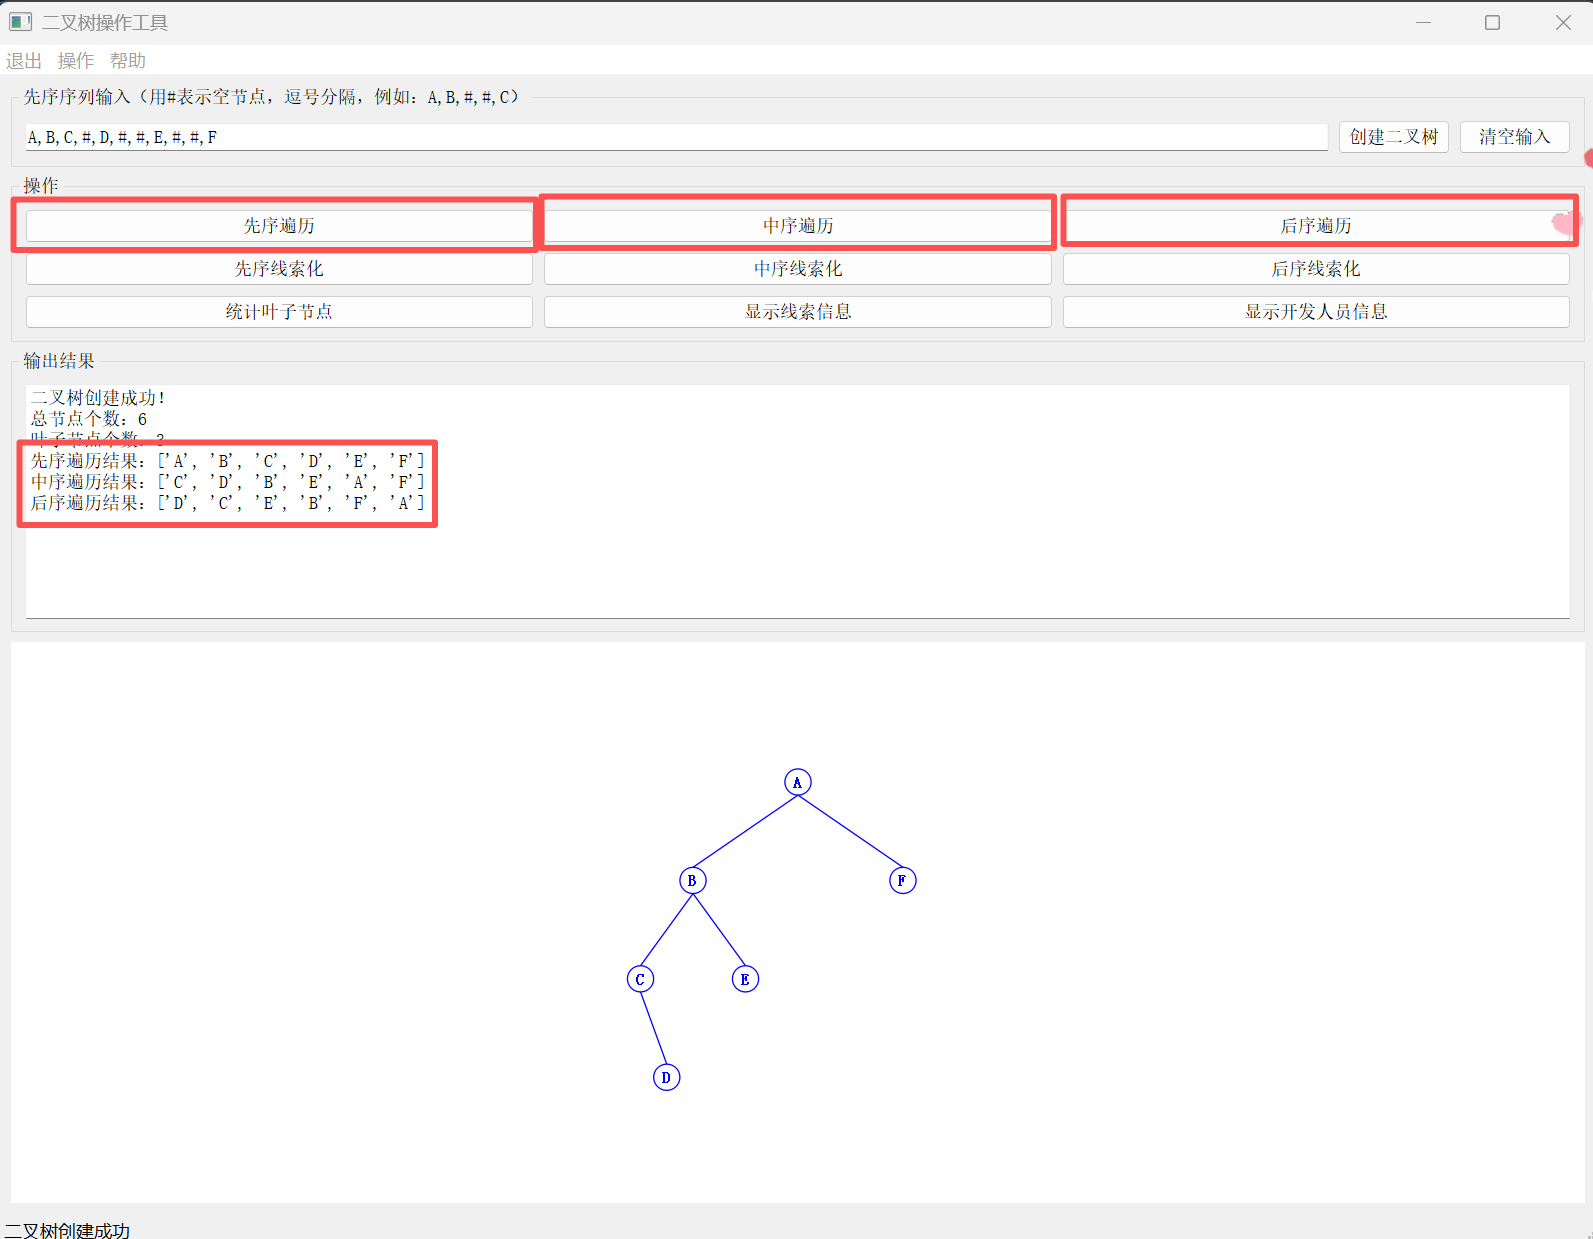
\includegraphics[width=0.5\textwidth]{pt1-8.png}
    \caption{二叉树遍历}
\end{figure}

\subsubsection{二叉树的线索化}

在第二行有三个按钮,可以实现二叉树的先序,中序和后序线索化,其中先序和中序线索化会输出对应的遍历结果。

\begin{figure}[H]
    \centering
    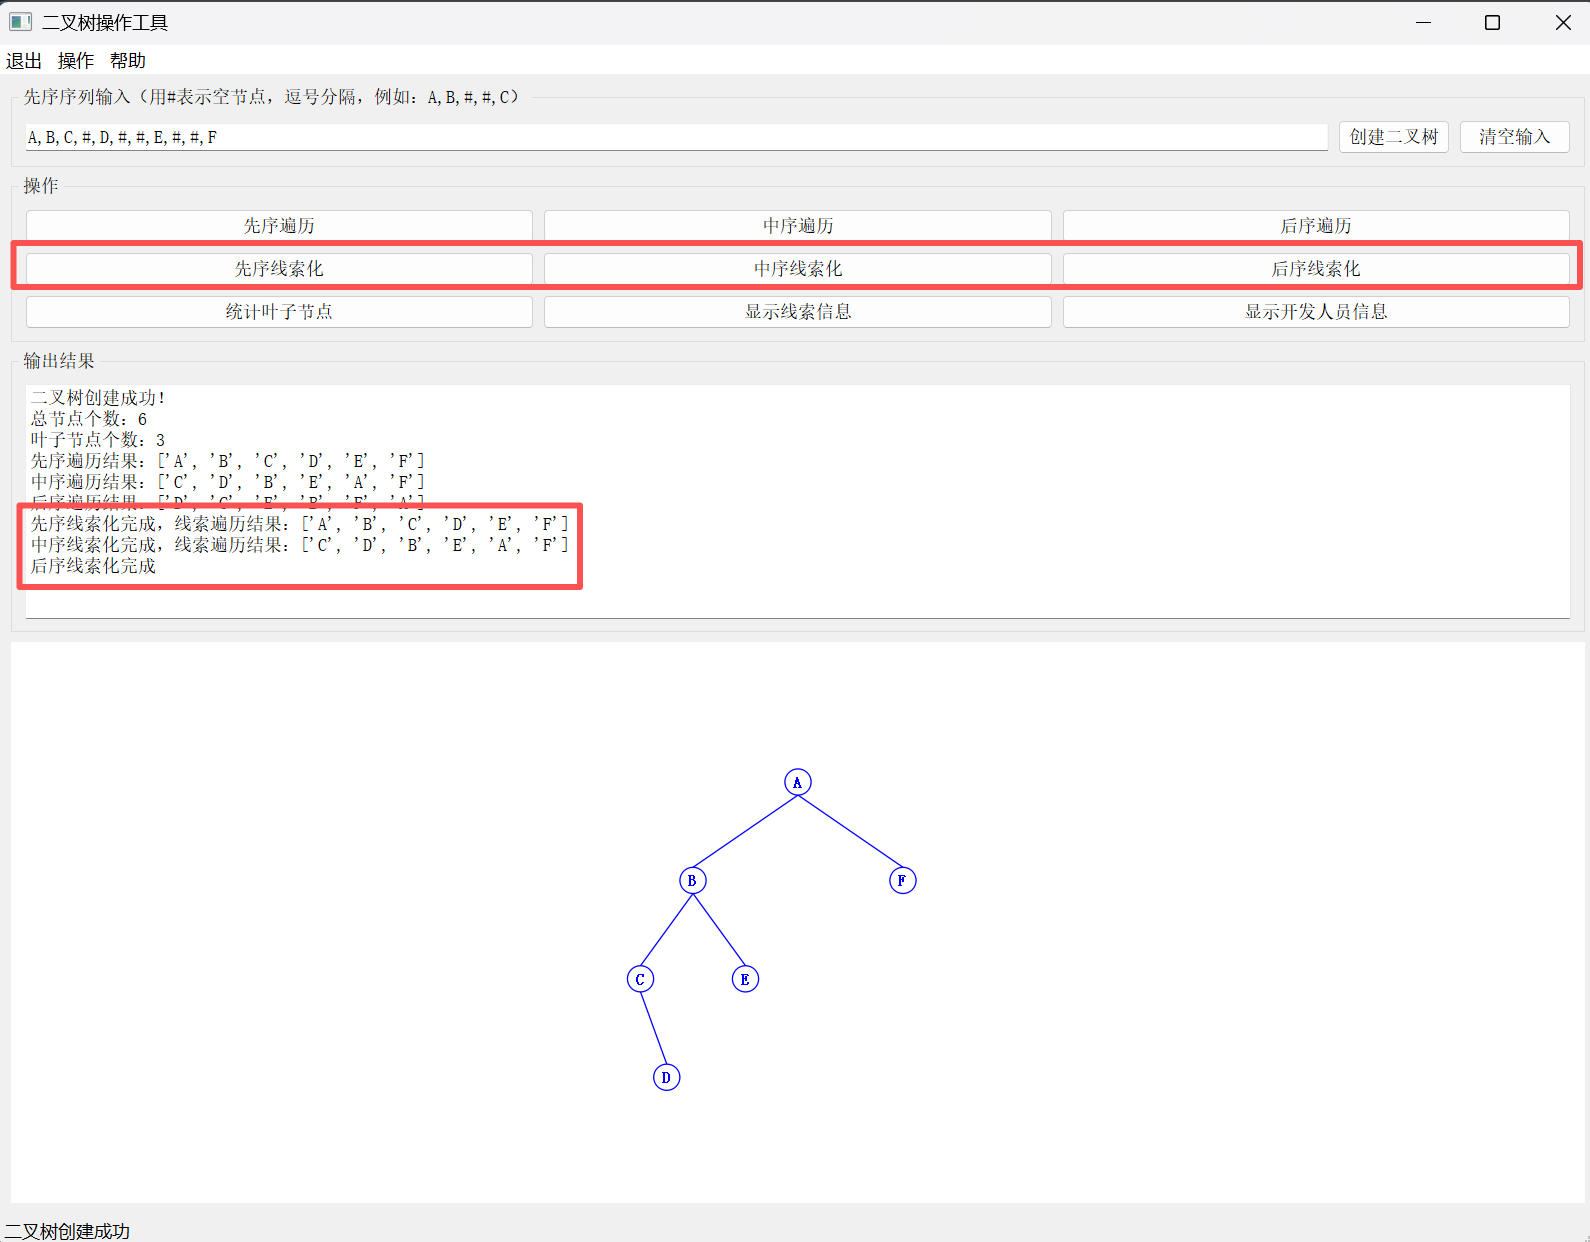
\includegraphics[width=0.5\textwidth]{pt1-9.png}
    \caption{二叉树线索化}
\end{figure}

如果想要看到每一次线索化之后的线索树的孩子指针,需要点击最后一行的“显示线索信息”按钮,就会输出当前线索化的信息。但是需要注意的是,由于在遍历等操作时,程序的执行为了防止孩子指向的错误会对指针进行重新初始化的操作,线索信息也会相应的出现改变,所以一定要及时点击该按钮以获取当前的线索信息。

\begin{figure}[H]
    \centering
    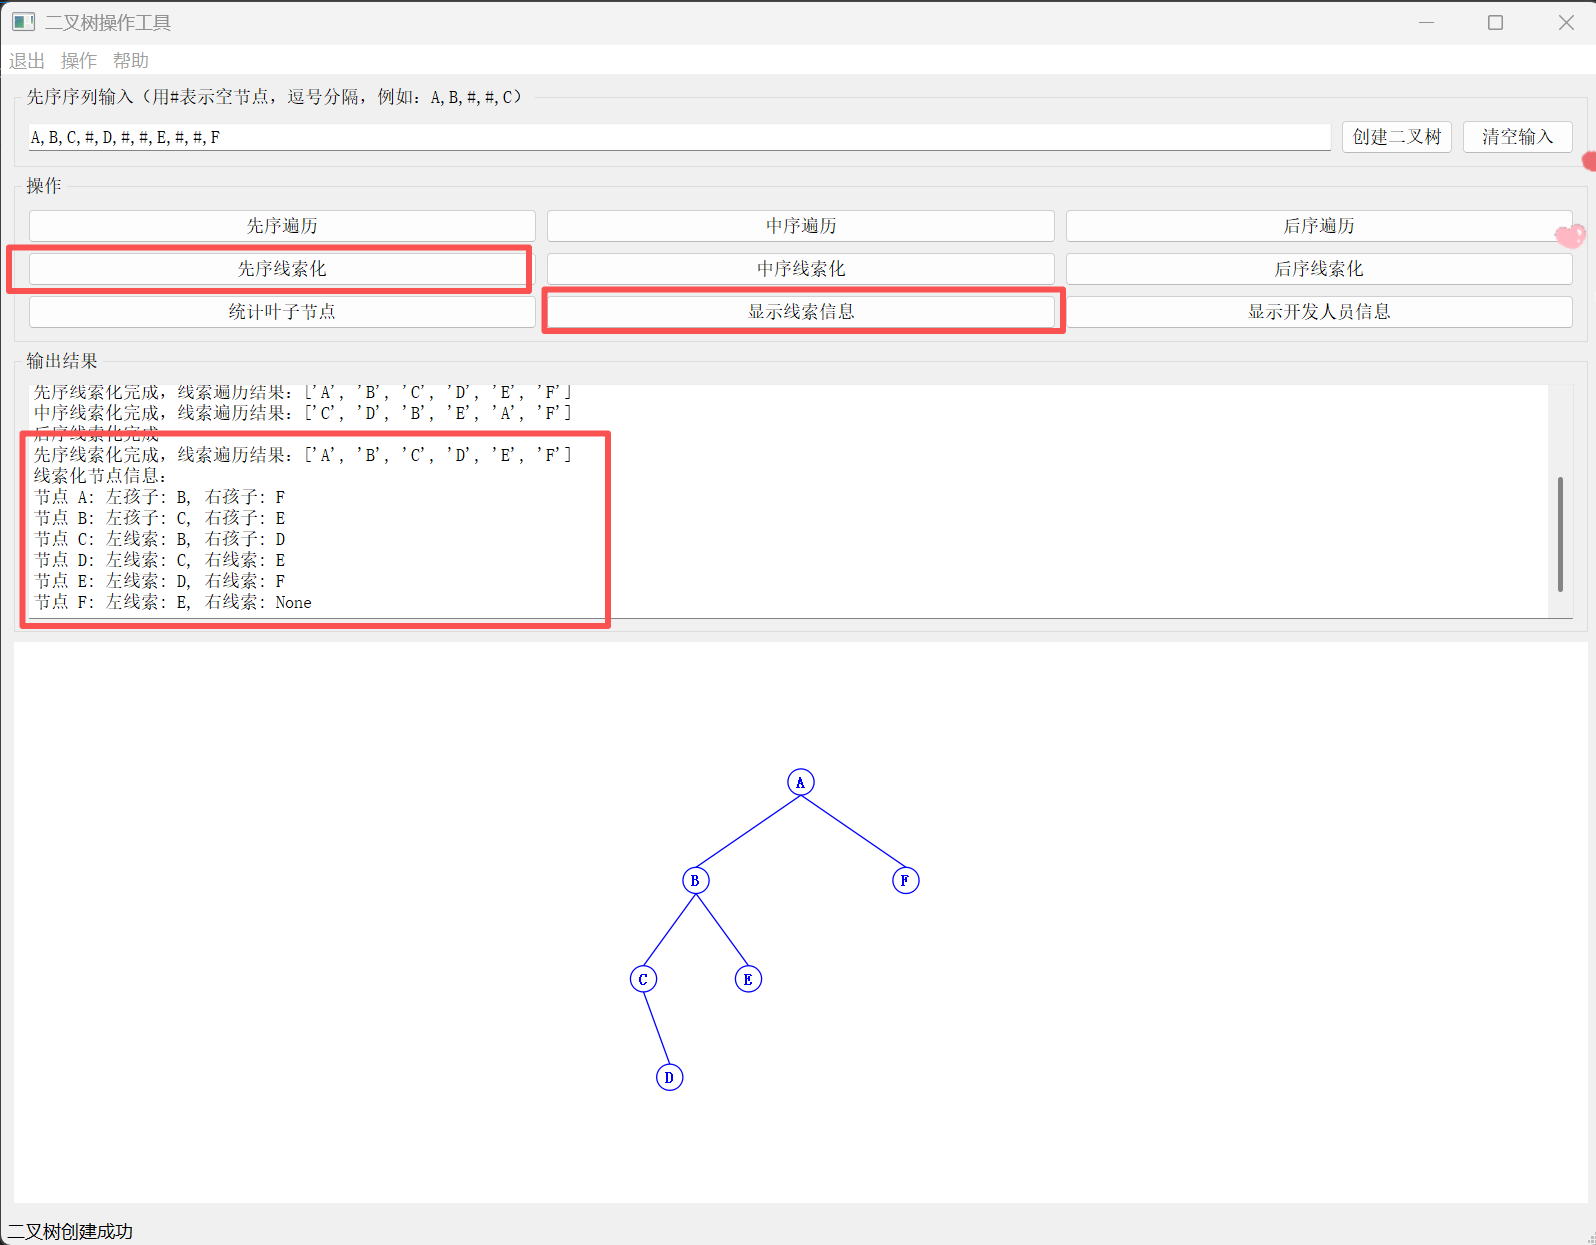
\includegraphics[width=0.45\textwidth]{pt1-10.png}
    \caption{先序线索化信息}
\end{figure}

\begin{figure}[H]
    \centering
    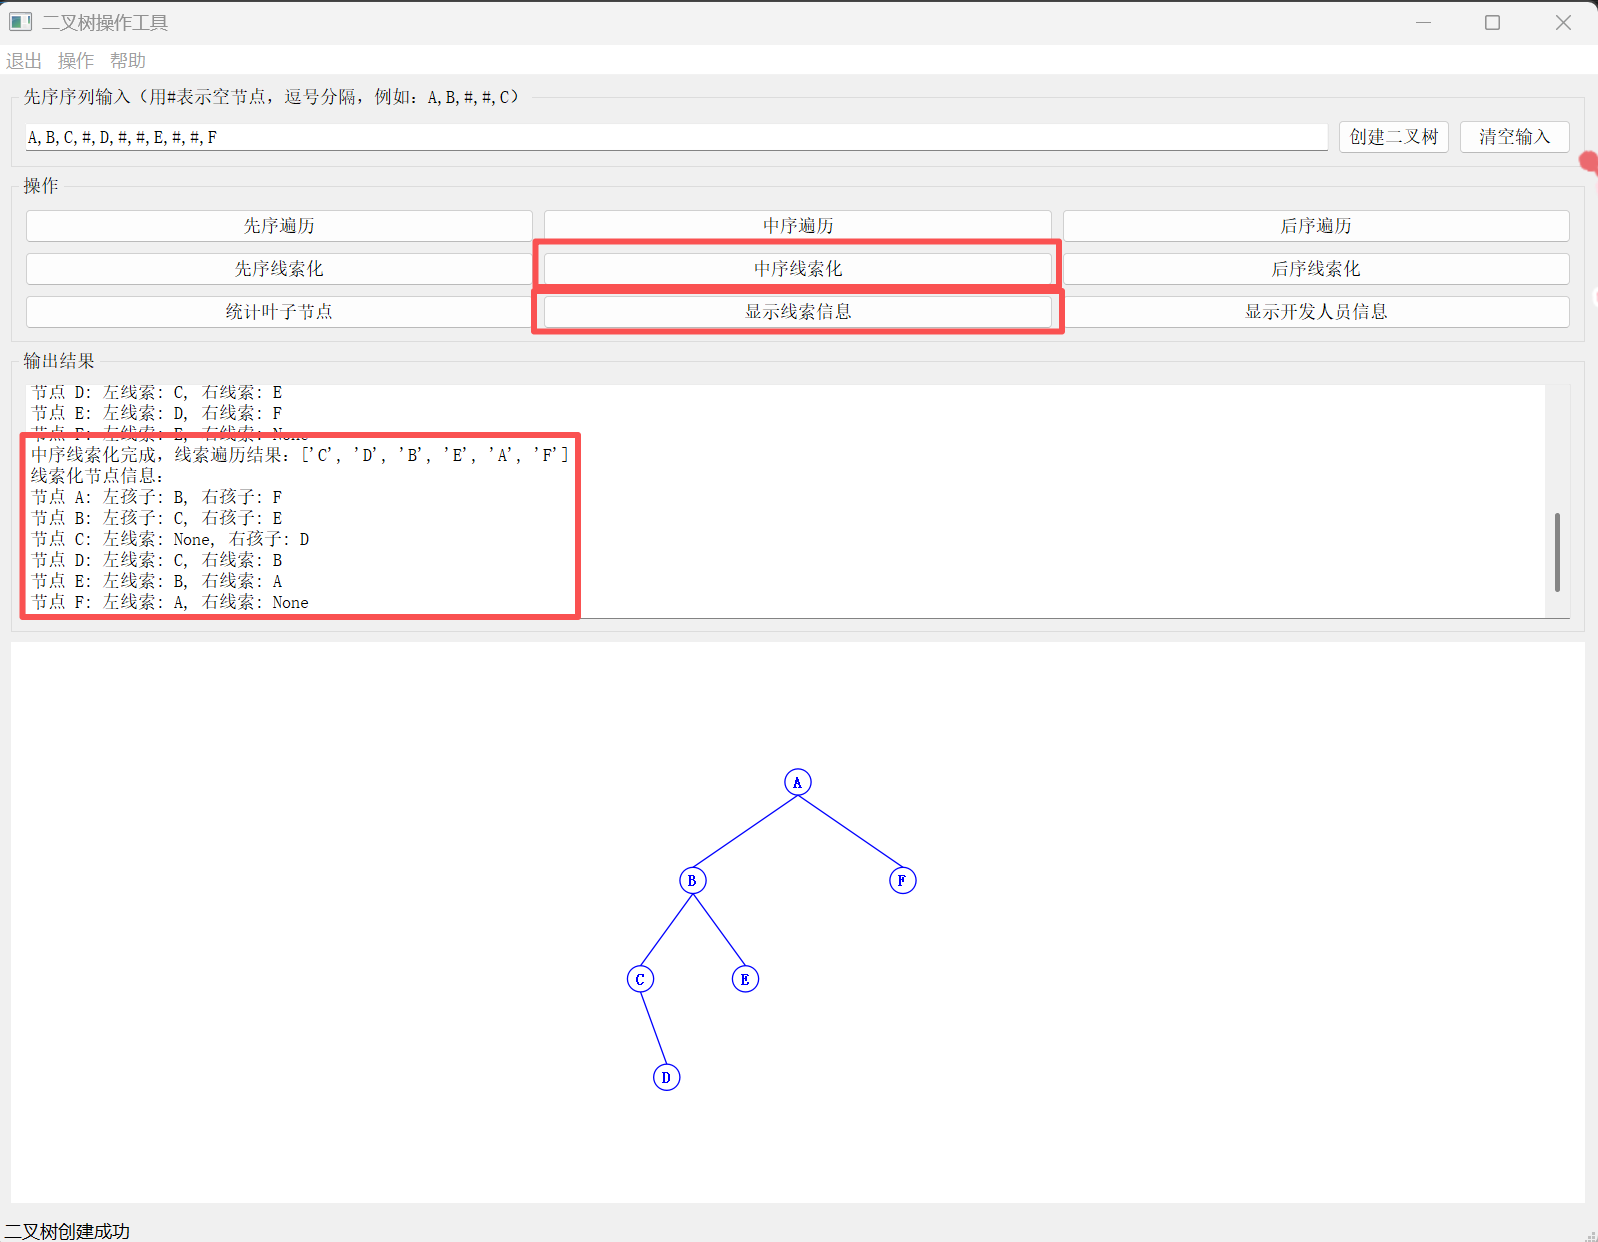
\includegraphics[width=0.45\textwidth]{pt1-11.png}
    \caption{中序线索化信息}
\end{figure}

\begin{figure}[H]
    \centering
    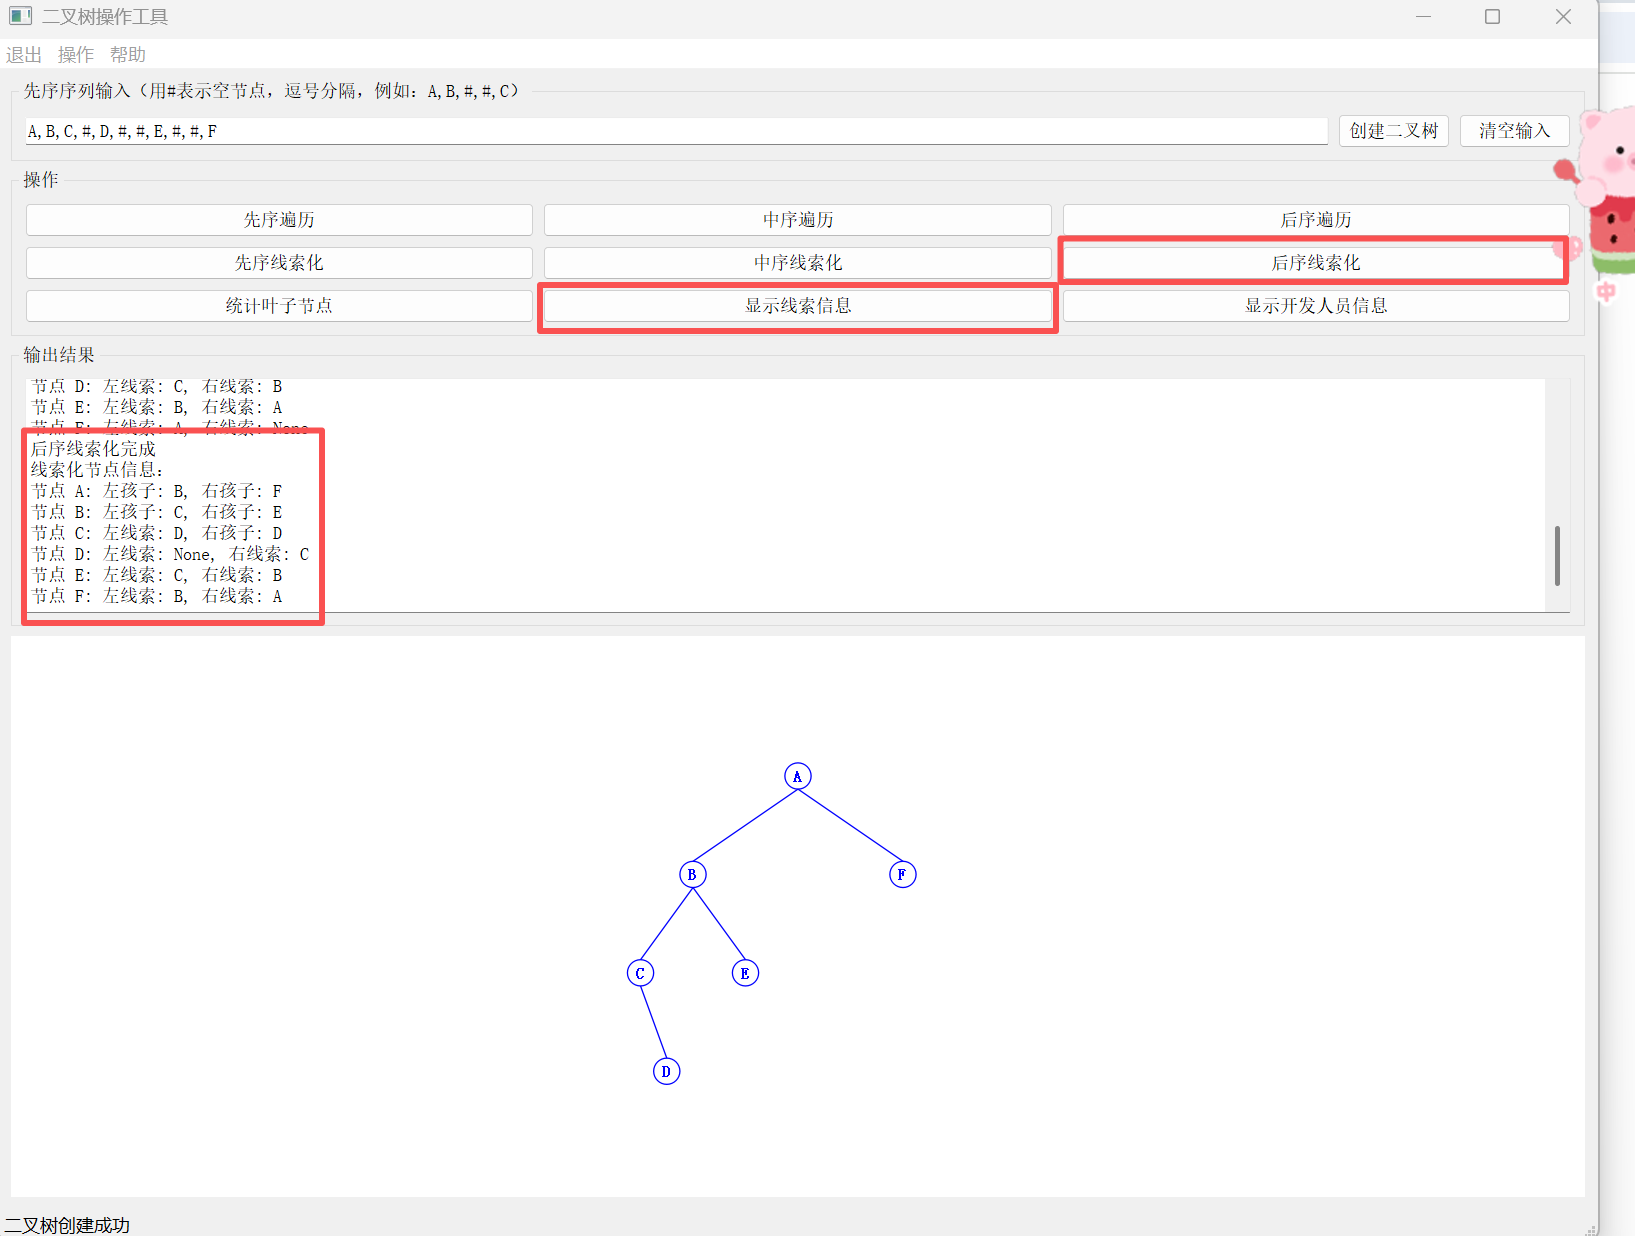
\includegraphics[width=0.45\textwidth]{pt1-12.png}
    \caption{后序线索化信息}
\end{figure}

如果此时进行一次先序遍历之后,再点击按钮显示线索信息,就会发现此时的线索信息已经变成了先序遍历时的初始化信息。

\begin{figure}[H]
    \centering
    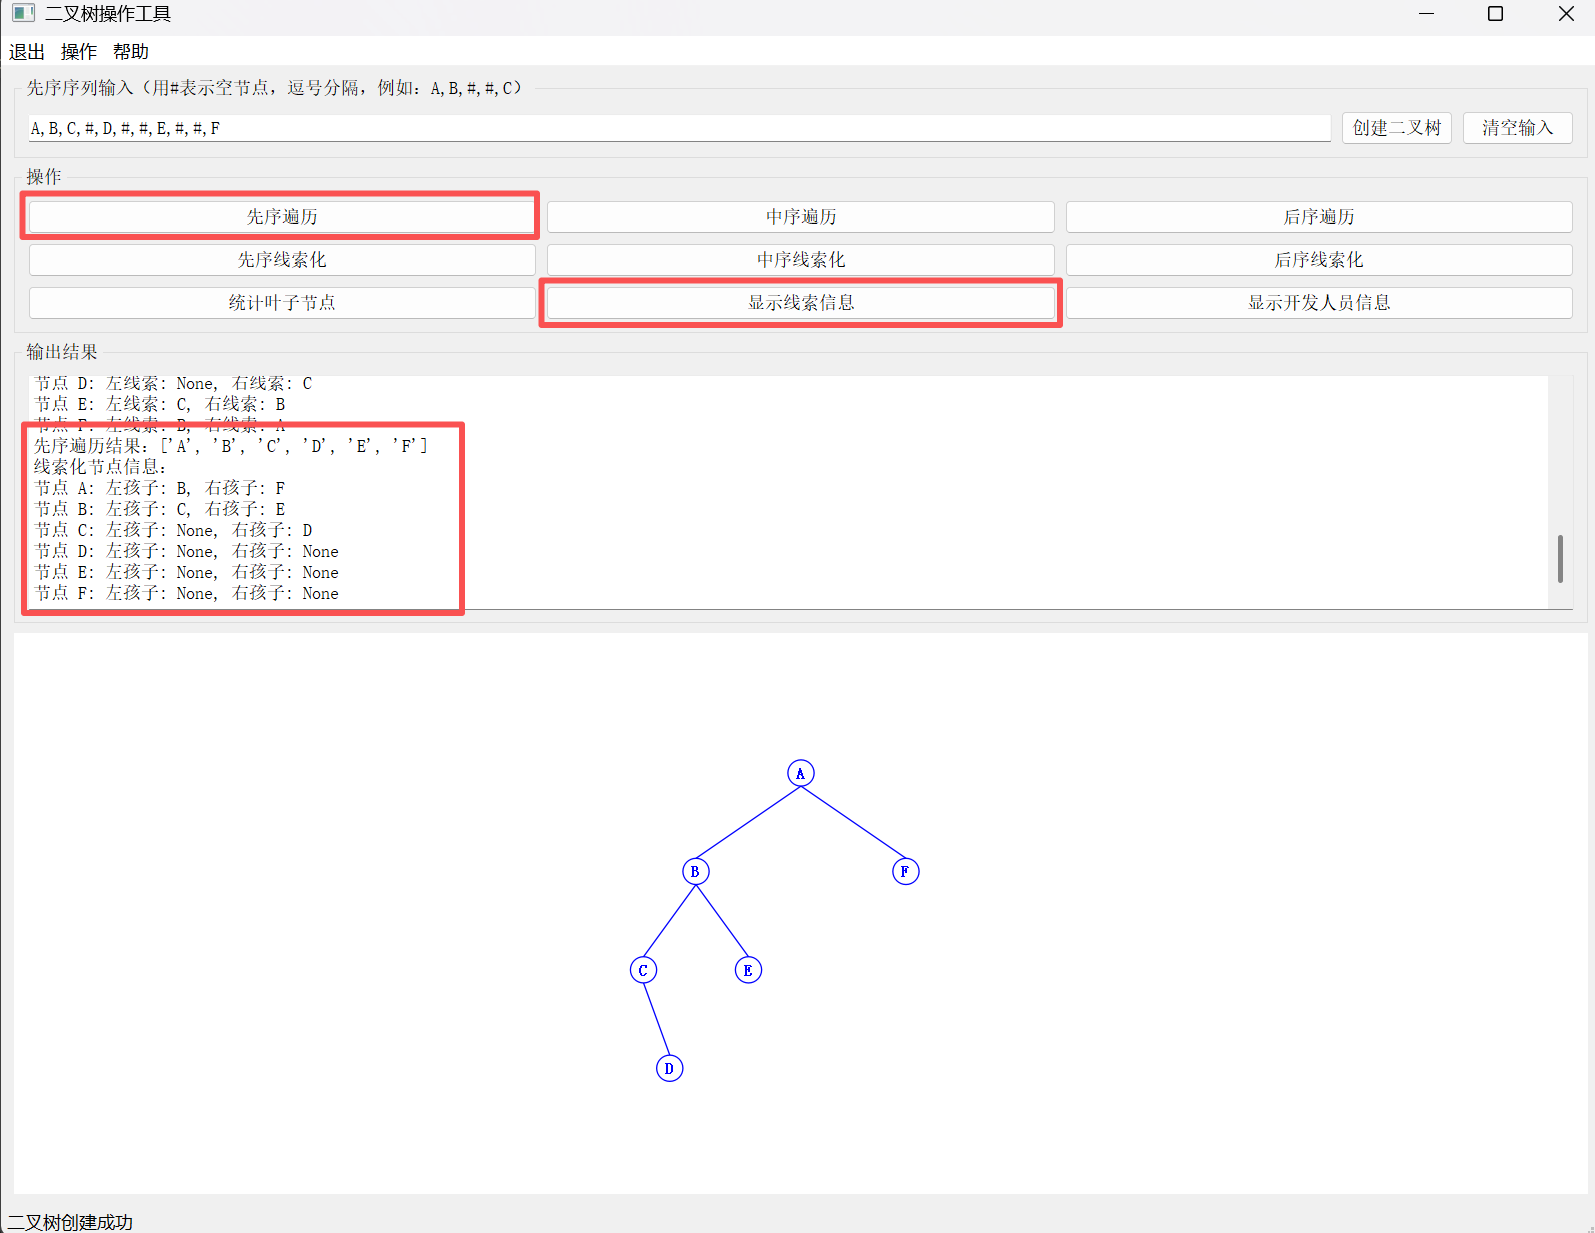
\includegraphics[width=0.5\textwidth]{pt1-13.png}
    \caption{遍历后初始化信息}
\end{figure}

\subsubsection{软件稳定性分析}

在软件开发过程中我也注意到了内存管理和对象的生命周期控制。但是在这一个项目中我并没有设计析构函数,而是通过python自带的GC机制和Qt框架的对象数模型来管理内存,通过控制引用关系来间接管理生命周期,从而避免内存泄漏。

Node实例的生命周期完全由GC机制进行管理,当构建一棵新的二叉树时,代码会调用create\_binary\_tree函数来生成全新的节点树,并且将根节点直接赋值给root。

\begin{verbatim}
self.root = create_binary_tree(pre_order.copy())
self.draw_widget.set_tree(self.root)
\end{verbatim}

root的赋值操作使得应用程序之前持有的旧二叉树根节点失去了唯一的强引用。只要DrawWidget中也同步更新了引用,旧的整棵二叉树结构就会成为不可达对象,等待并被GC自动回收。

对于UI对象来说,DrawWidget的生命周期由Qt的父对象树机制管理,当窗口被关闭时,Qt会自动递归地销毁所有子部件释放底层资源。

\newpage
\section{第二部分:综合应用设计}
\subsection{实现内容概述}
在某社会关系网络系统中,一个人属性包括所在地区、就读的各级学校、工作单
位等,每一人有众多好友,并可以根据个人兴趣及社会活动加入到某些群组。现需设计
一算法,从该社会关系网络中某一人出发,寻找其可能认识的人。例如根据两个人共同
好友的数量及所在群组情况,来发现可能认识的人;通过就读的学校情况发现可能认识
的同学。

1.通过图形化界面,显示某一人的社会关系网络。

2.寻找某一人可能认识的人(不是其好友),并查看这些人与其关联度(共同好友数)。

3.根据可能认识的关联度对这些人进行排序。

\subsection{软件功能}
\subsubsection{主界面}
用户可以在主界面加载用户并观察其关系网。
\begin{figure}[H]
    \centering
    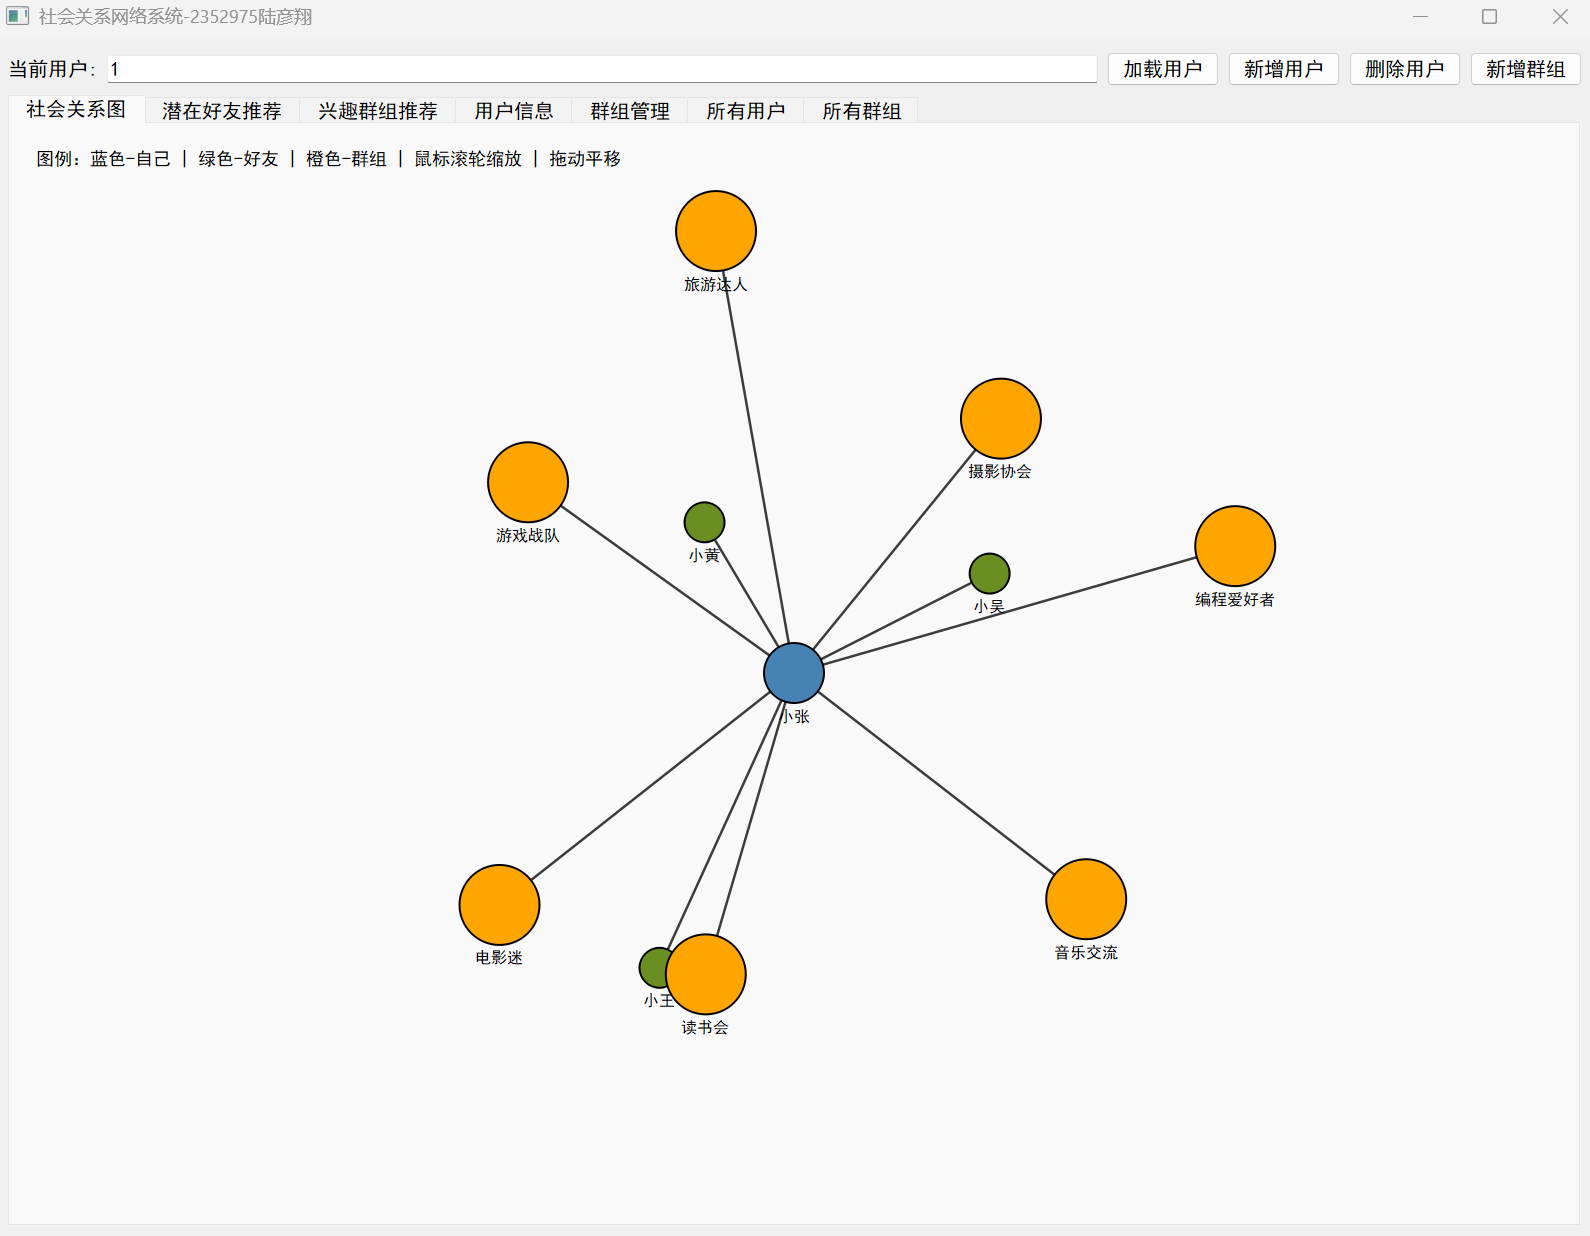
\includegraphics[width=0.5\textwidth]{pt2-1.png}
    \caption{主界面}
\end{figure}

在主界面最上端我设置了一个用户加载框,可以通过在其中输入不同的用户id然后点击加载按钮来更换不同的操作对象,可以显示不同用户的关系网并编辑其信息。同时还在输入框右边有删除用户,新增用户,新增群组这几个功能按钮。

在输入框下面设置了七个功能,第一个功能即为关系网的显示,还有潜在好友推荐,群组推荐,用户信息管理,群组管理,所有用户,所有群组这几个选项。

\subsubsection{社交关系可视化}

\noindent\textbf{功能描述:}

系统提供图形化界面展示用户的社交网络关系图,包括用户自身、好友和所属群组,支持节点的缩放、平移和高亮显示。不同颜色的节点用来区分不同类型,蓝色表示自己,绿色表示好友,橙色表示加入的群组,并且在节点上显示名称信息。在绘制节点时为了防止节点过分密集,我设置了三角和距离扰动,分别用于控制点的方位和距离,使得图像信息可以尽可能清晰,但是这也会导致每次生成的节点位置会有区别(内容不受影响)。

\begin{figure}[H]
    \centering
    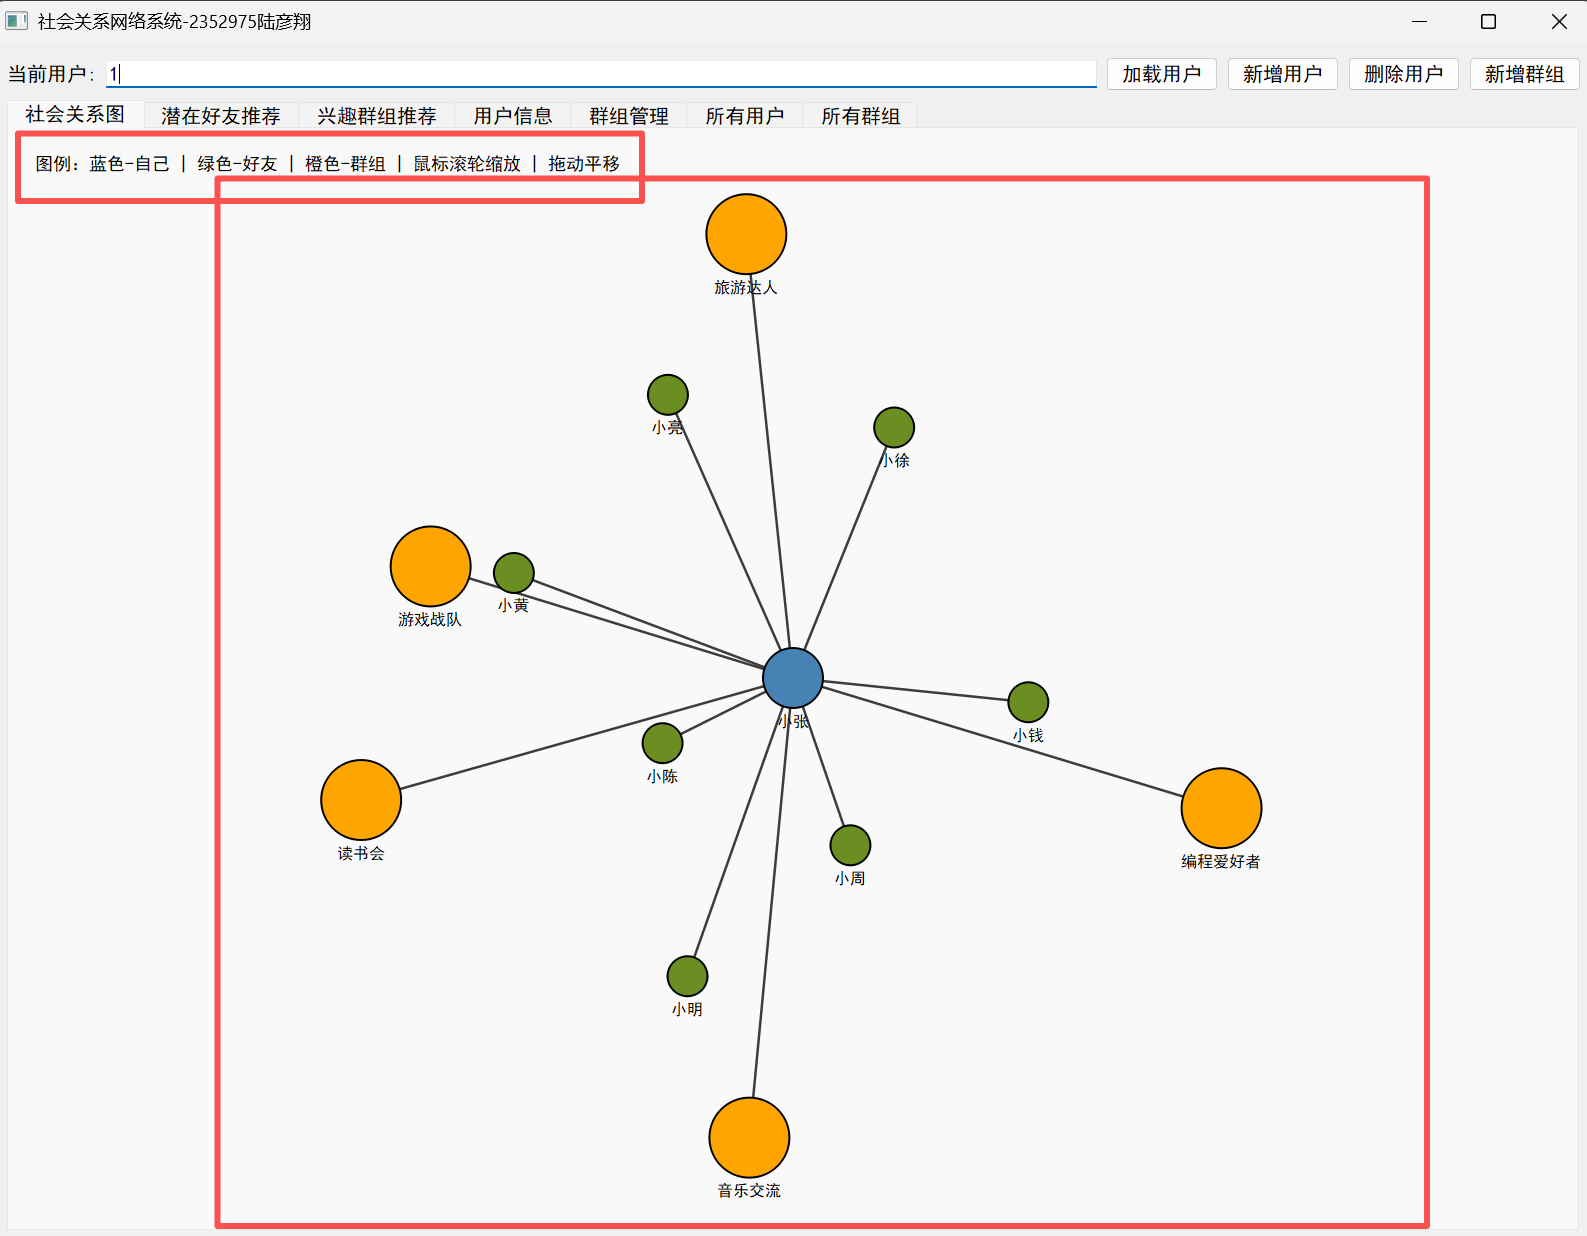
\includegraphics[width=0.5\textwidth]{pt2-2.png}
    \caption{关系可视化模块以及说明}
\end{figure}

\noindent\textbf{实现方式:}

在绘图实现方面,我是用了继承自Qwidget类的SocialGraphWidget,通过重写paintEvent方法来绘制节点和边。设置calculate\_node\_positions函数,通过极坐标随机扰动来避免绘制图像时不同节点之间重合。画板支持鼠标缩放和平移操作。

\subsubsection{好友推荐}

\noindent\textbf{功能描述:}

系统可以根据一个评价函数来从多个方面评判不同用户之间的关联,计算结果定义为相似度。在推荐好友时我设计了支持相似度排序和共同好友数量排序的方法,支持用户自选推荐数量并根据相关分数进行排序后推荐出top-k个潜在好友。系统会在列表中显示当前已经添加的好友和推荐的好友以及相关推荐依据(评分),用户可以通过添加好友/删除好友按钮来对个人好友列表进行修改,修改会实时反映在之前所说的关系图中。

\begin{figure}[H]
    \centering
    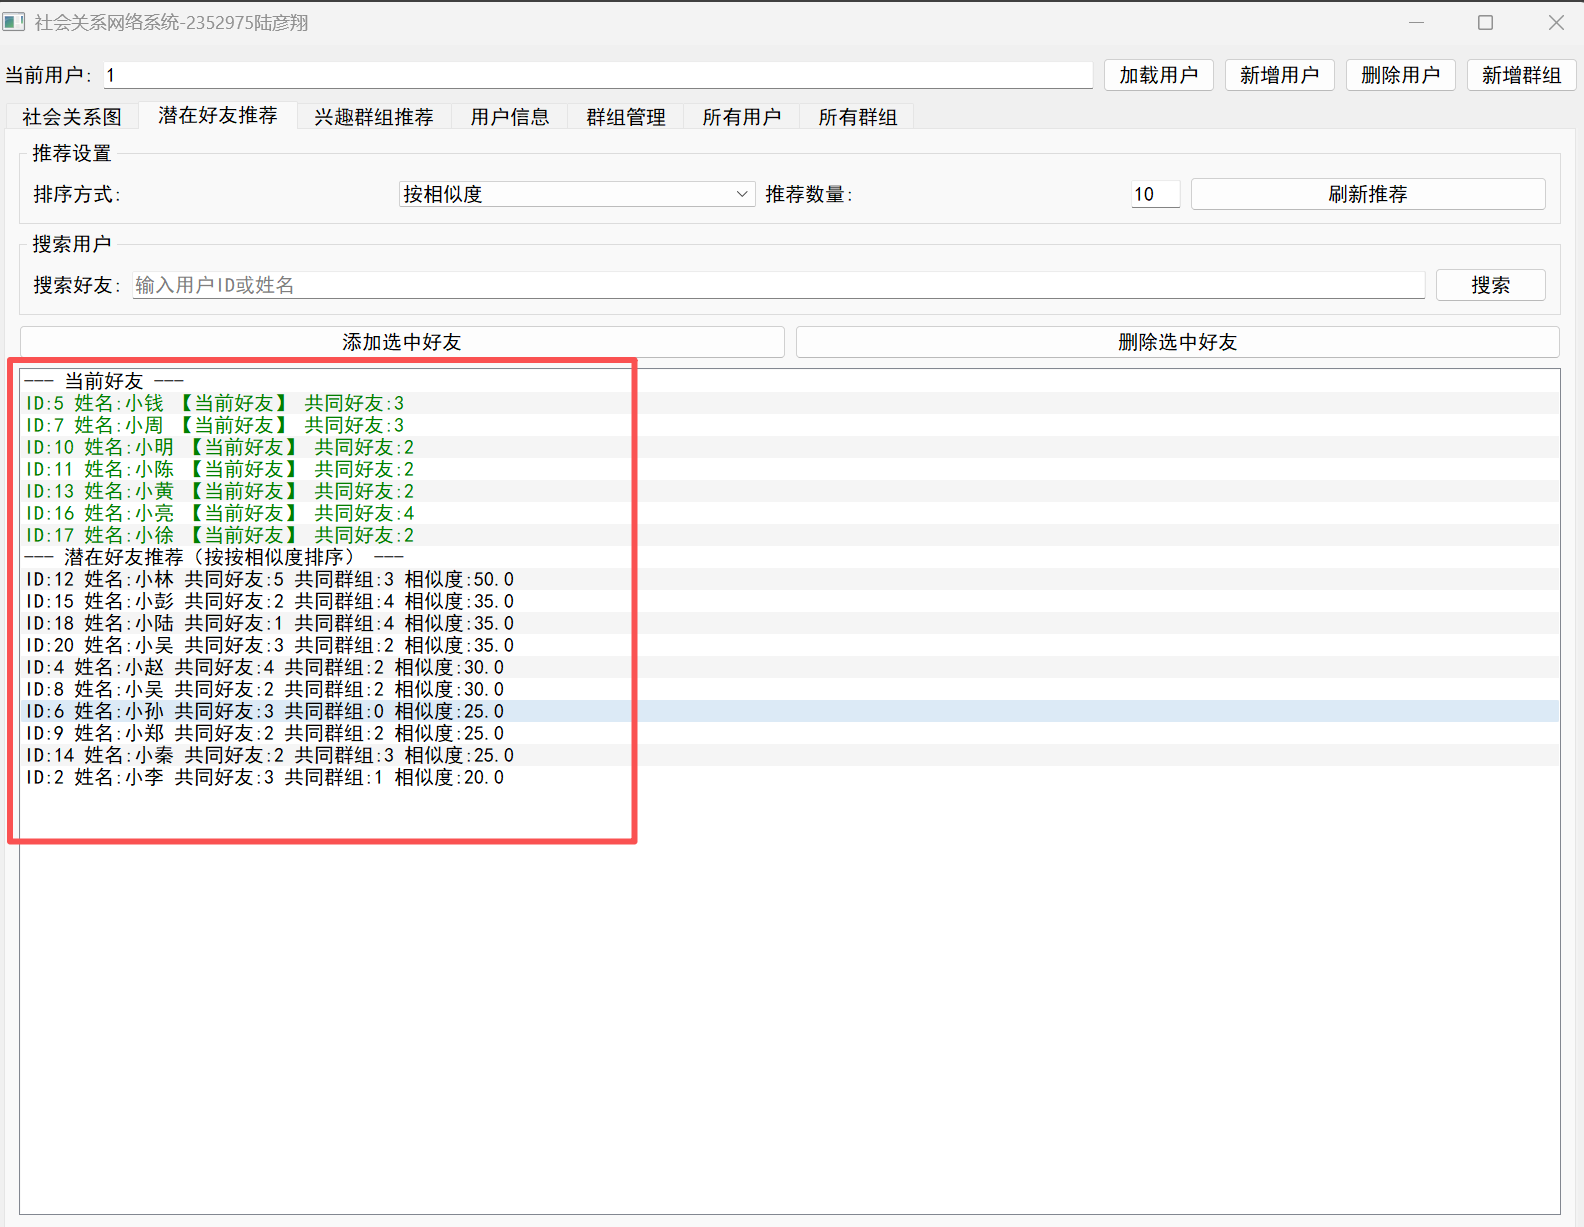
\includegraphics[width=0.5\textwidth]{pt2-3.png}
    \caption{在列表中显示已添加好友和推荐好友以及分数}
\end{figure}

\noindent\textbf{实现方式:}

这一部分的一个重要内容就是好友相似度的计算,为了考虑多个因素,我采用了加权求和的方式来进行相似度分数的计算。

\begin{verbatim}
        def calculate_similarity(self, user_id, candidate_id):
        user = self.network.get_user(user_id)
        candidate = self.network.get_user(candidate_id)
        if not user or not candidate:
            return 0
        similarity_score = 0
        common_friends = len(user.friends & candidate.friends)
        similarity_score += min(5 * common_friends,30)
        common_groups = len(user.groups & candidate.groups)
        similarity_score += min(5 * common_groups,20)
        common_schools = len(user.school & candidate.school)
        similarity_score += min(5 * common_schools,15)
        common_workplaces = len(user.workplace & candidate.workplace)
        similarity_score += min(7.5 * common_workplaces,15)
        if user.region == candidate.region and user.region != "":
            similarity_score += 5
        common_hobbies = len(user.hobbies & candidate.hobbies)
        similarity_score += min(5 * common_hobbies,15)
        return round(similarity_score, 2)
\end{verbatim}

在这里,我将共同好友的占比调整为30\%,共同学校占比调整为15\%,共同群组占比20\%,共同单位占比15\%,共同地区占比5\%,共同爱好占比15\%。这些占比在计算时设置相应的上限,每有一个共同项,在分数未达到上限时都会给出相应的加分。

考虑到题目要求中给出的根据共同好友数量进行排序,我在使用get\_potential\_friends方法生成推荐列表时支持了相似度排序和共同好友数量排序两种方案,可以通过页面中相关选择列表进行修改。

\subsubsection{兴趣群组推荐}

\noindent\textbf{功能描述:}

结合好友推荐的方法,我还为每个用户设计了群组推荐窗口,方便每个用户通过群组标签来找到自己可能感兴趣的群组。这一部分实现的核心点在于用户个人信息与群组标签的匹配。我同样为这一部分内容设置了一个匹配分数match\_point,通过计算当前用户和不同群组之间的匹配分数来获取top-k个群组推荐。

\begin{figure}[H]
    \centering
    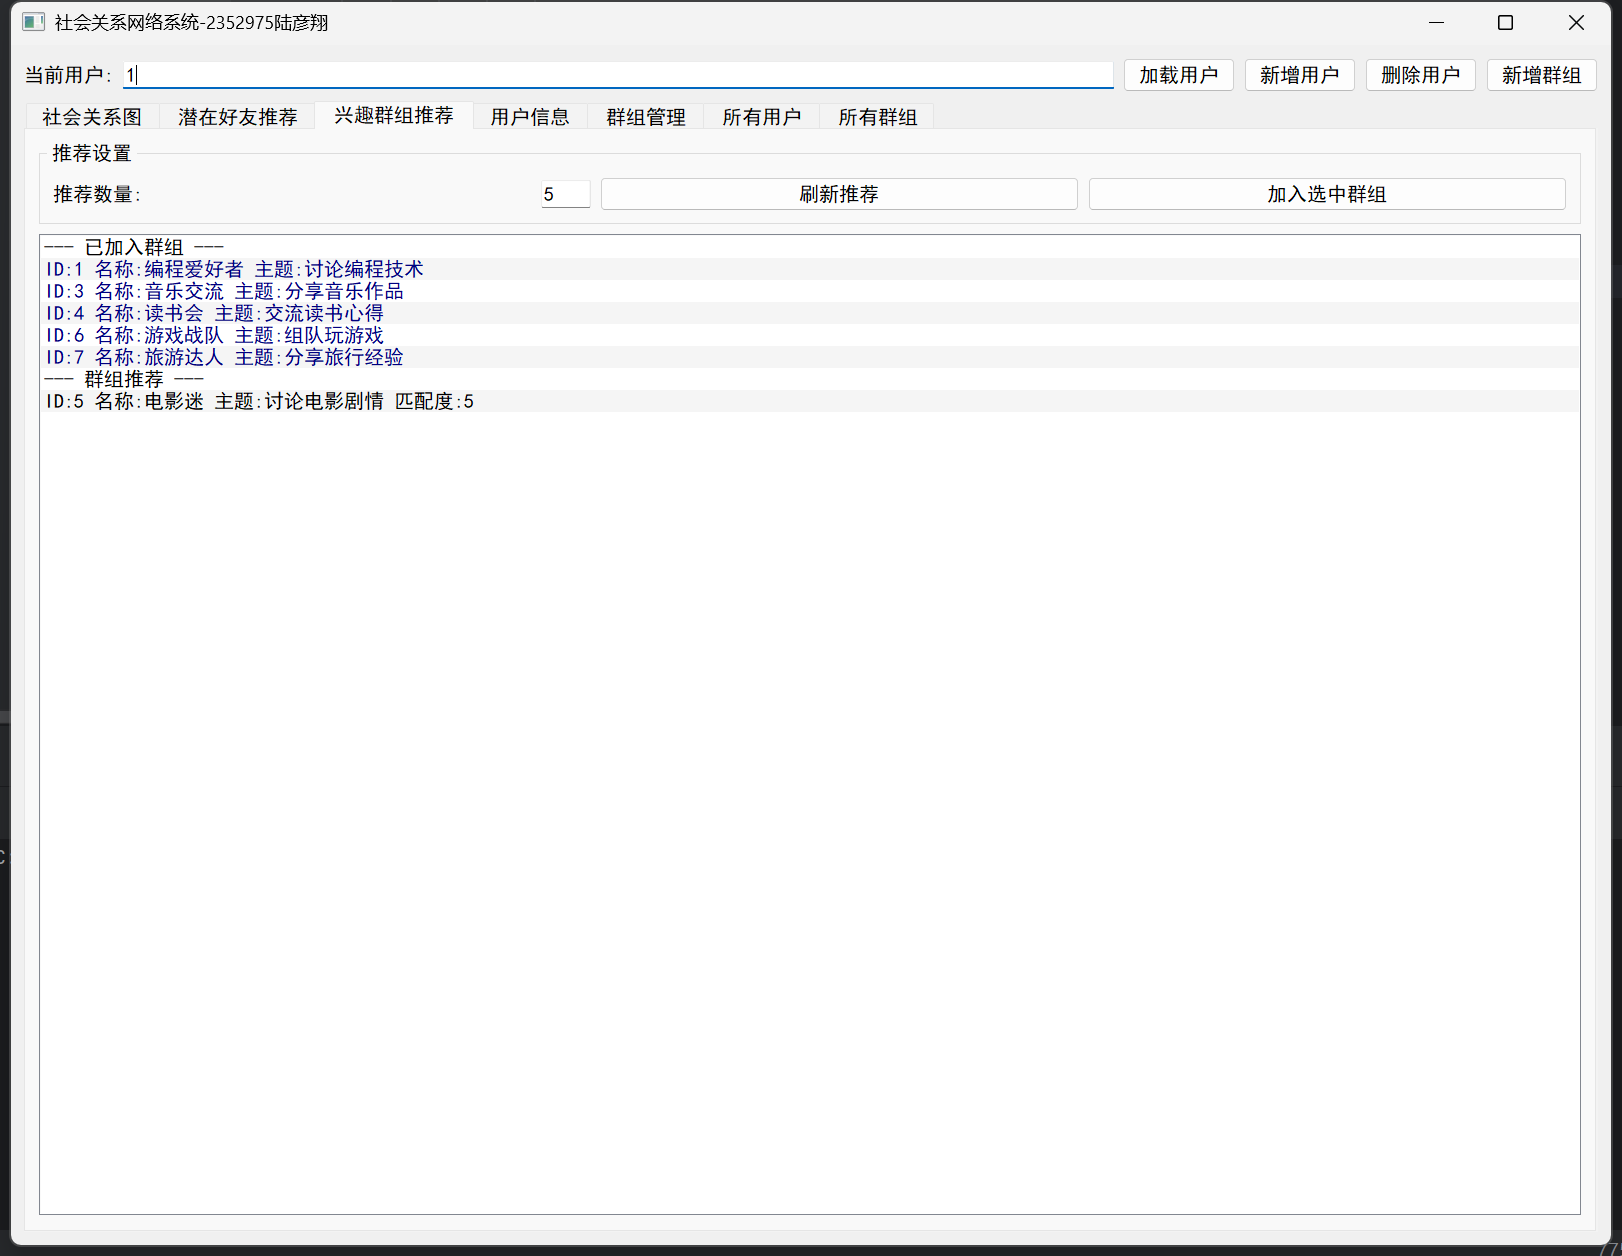
\includegraphics[width=0.5\textwidth]{pt2-4.png}
    \caption{显示已加入的群组和推荐群组}
\end{figure}

\noindent\textbf{实现方式:}

想要实现群组推荐,首先是要找出匹配度最高的群组,我在recommend\_groups函数中通过用户属性和群组标签的匹配进行匹配度计算,匹配度不为0的群组会参与推荐排序,最终根据排序结果选择分数最高的选项。

\small\begin{verbatim}
def recommend_groups(self, user_id, limit=5):
    target_user = self.network.users.get(user_id)
    if not target_user:
        return []
    if not target_user.hobbies:
        return []
    all_groups = self.network.get_all_groups()
    unjoined_groups = [group for group in all_groups if group.group_id not in 
target_user.groups]

    recommended_groups = []
    for group in unjoined_groups:
        match_point = 0
        match_point = len(target_user.hobbies & group.tags) * 5 + 5 * 
len(target_user.school & group.tags) + 5 * len(target_user.workplace & group.tags)
            
        if match_point > 0:
            recommended_groups.append({"group_id":group.group_id, 
"name":group.name, "topic":group.topic, "tag":group.tags, "match_point":match_point})
        
        return sorted(recommended_groups,key=lambda x: x["match_point"], 
reverse=True)[:limit]
\end{verbatim}

同时为了管理用户和群组之间的关系,在当前页面中还调用了join\_group函数来选择加入或者退出当前群组,这一部分内容的修改同样也会同步到关系网的绘制界面中。

\subsubsection{用户与群组信息管理}

\noindent\textbf{功能描述:}

分别设置两个页面用于显示当前加载的用户的详细信息,包括姓名,地区,学校,工作单位,爱好,其中多余多值信息需要用逗号分隔方可正确识别。操作者可以在这一界面直接进行信息的更改,点击最下方的保存按钮即可更新相关信息。

\begin{figure}[H]
    \centering
    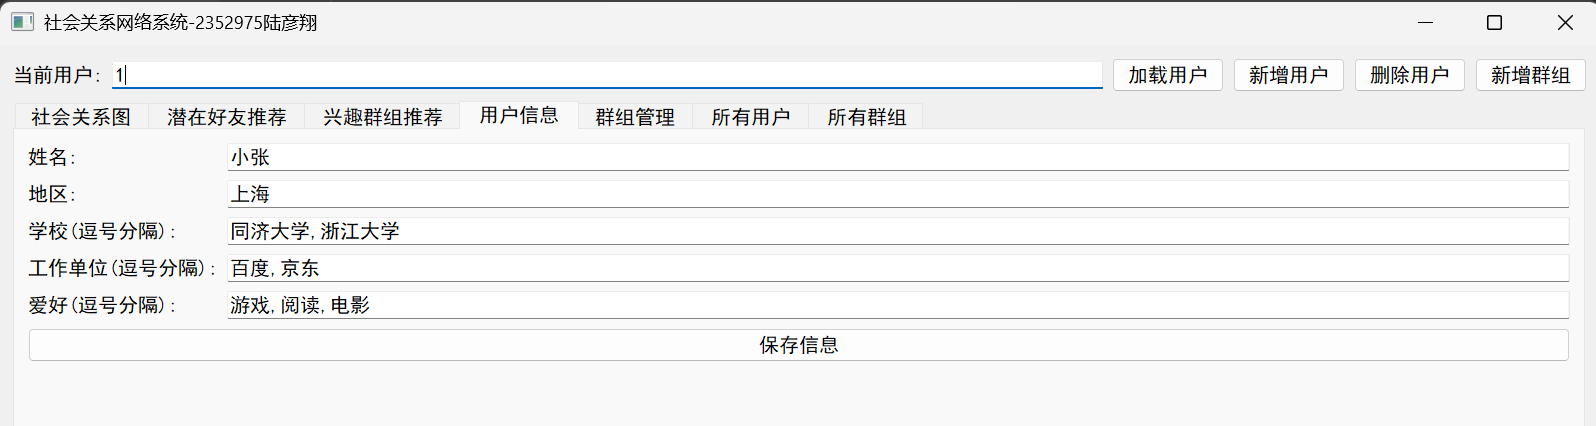
\includegraphics[width=0.5\textwidth]{pt2-5.png}
    \caption{用户信息管理界面}
\end{figure}

在群组信息管理中,由于之前没有设置过加载群组的渠道,所以我们可以在这里加载群组并且编辑其标签,名称,主题,点击保存按钮即可更新。同时,在最下方的输出框中还会输出加入了这个群组的用户,方便进行群组管理。由于在其他地方没有设置删除群组的操作,此处点击删除按钮即可将当前加载的群组进行删除。

\begin{figure}[H]
    \centering
    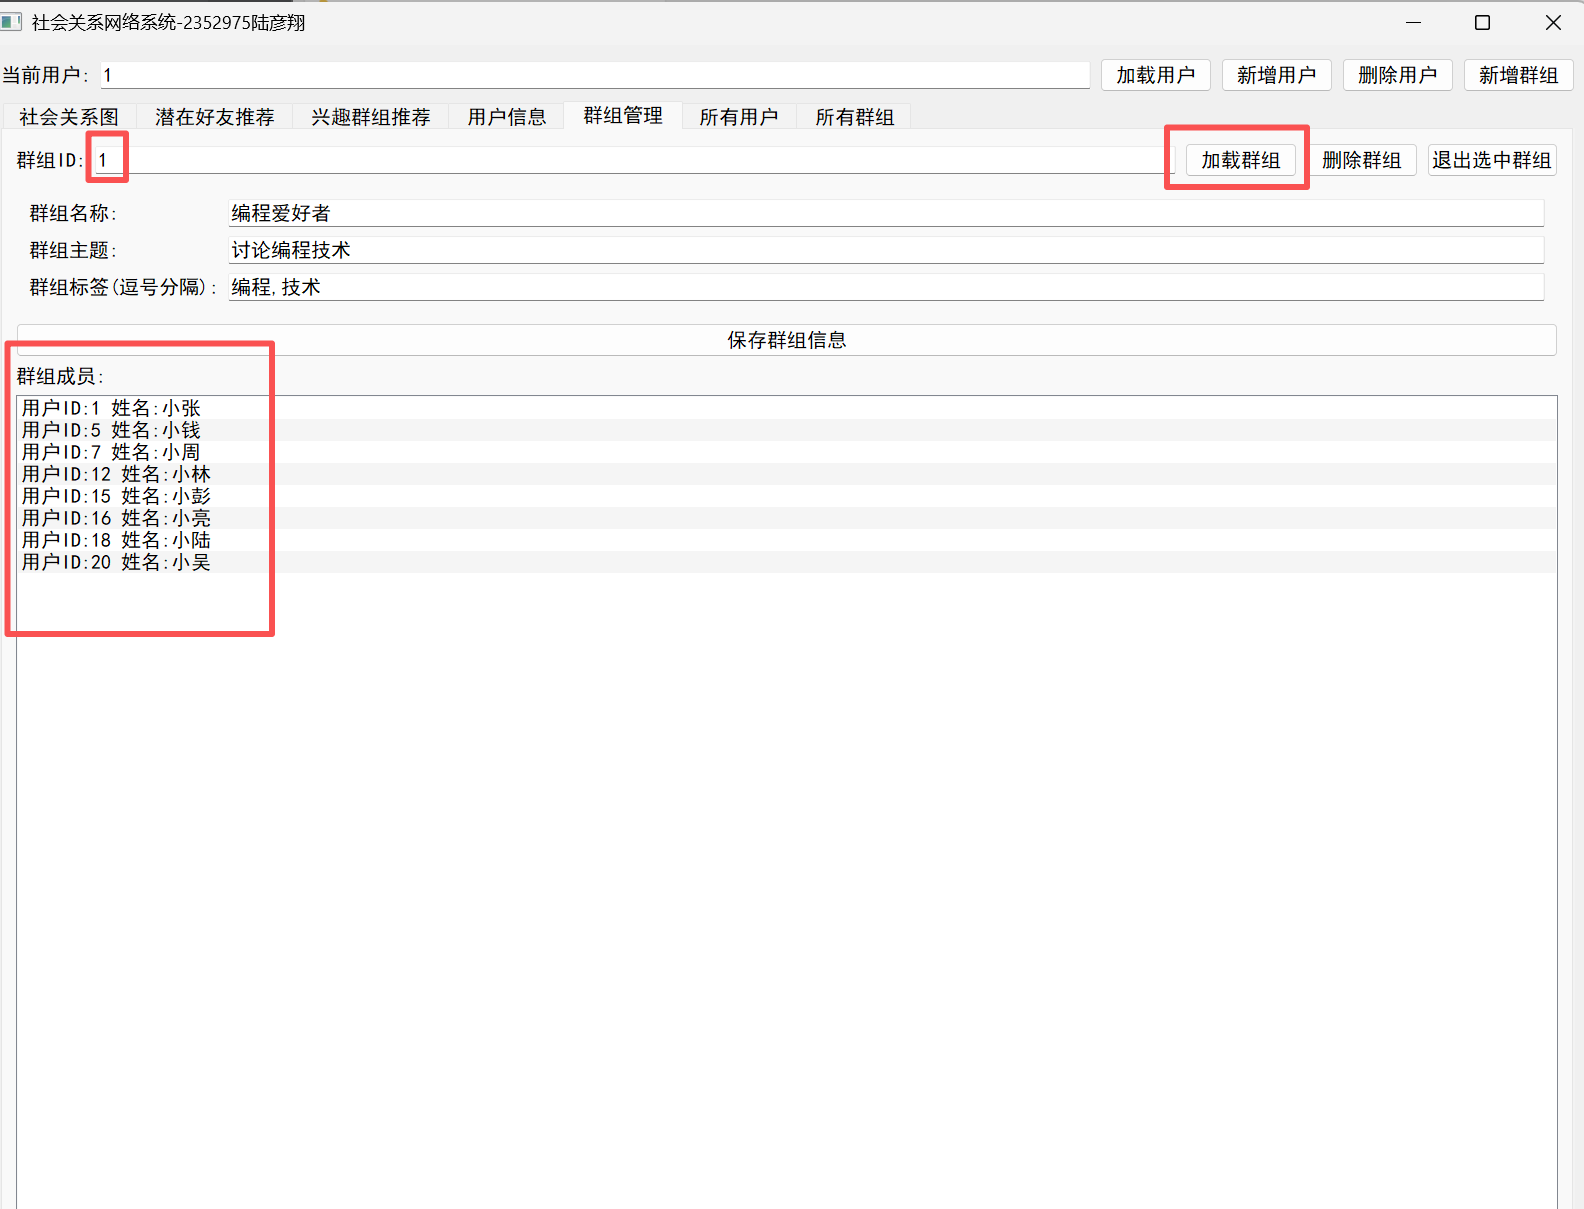
\includegraphics[width=0.5\textwidth]{pt2-6.png}
    \caption{加载群组后进入当前群组管理界面}
\end{figure}

\noindent\textbf{实现方式:}

我用了User和Group类来封装用户和群组的基本属性与行为,使用SocialNetwork来管理用户和群组的生命周期,同时设置相关函数使得删除用户之后,ID可以被回收利用。最后使用MainWindow类中的对话框和表单控制件来接收输入。

\subsubsection{用户与群组全局浏览}

\noindent\textbf{功能描述:}

为了从全局查看当前系统中究竟有哪些用户和群组,我设置两个单独的窗口,分别用于用户和群组信息的整体浏览。在全局群组管理中,也可以为当前的加载用户选定群组并加入。这些信息的排序都是依照其ID进行,由小到大进行展示。

\begin{figure}[H]
    \centering
    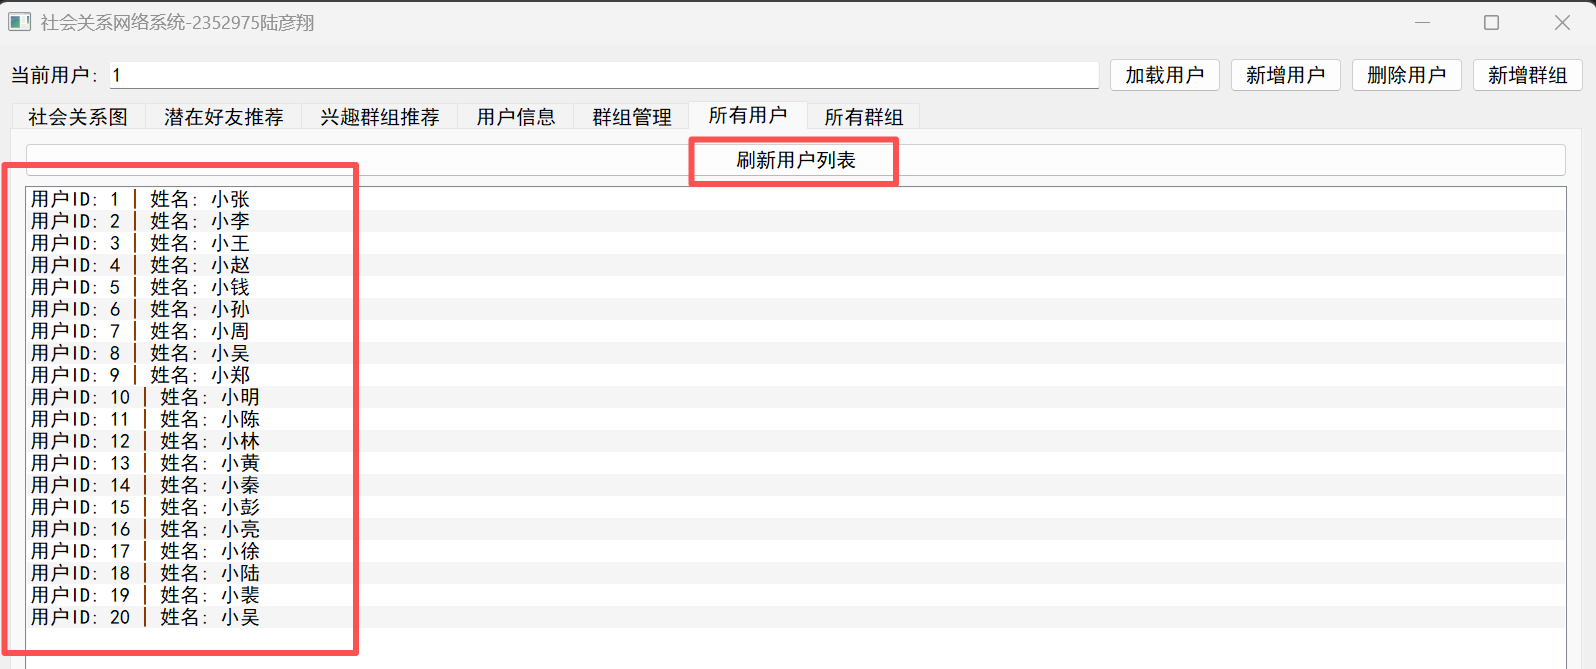
\includegraphics[width=0.5\textwidth]{pt2-7.png}
    \caption{点击刷新来获取按照ID排序的所有用户}
\end{figure}

\begin{figure}[H]
    \centering
    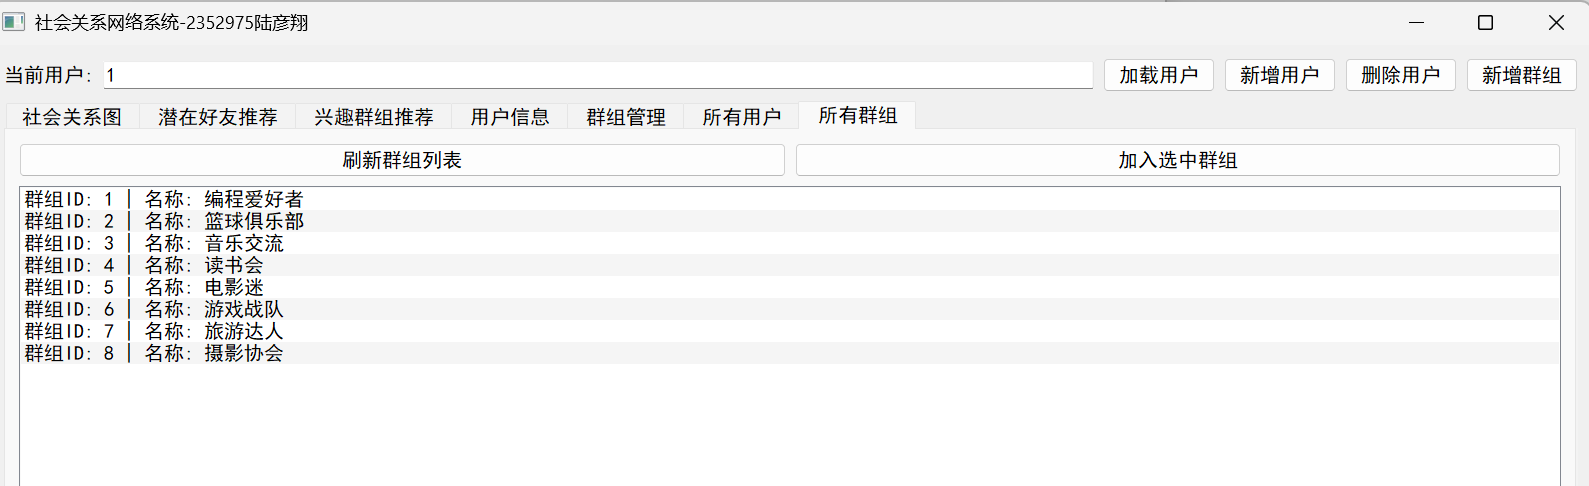
\includegraphics[width=0.5\textwidth]{pt2-8.png}
    \caption{获取所有群组列表}
\end{figure}

\noindent\textbf{实现方式:}

在SocialNetwork类中,设置get\_all\_user函数以及get\_all\_groups函数,通过遍历的方式来获取全部数据。使用QListWidget进行列表展示,同时为群组页面单独设置了一个join\_selected\_group\_from\_all函数来实现从全局列表中加入群组的功能。

\subsubsection{用户搜索}

\noindent\textbf{功能描述:}

在后期优化时发现,仅有潜在好友推荐可能会导致新导入用户缺乏信息基础,无法推荐到好友的问题,没有精确搜索功能也确实不符合关系网络模型的使用场景。因此我在潜在还有推荐界面新增了好友搜索添加功能,用户可以通过搜索联系人ID,名称的方式来进行搜索添加。由于用户的名称是一个非独特数值,可能出现重名的情况,所以这里我会先输出搜索列表再通过选择进行添加。在这一部分内容中,我也同样使用了不同颜色来表示已添加好友和未添加的搜索结果,这样看起来会更清楚。

\begin{figure}[H]
    \centering
    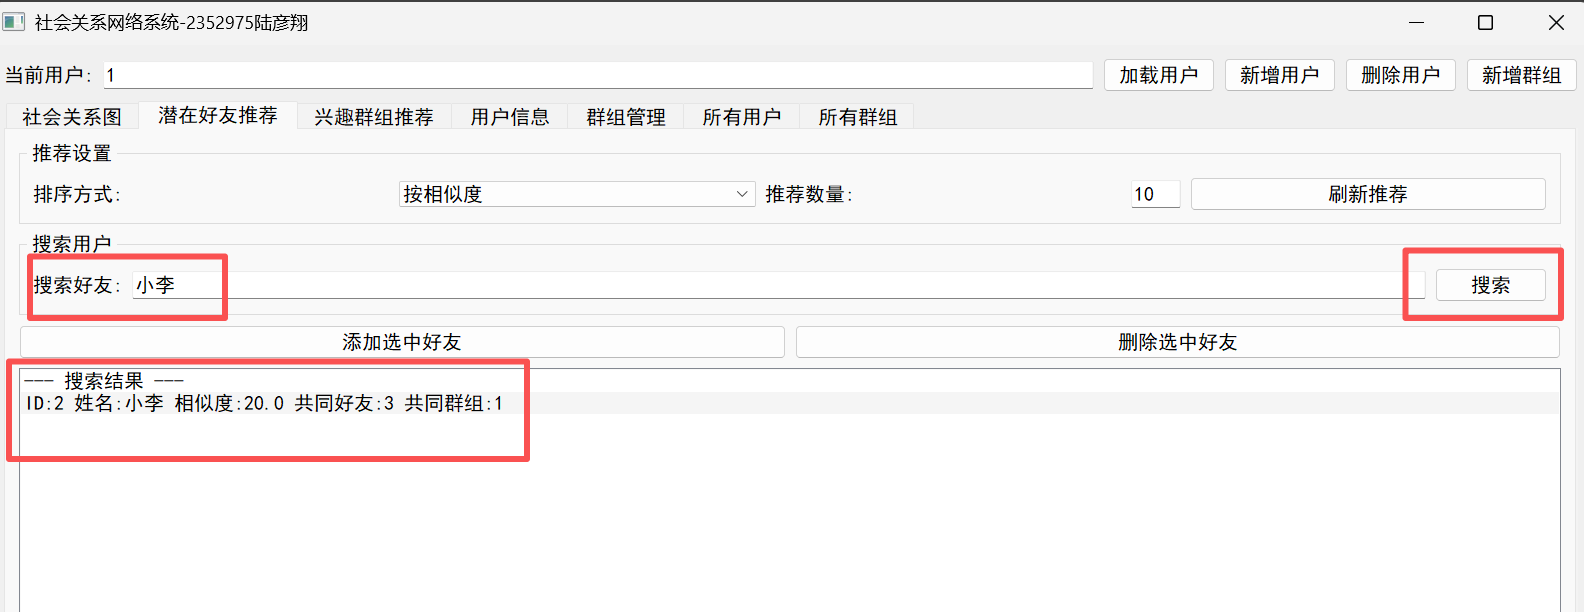
\includegraphics[width=0.5\textwidth]{pt2-9.png}
    \caption{搜索用户并操作}
\end{figure}

\noindent\textbf{实现方式:}

构建search\_friends函数进行ID和姓名的模糊搜索,然后再调用之前的显示函数在列表中展示搜索结果。

\subsubsection{测试数据初始化}

\noindent\textbf{功能描述:}

这一部分内容实际上是为当前项目内置了一个数据集,使得直接运行,不用添加用户信息即可进行测试。同时,为了增加测试的多样性,我设置了数据集和随机函数,使得每个用户拥有随机的属性,在每次生成时都会生成20个用户和8个兴趣群组。

\noindent\textbf{实现方式:}

使用init\_test\_data函数,随机生成测试数据,默认加载第一个用户便于直接开始测试。

\subsection{设计思想}

在设计本次社会关系网络系统的过程中,我采用了面向对象的设计思想,将系统的各个功能模块抽象为不同的类,以便进行高效的数据管理和可视化展示。同时,我也继续沿用了MVC设计模式,以更好地组织和分离系统的不同层次。下面是本次设计思路和核心要点:

\subsubsection{类的设计与抽象}

以下类组成了当前社交网络的组织和管理

\noindent\textbf{1.User类}

用户类,用于存储用户的基本信息,表示单个用户,包含了以下属性:ID,姓名,地区,学校,工作单位,爱好,好友,加入的群组。该类提供了添加和删除各种属性的方法,封装了用户数据操作。

\noindent\textbf{2.Group类}

群组类,用于存储群组信息,表示单个群组,包含以下属性:ID,名称,主题,标签,成员列表。这个类封装了群组数据的操作,用于管理群组成员。

\noindent\textbf{3.SocialNetwork类}

SocialNetwork表示整个社交网络,用于管理所有用户和群组的生命周期。在这个类中,我使用了字典结构存储用户和群组信息。同时,在这里面还实现了ID的自动分配和回收机制,防止系统长期运行之后出现的ID浪费情况。

\noindent\textbf{4.SocialNetworkLogic类}

这个类时整个系统的核心逻辑层,实现了社交网络的各种算法和业务逻辑,包括相似度计算,好友推荐,群组推荐,社交关系图构建等。

\noindent\textbf{5.SocialGraphWidget类}

该类继承自QWidegt类,作为社交网络可视化组件,用于绘制以用户社交关系图,实现了节点的自动布局,缩放和平移功能,便于用户在主界面上查看当前加载用户和其他用户以及群组之间的关系。

\noindent\textbf{6.MainWindow类}

主窗口类,负责构建整个应用程序的用户界面并处理用户交互。该类通过多个标签页来划分整个系统的功能,实现了系统功能的闭环。

\subsubsection{数据结构的选择}

在设计整个项目时,我主要使用了以下三种数据结构:集合、字典和列表。

对于集合(set)的应用,用户的好友列表、群组成员列表以及多值属性(学校、工作单位、爱好)均使用集合存储。这种选择便于快速查找和计算交集比如共同好友、共同群组,提高了相似度计算的效率。

对于字典(dictionary),得益于python本身对于字典的支持,在使用字典时不需要像c++一样使用map容器,在SocialNetwork类中使用字典存储用户和群组信息,以ID作为键,实现了O(1)时间复杂度的查找操作。这种结构适合管理大量用户和群组数据。

在需要保持顺序或进行排序的场景(如推荐列表)中,我选择使用列表(list)结构,结合Python的sorted函数和lambda表达式,实现了按不同criteria的排序功能。

\subsubsection{算法介绍}

\noindent\textbf{1.相似度计算}

在calculate\_similarity方法中,采用多维度加权计算方式,考虑共同好友(30\%)、共同群组(20\%)、共同学校(15\%)、共同单位(15\%)、相同地区(5\%)和共同爱好(15\%)六个维度,通过分配不同的权重来控制各个部分的重要性。

\noindent\textbf{2.好友推荐算法}

在get\_potential\_friends方法中,首先从当前用户的好友的好友和群组成员中筛选候选用户,然后计算每个候选用户与当前用户的相似度,最后根据用户选择的排序方式(相似度、共同好友数、共同群组数)进行排序并返回取得分数最高的top-k个结果。

\noindent\textbf{3.群组推荐算法}

在recommend\_groups方法中,根据用户的属性,例如爱好、学校、工作单位,与群组标签的匹配程度计算匹配度,按匹配度排序后返回前k个推荐群组。

\noindent\textbf{4.社交关系图构建算法}

在get\_social\_graph方法中,以当前用户为中心,遍历其好友和加入的群组,构建包含节点和边的图数据结构,供可视化组件使用。

\noindent\textbf{5.节点布局算法}

在SocialGraphWidget的calculate\_node\_positions方法中,采用极坐标布局加随机扰动的方式,将当前用户置于中心,好友节点和群组节点分布在不同半径的环上,通过随机扰动避免节点重叠,一定程度上使得图像更加清晰。

\subsubsection{MVC架构划分}

在模型层面主要包含:User、Group和SocialNetwork类。

在视图层主要包含:SocialGraphWidget和MainWindow类。

在控制器层主要包含:ocialNetworkLogic类。

\subsection{逻辑结构与物理结构}

\subsubsection{逻辑结构}

\noindent\textbf{1.集合结构}

如之前部分中所说,所有采用集合进行存储的内容都可以视作集合结构,包括用户的好友关系、群组成员关系以及多值属性。

\noindent\textbf{2.图结构}

顶点:用户和群组作为图中的顶点,每个顶点都包含丰富的属性信息。

边:因为好友关系是相互的,故而用户之间的好友关系形成无向边,用户与群组之间的加入关系形成有向边,用户和群组有加入关系,而群组和用户为包含关系。

图:该图结构具有小世界特性,通过朋友的朋友关系可以快速扩展社交圈,这正体现了现实社会关系网络的特点。

\noindent\textbf{3.层次结构}

之前我们提到,系统主界面中只可以加载用户而不可以加载群组,所以我们的层次结构以用户为中心,向外扩展的中心层为加入的群组和当前好友,再向外是推荐好友和群组,最外圈是未被推荐的用户/群组。

\noindent\textbf{4.类结构}

系统采用面向对象的方式组织数据,通过类之间的关联关系构建逻辑结构:

\begin{verbatim}
    User --(多对多)--> Group
    User --(多对多)--> User
    SocialNetwork --(1对多)--> User
    SocialNetwork --(1对多)--> Group
\end{verbatim}

\subsubsection{物理结构}

在物理存储层面,本系统采用了多种数据结构来实现高效的数据管理和访问:

\noindent\textbf{1.字典存储}

在SocialNetwork类中,使用字典来存储用户和群组信息:

\begin{verbatim}
self.users = {}  # user_id -> User对象
self.groups = {}  # group_id -> Group对象
\end{verbatim}

这种存储方式提供了O(1)时间复杂度的查找效率,非常适合根据ID快速检索对象。

\noindent\textbf{2.集合存储}

对于需要快速计算交集和并集的场景,采用集合存储,集合存储确保了这些数据的唯一性,并提供了高效的交集、并集计算能力。:

\begin{verbatim}
# User类中的定义
self.friends = set()      # 好友ID集合
self.groups = set()       # 加入的群组ID集合  
self.school = set()       # 学校集合
self.workplace = set()   # 工作单位集合
self.hobbies = set()     # 爱好集合

# Group类中的定义
self.members = set()     # 成员ID集合
self.tags = set()        # 标签集合
\end{verbatim}

\noindent\textbf{3.列表存储}

在需要保持顺序或进行排序的场景中使用列表:

\begin{verbatim}
# 在SocialNetworkLogic中的推荐算法
return sorted(new_friends, key=lambda x: x["similarity_score"], reverse=True)[:limit]
\end{verbatim}

列表结构结合排序算法,实现了按不同要求的推荐功能。

\noindent\textbf{4.图数据的动态生成}

社交关系图数据并非静态存储,而是动态生成,这样可以确保社交关系图的实时更新,同时节省了存储空间:

\tiny\begin{verbatim}
    def get_social_graph(self, user_id):
        if not self.network.has_user(user_id):
            return {"nodes":[], "edges":[]}
        user = self.network.get_user(user_id)
        nodes = []
        nodes.append({"id": f"user{user_id}", "name": user.name, "type": "self"})
        edges = []
        for anyone in user.friends:
            friend = self.network.get_user(anyone)
            if friend:
                nodes.append({"id": f"user{friend.user_id}", "name": friend.name, "type": "friend"})
                edges.append({"source": f"user{user_id}", "target": f"user{friend.user_id}"})

        for anygroup in user.groups:
            group = self.network.get_group(anygroup)
            if group:
                nodes.append({"id": f"group{group.group_id}", "name": group.name, "type": "group"})
                edges.append({"source": f"user{user_id}", "target": f"group{group.group_id}"})

        return {"nodes":nodes, "edges":edges}
\end{verbatim}
\normalsize 
\noindent\textbf{5.内存管理机制}

在项目中,我设计了ID回收机制,这种机制优先重用被删除对象的ID,既提高了ID利用率,又避免了ID的无限增长:

\begin{verbatim}
self.recycled_user_ids = set()  # 存储已删除的用户ID
self.recycled_group_ids = set() # 存储已删除的群组ID
\end{verbatim}

\noindent\textbf{6.可视化数据临时存储}

在可视化组件中,使用字典临时存储节点位置信息,这种存储方式便于在绘制过程中快速查找节点位置,提高了渲染效率:

\begin{verbatim}
self.node_positions = {}  # 节点ID -> 位置坐标
\end{verbatim}

\subsection{开发平台}

计算机型号:华硕ROG枪神7

计算机内存:32GB

CPU:13th Gen Intel(R) Core(TM) i9-13980HX

操作系统:Windows11专业版

开发语言:python3.12

开发框架:PyQt5

开发环境:PyCharm 2025.2.0.1

运行环境:

PyQt5==5.15.11

PyQt5-Qt5==5.15.2

PyQt5\_sip==12.17.0

PySide6\_Addons==6.9.1

PySide6\_Essentials==6.9.1

setuptools==78.1.1

shiboken6==6.9.1

wheel==0.45.1

\subsection{运行说明}

运行方法:
\begin{verbatim}
    pip install 
    PyQt5==5.15.11
    PyQt5-Qt5==5.15.2
    PyQt5_sip==12.17.0
    PySide6_Addons==6.9.1
    PySide6_Essentials==6.9.1
    setuptools==78.1.1
    shiboken6==6.9.1
    wheel==0.45.1
    python main_window.py
\end{verbatim}

或者在pycharm中运行main\_window.py即可

\subsection{系统运行结果分析说明}

下面我将逐步展示这个系统的运行结果。

首先打开界面,系统根据内置的数据库和随机生成的个人信息,加载ID为1的用户并显示其关系网络。

\begin{figure}[H]
    \centering
    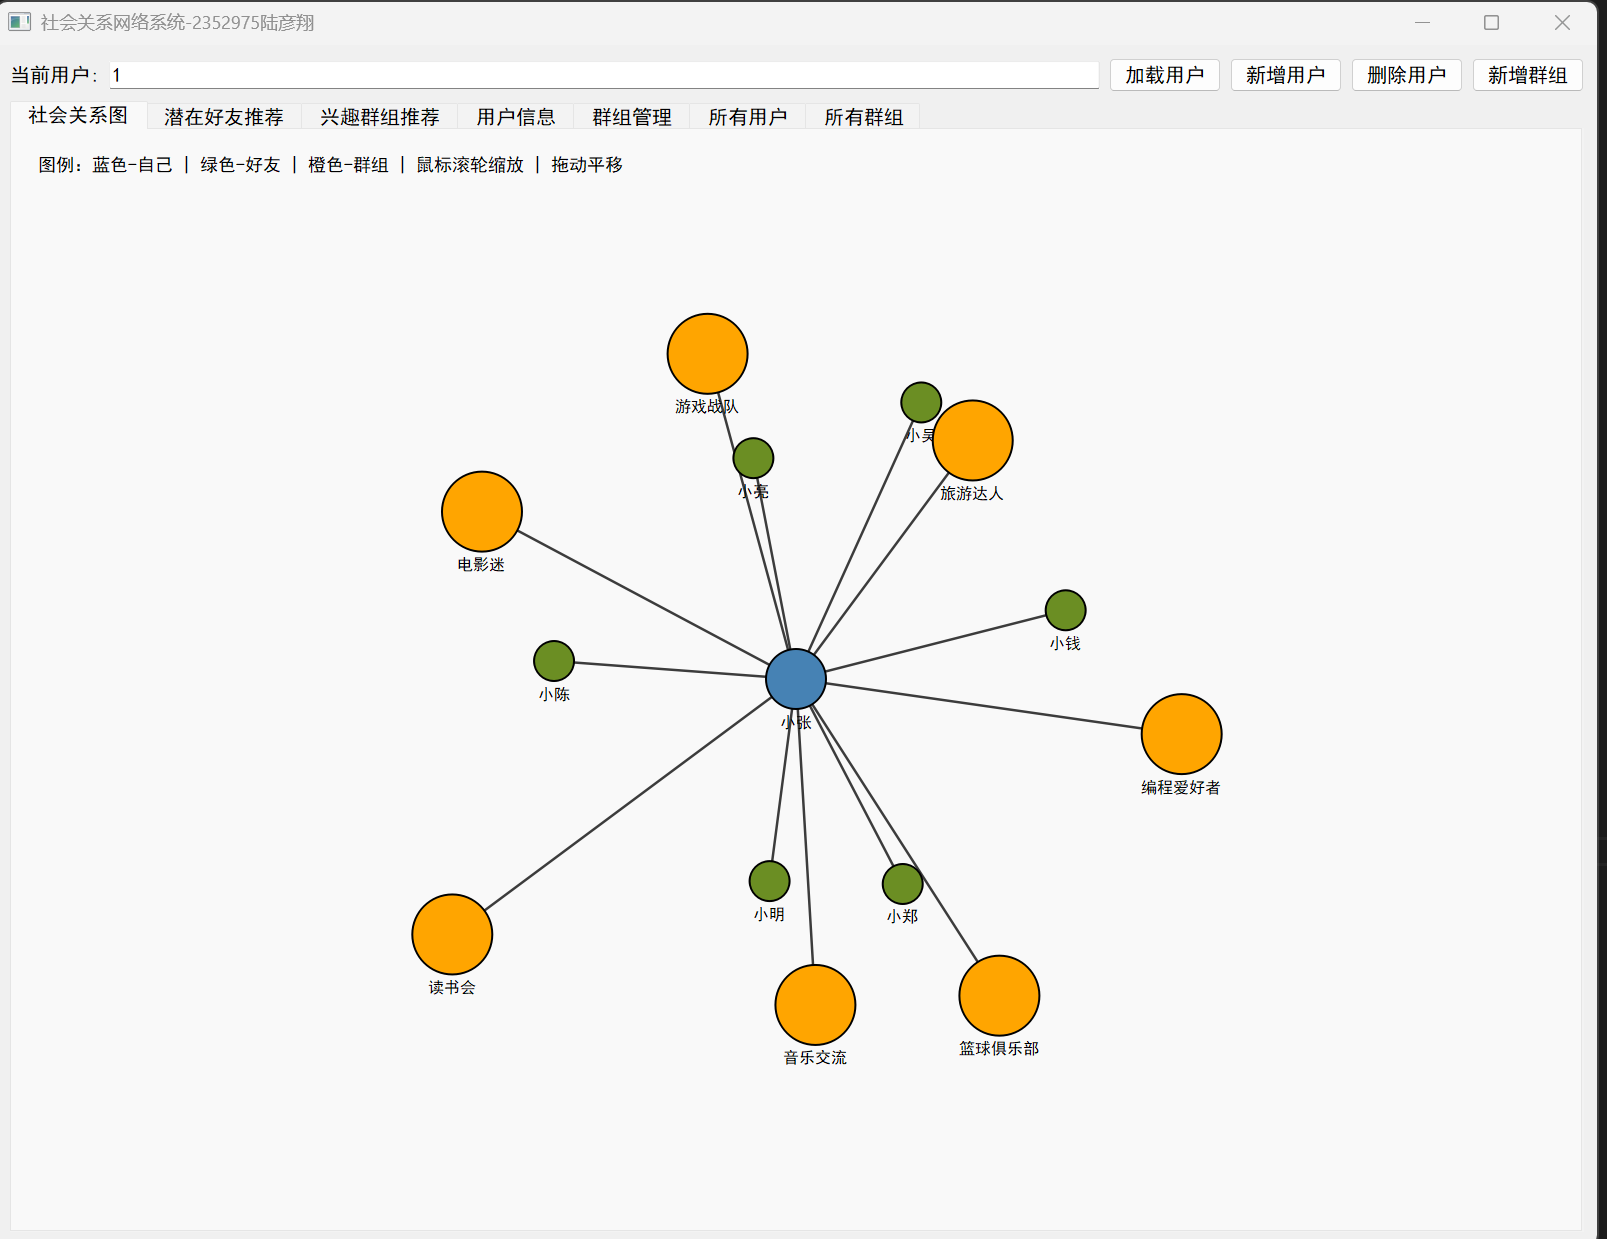
\includegraphics[width=0.5\textwidth]{pt2-10.png}
    \caption{加载默认用户并显示关系图}
\end{figure}

在输入框中输入其他用户的ID,再点击加载按钮即可加载到其他用户,并且更新视图。

\begin{figure}[H]
    \centering
    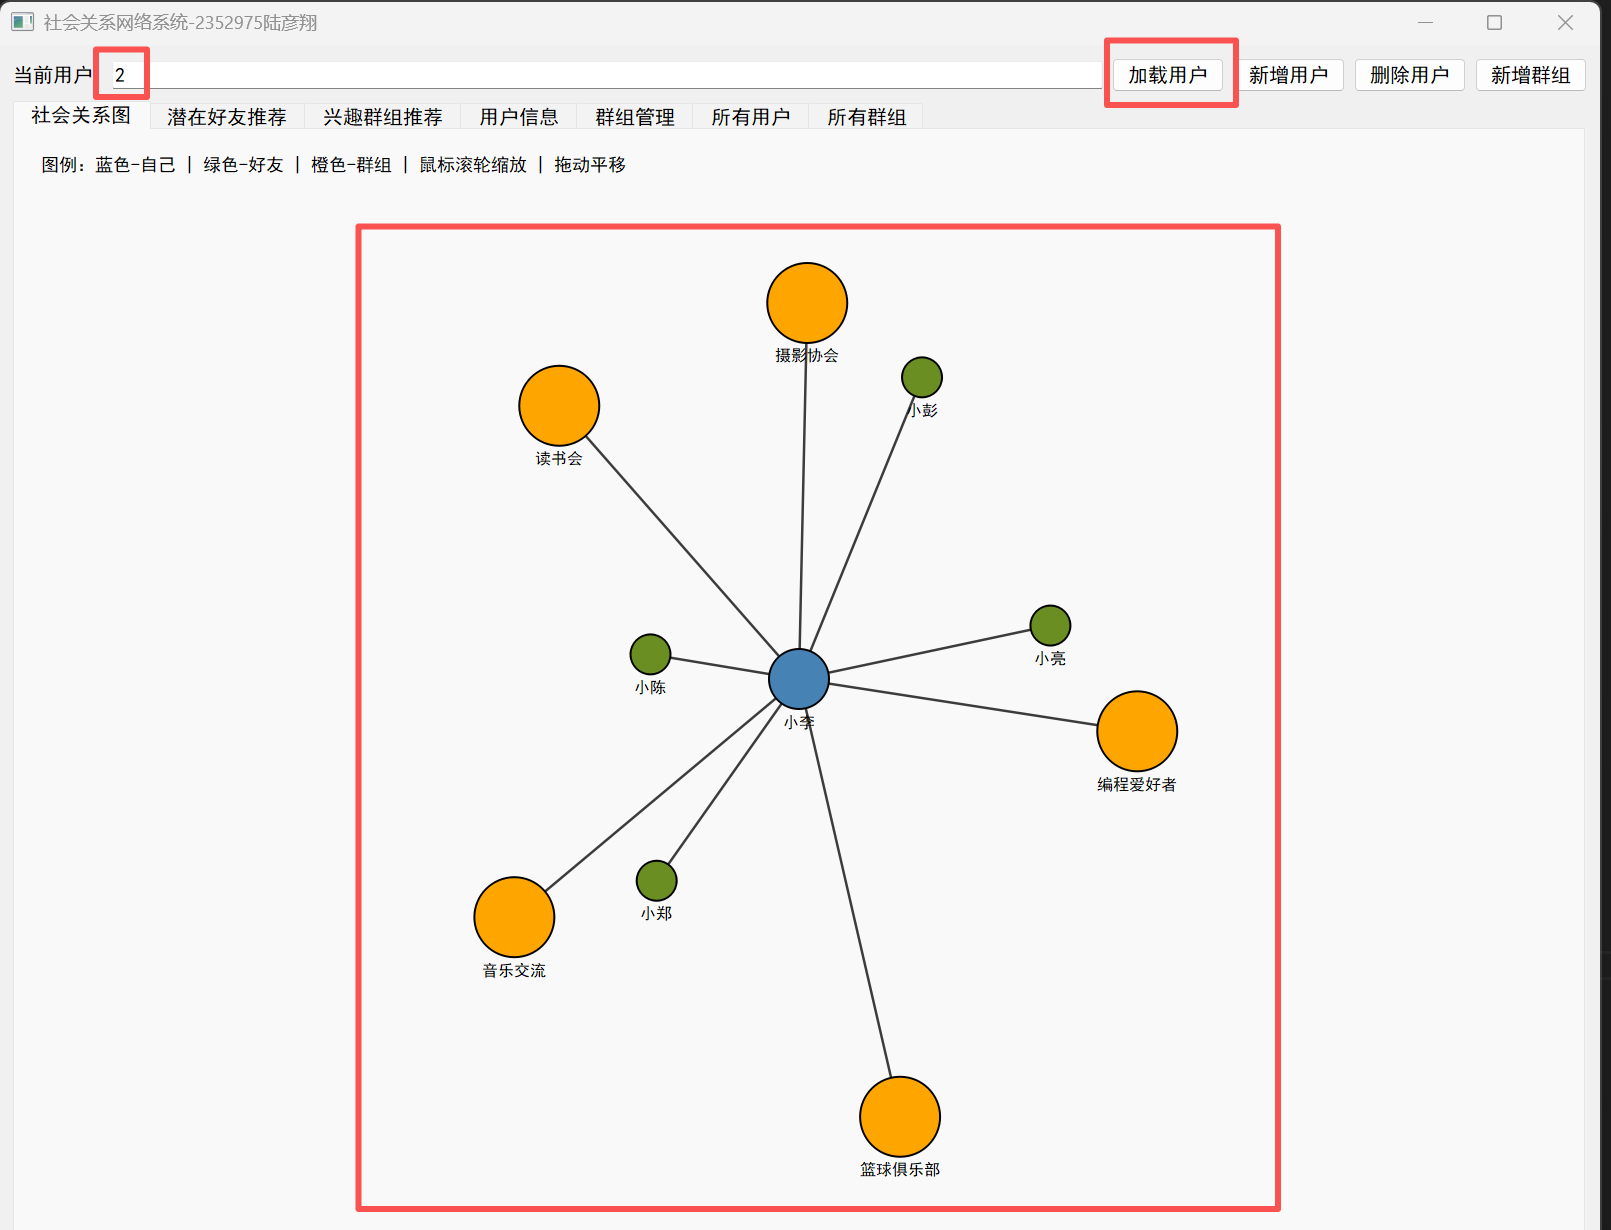
\includegraphics[width=0.5\textwidth]{pt2-11.png}
    \caption{更新加载对象}
\end{figure}

如果视图绘制的不清楚,可以再点击一次加载,即可尝试重新绘制。

\begin{figure}[H]
    \centering
    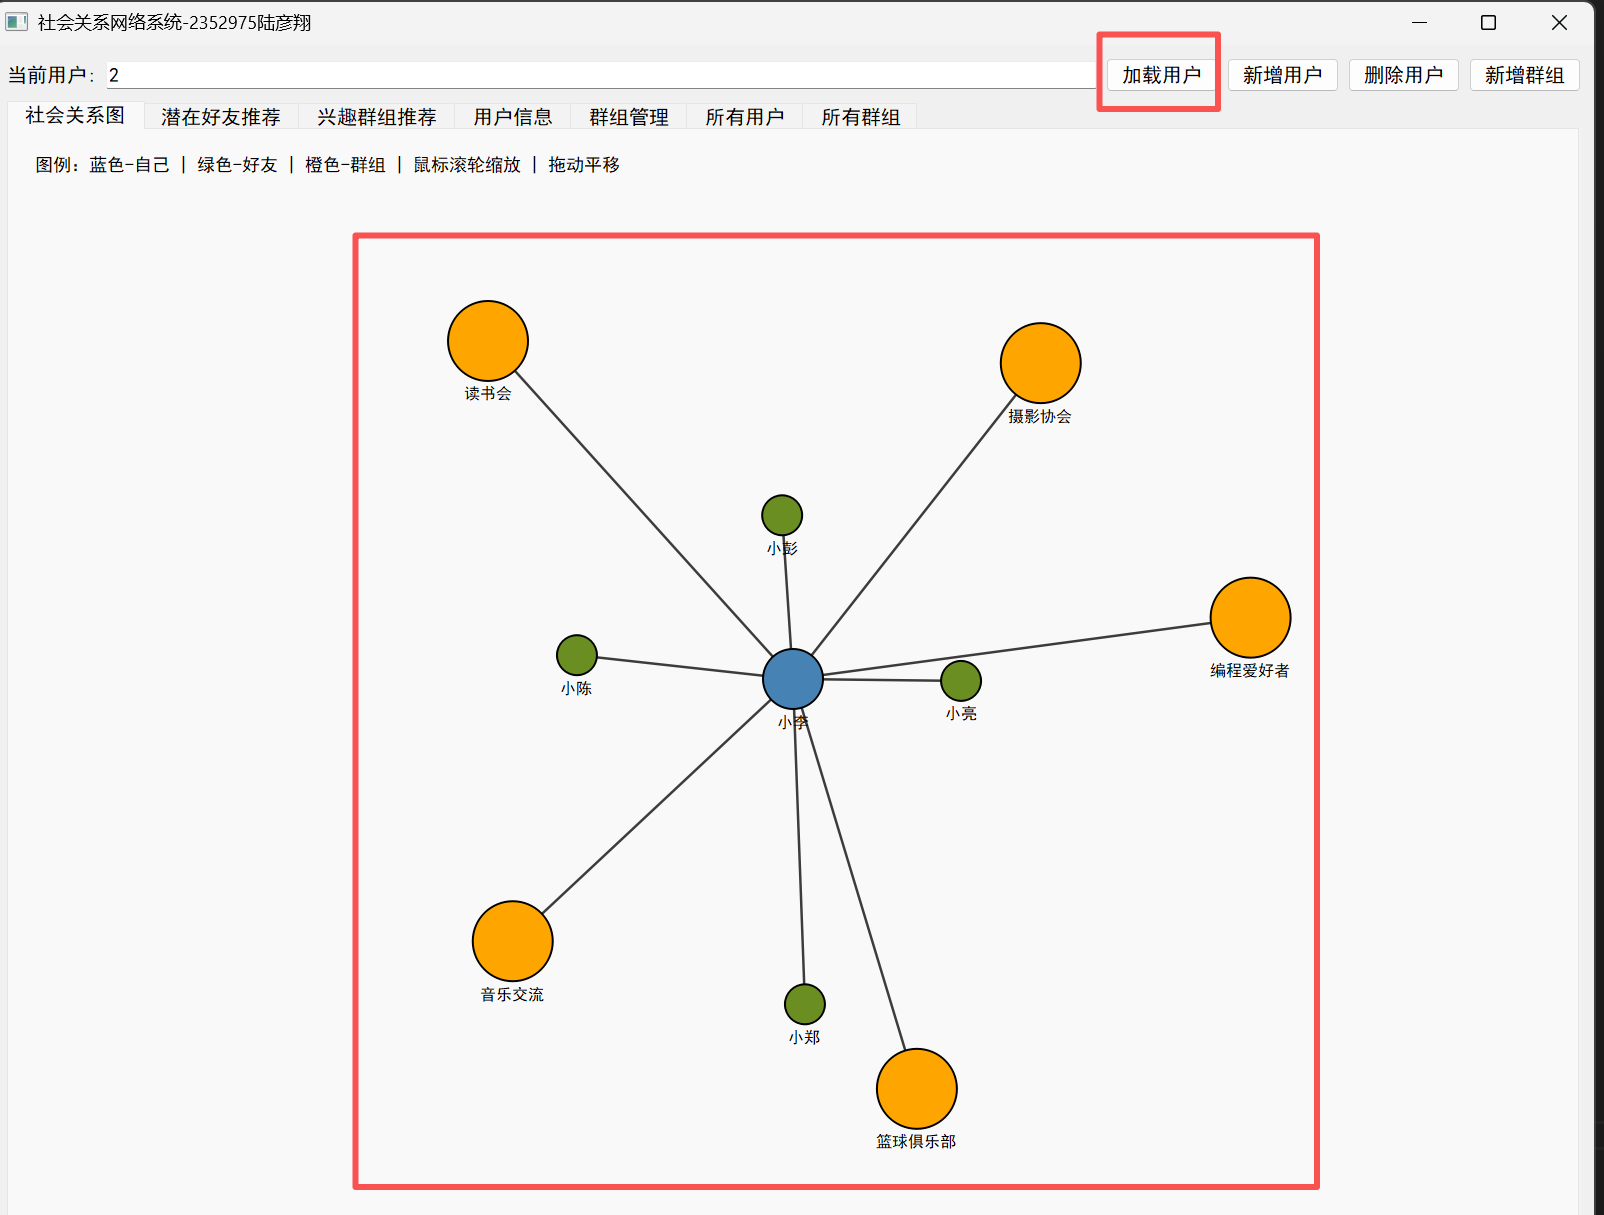
\includegraphics[width=0.5\textwidth]{pt2-12.png}
    \caption{再一次加载可以更新视图}
\end{figure}

加载错误用户会显示用户不存在,操作对象保留为上一个加载的用户。

\begin{figure}[H]
    \centering
    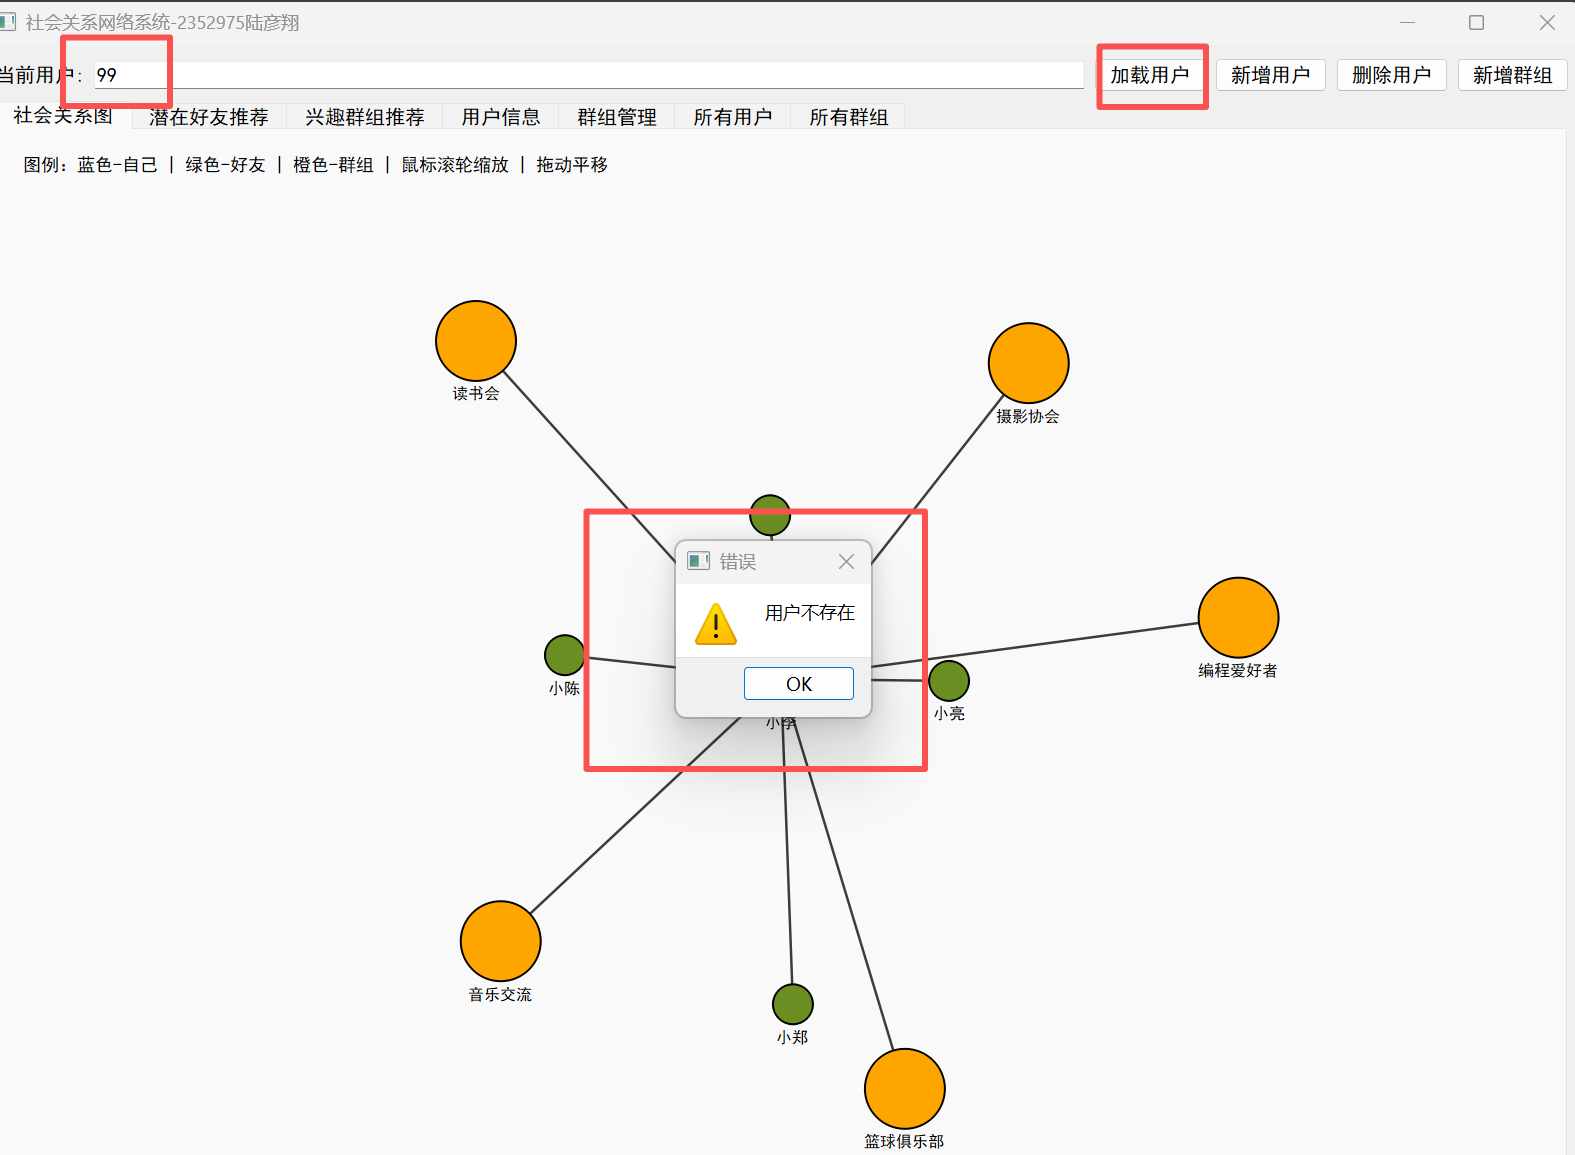
\includegraphics[width=0.5\textwidth]{pt2-13.png}
    \caption{错误用户加载}
\end{figure}

进入潜在好友推荐界面,默认按照相似度进行排序,推荐10个好友。

\begin{figure}[H]
    \centering
    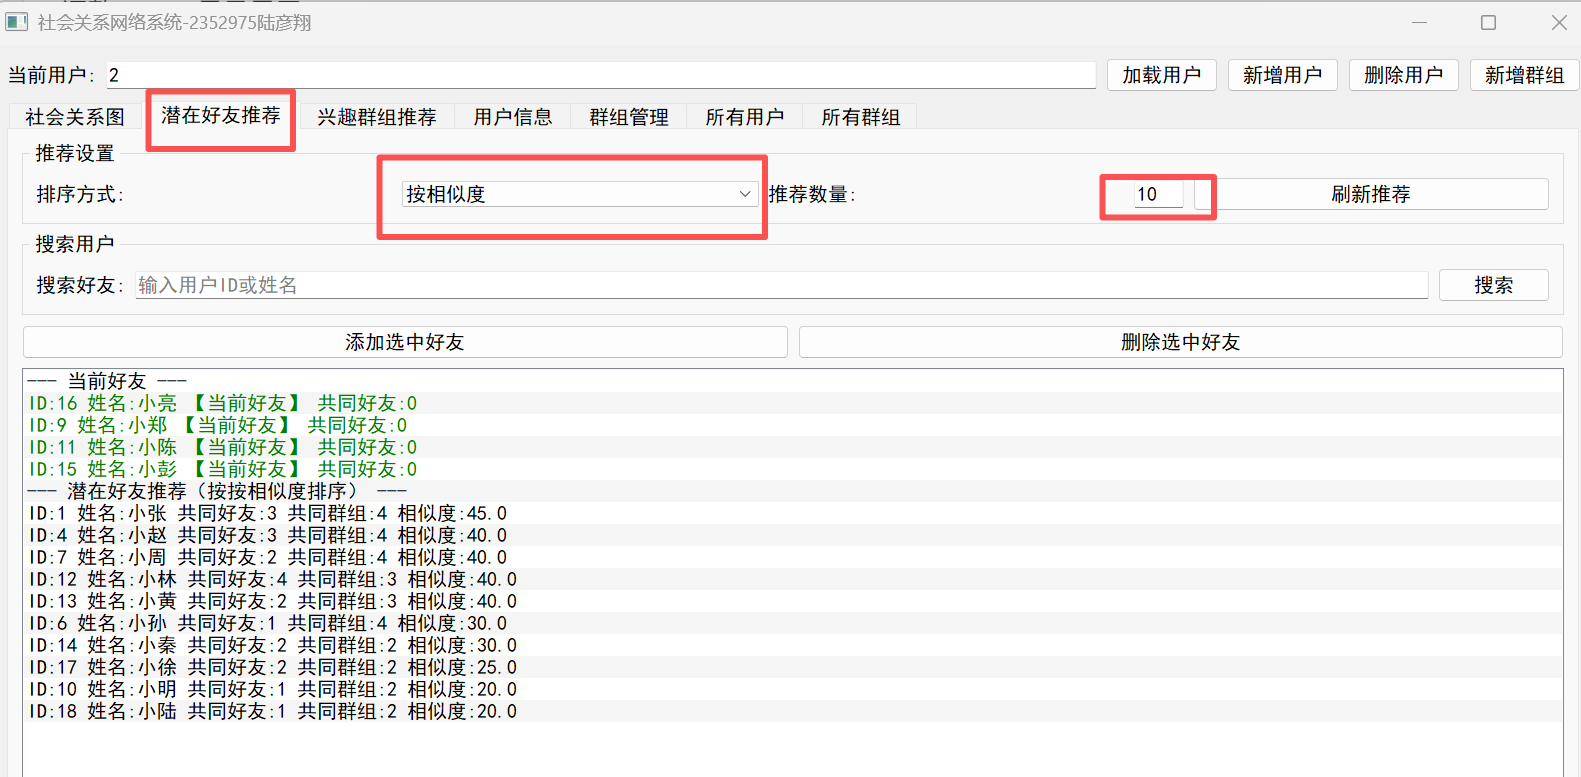
\includegraphics[width=0.5\textwidth]{pt2-14.png}
    \caption{默认推荐界面}
\end{figure}

可以更改推荐排血方式和推荐人数

\begin{figure}[H]
    \centering
    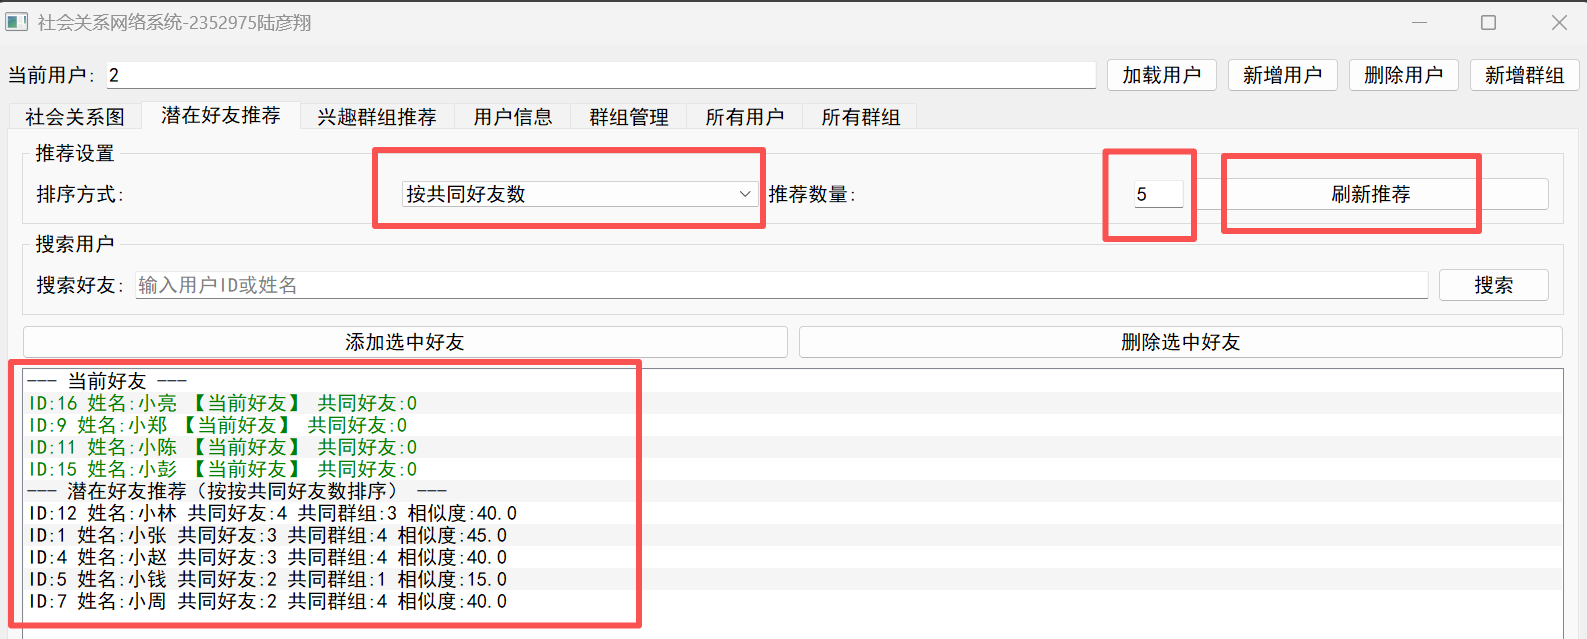
\includegraphics[width=0.5\textwidth]{pt2-15.png}
    \caption{按照共同好友推荐5个}
\end{figure}

\begin{figure}[H]
    \centering
    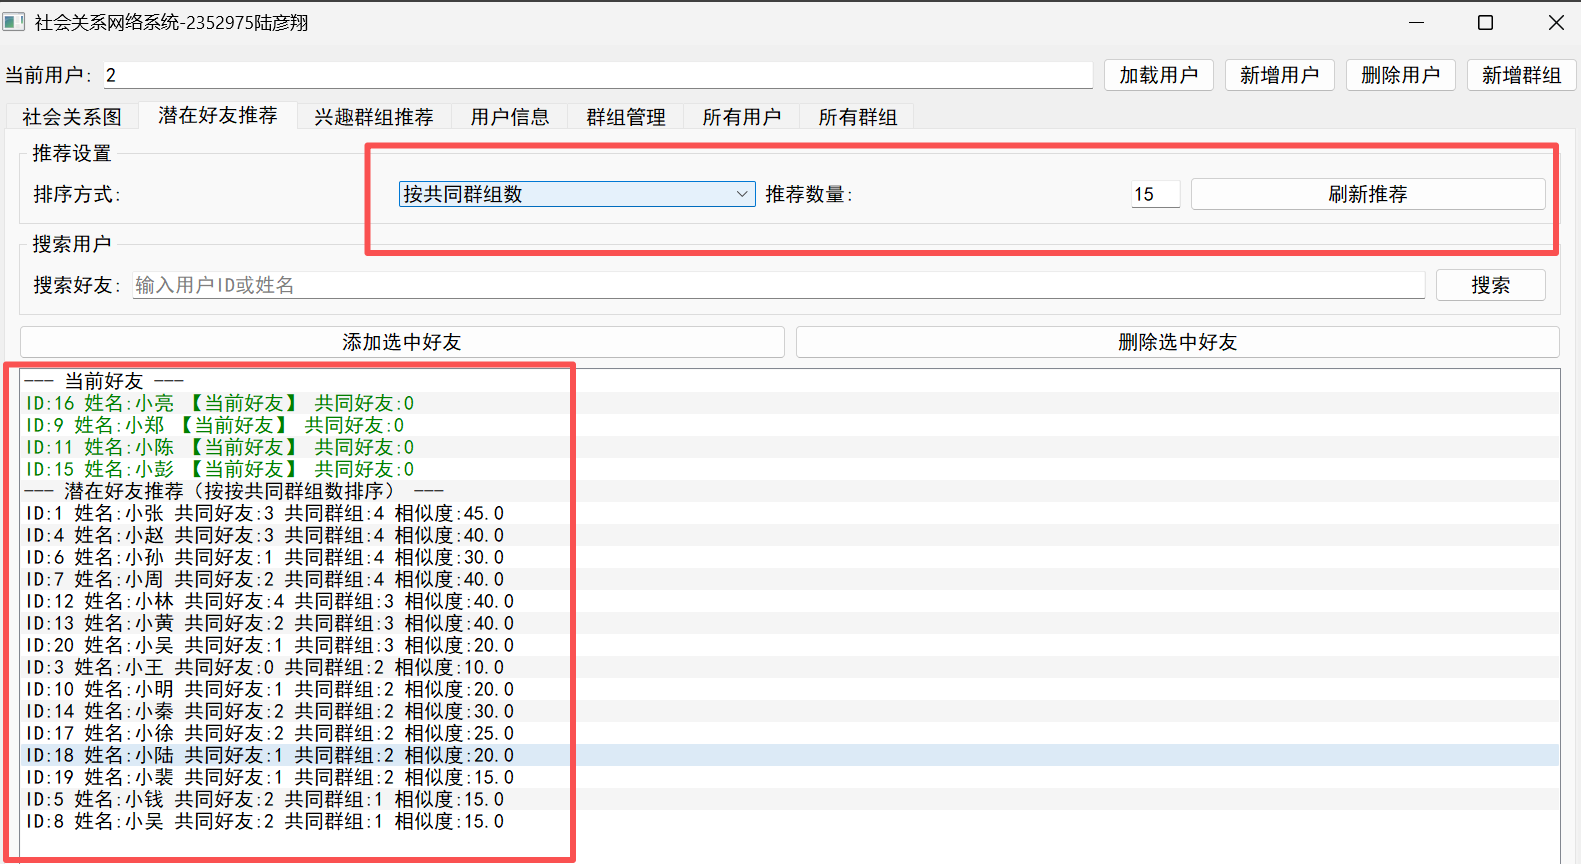
\includegraphics[width=0.5\textwidth]{pt2-16.png}
    \caption{按照共同群组数量推荐15个}
\end{figure}

在添加好友,删除好友之后,推荐结果(分数)也会随之发生改变,个人社交网络图也会进行更新。

\begin{figure}[H]
    \centering
    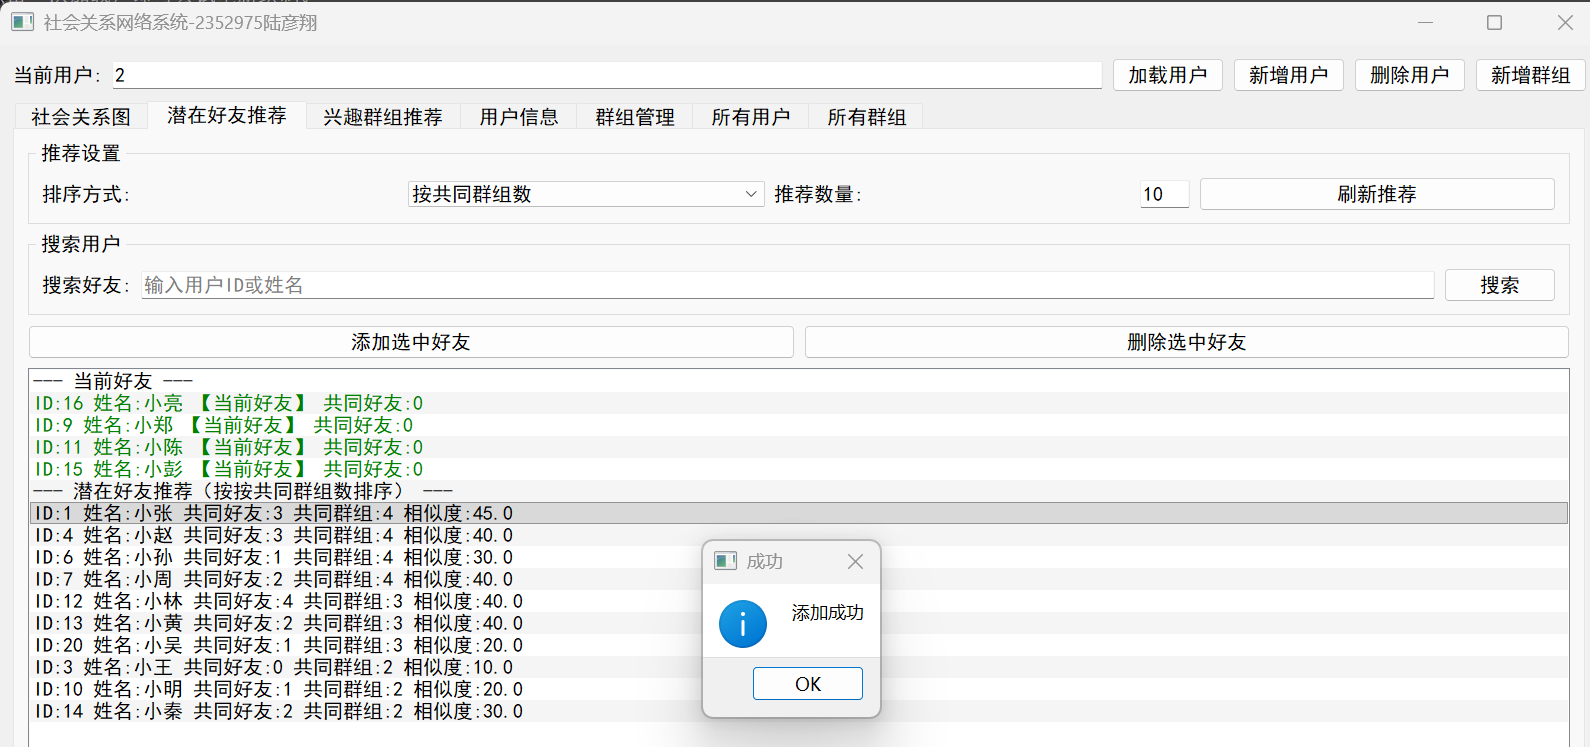
\includegraphics[width=0.5\textwidth]{pt2-17.png}
    \caption{添加新朋友}
\end{figure}

\begin{figure}[H]
    \centering
    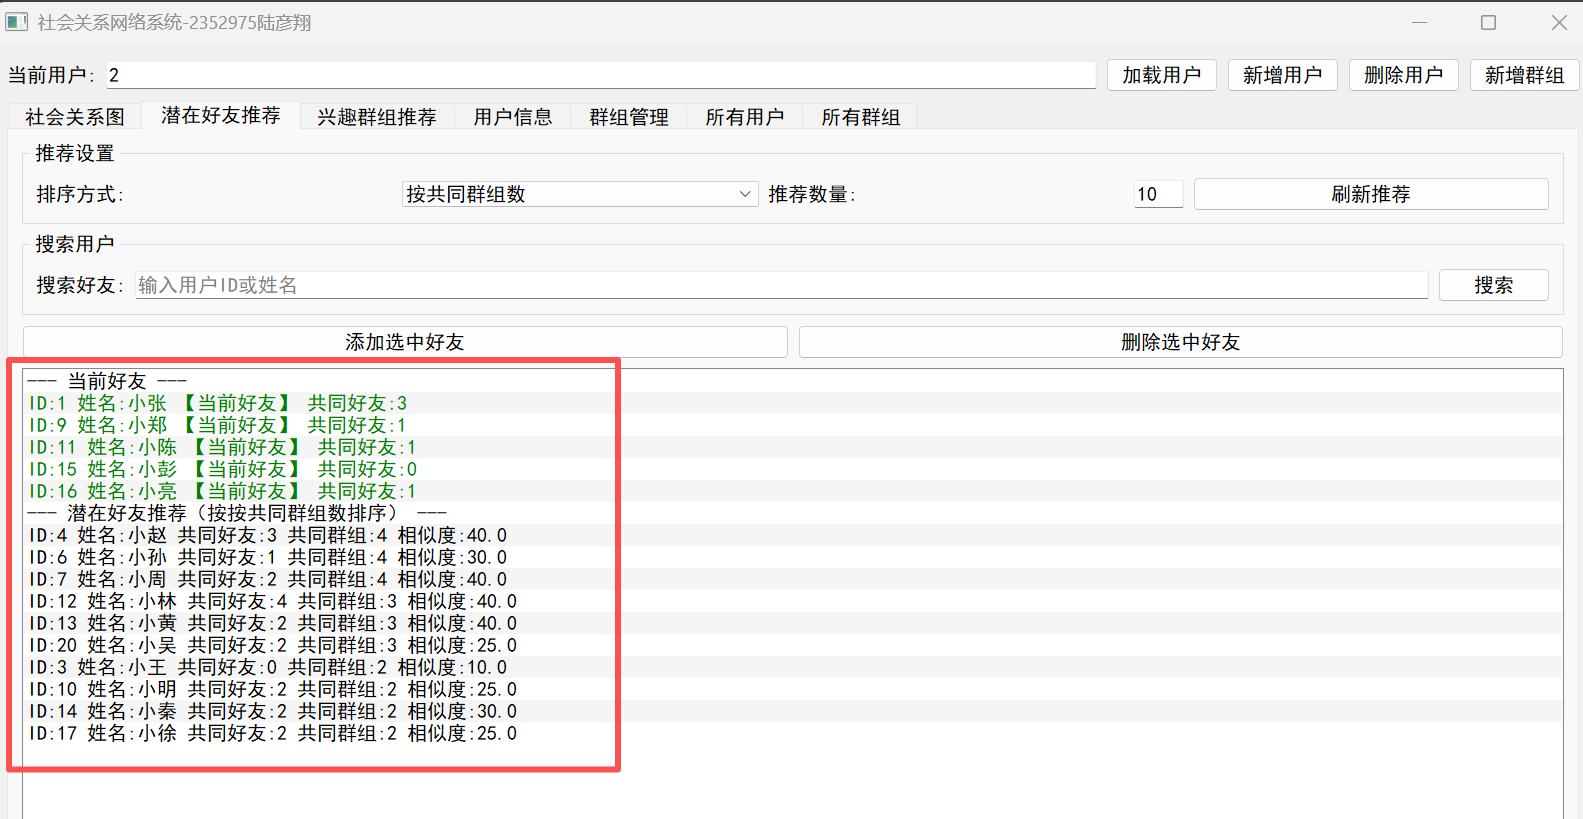
\includegraphics[width=0.5\textwidth]{pt2-18.png}
    \caption{推荐结果发生更新}
\end{figure}

\begin{figure}[H]
    \centering
    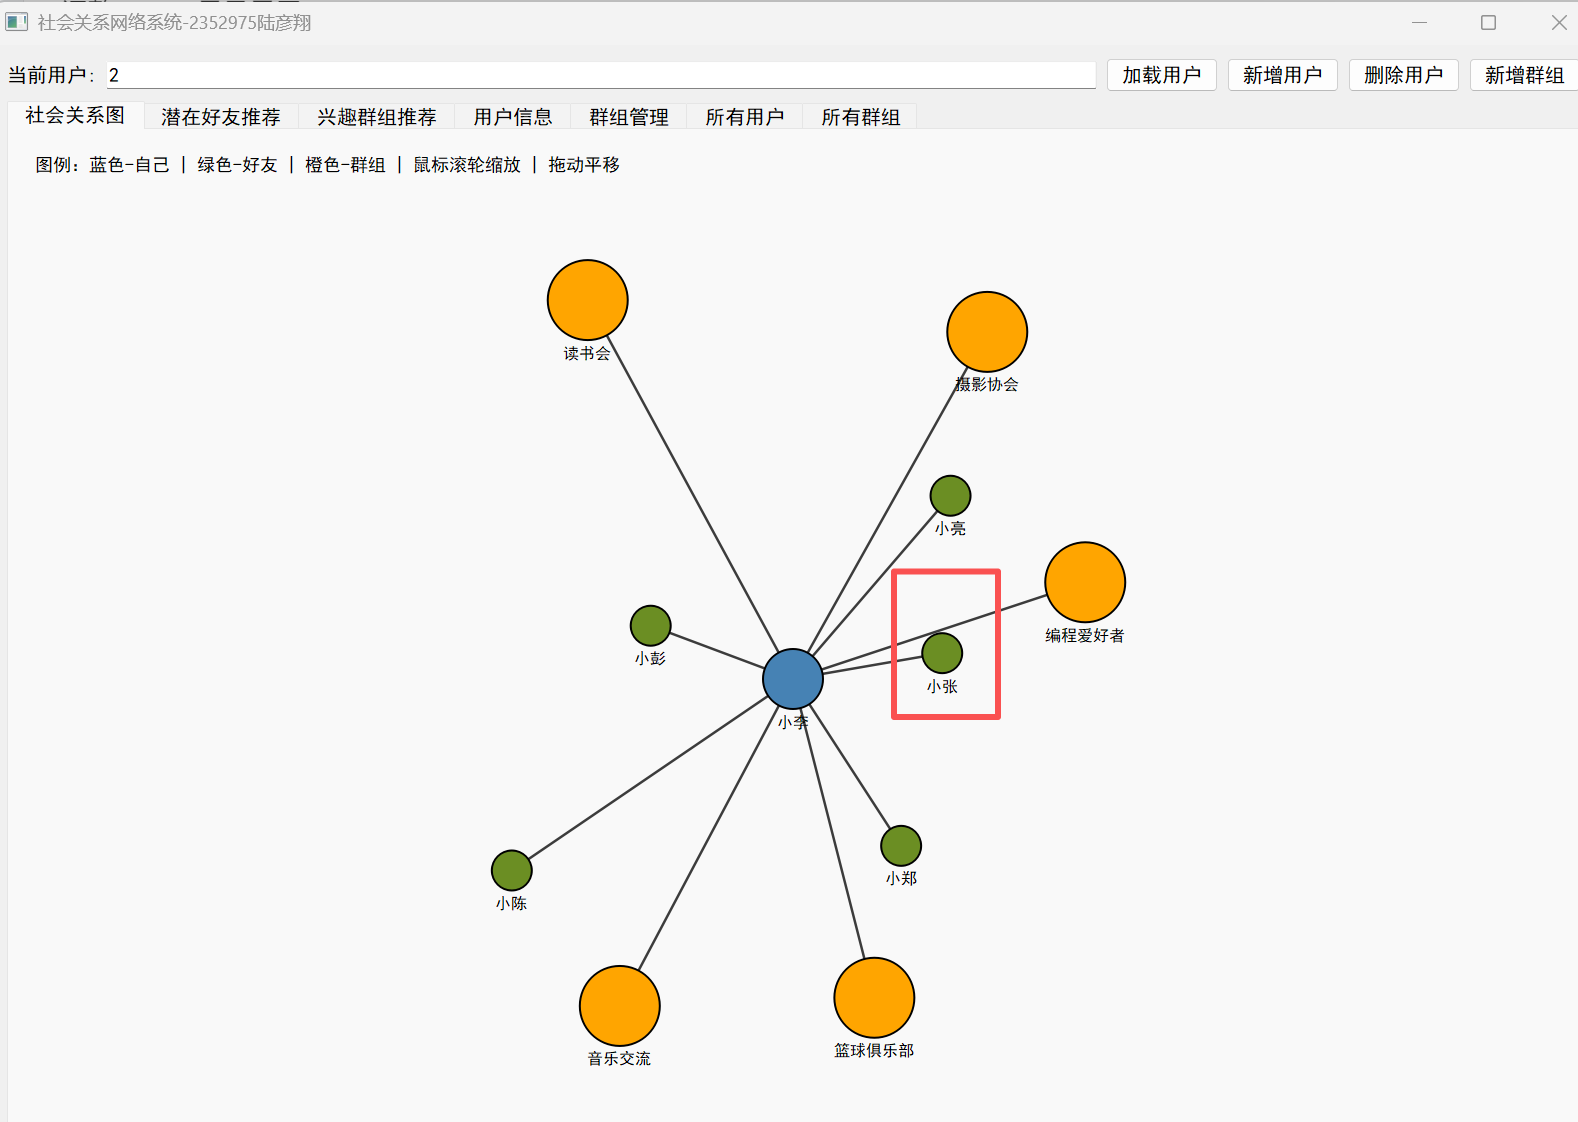
\includegraphics[width=0.5\textwidth]{pt2-19.png}
    \caption{社交关系图发生更新}
\end{figure}

删除好友时提供删除确认,防止误删。

\begin{figure}[H]
    \centering
    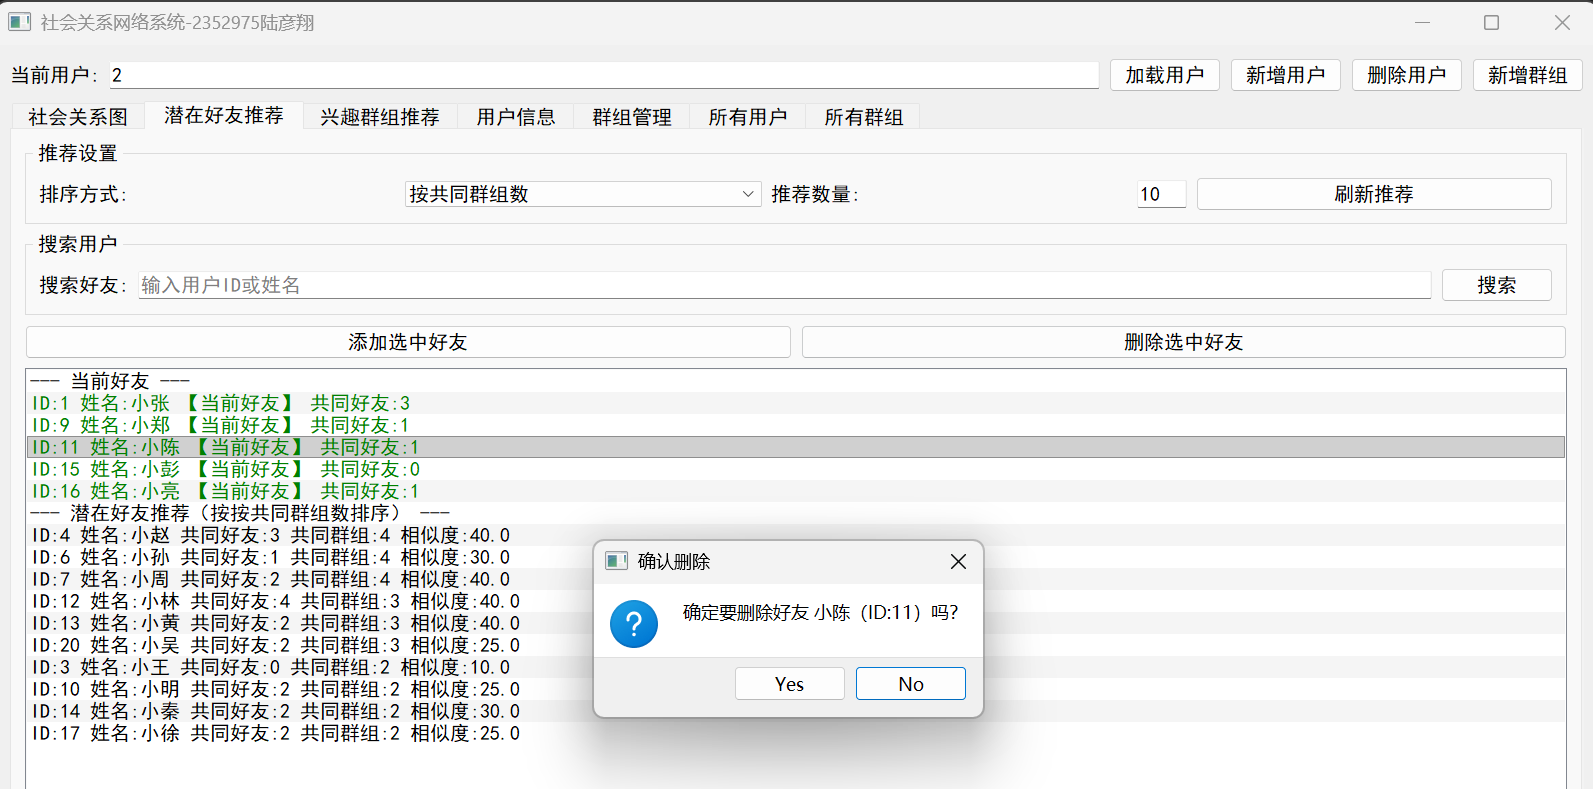
\includegraphics[width=0.5\textwidth]{pt2-20.png}
    \caption{删除好友确认}
\end{figure}

\begin{figure}[H]
    \centering
    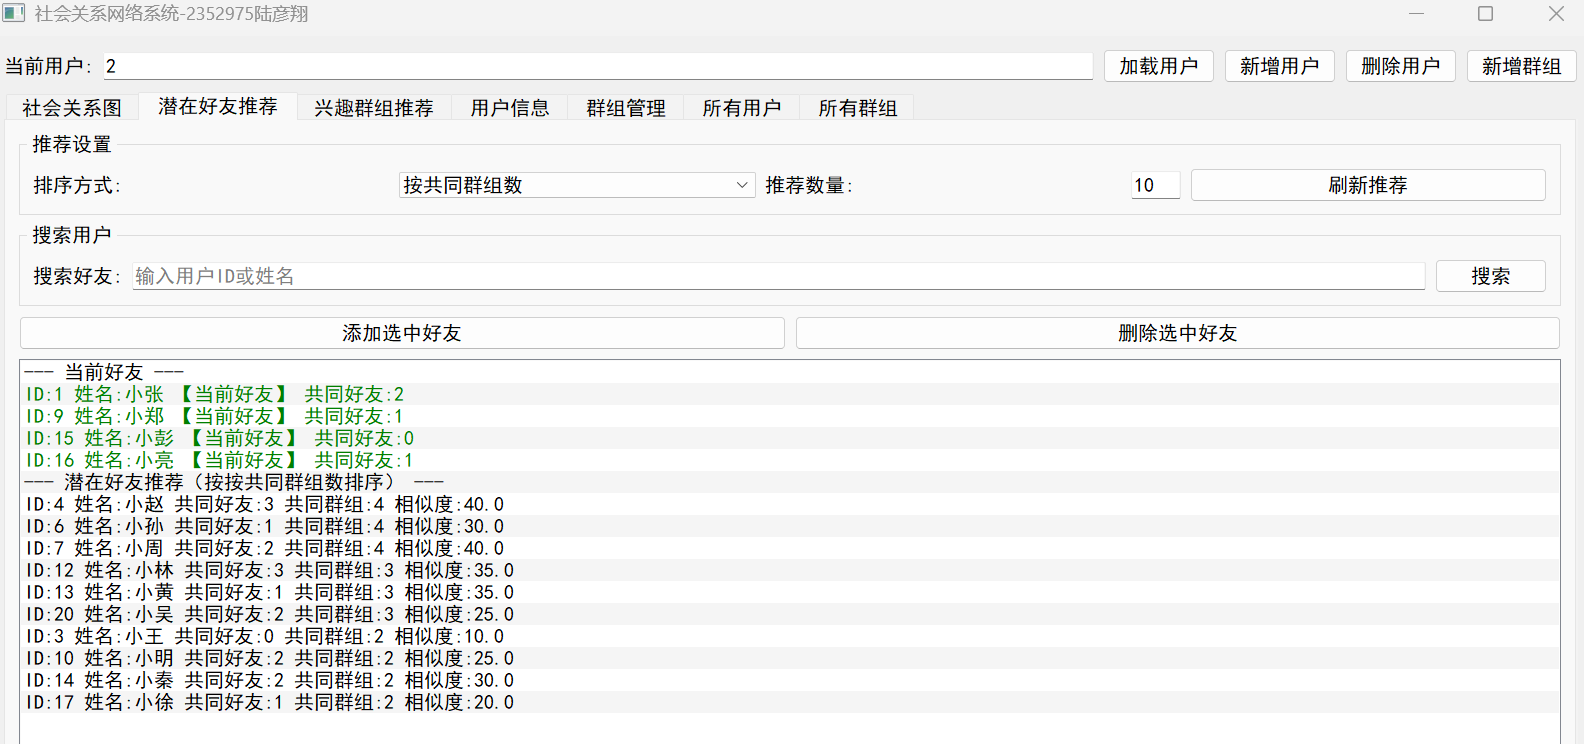
\includegraphics[width=0.5\textwidth]{pt2-23.png}
    \caption{确认删除}
\end{figure}

面对异常情况同样有处理,例如添加已经添加过的好友或者对未添加的人删除好友。

\begin{figure}[H]
    \centering
    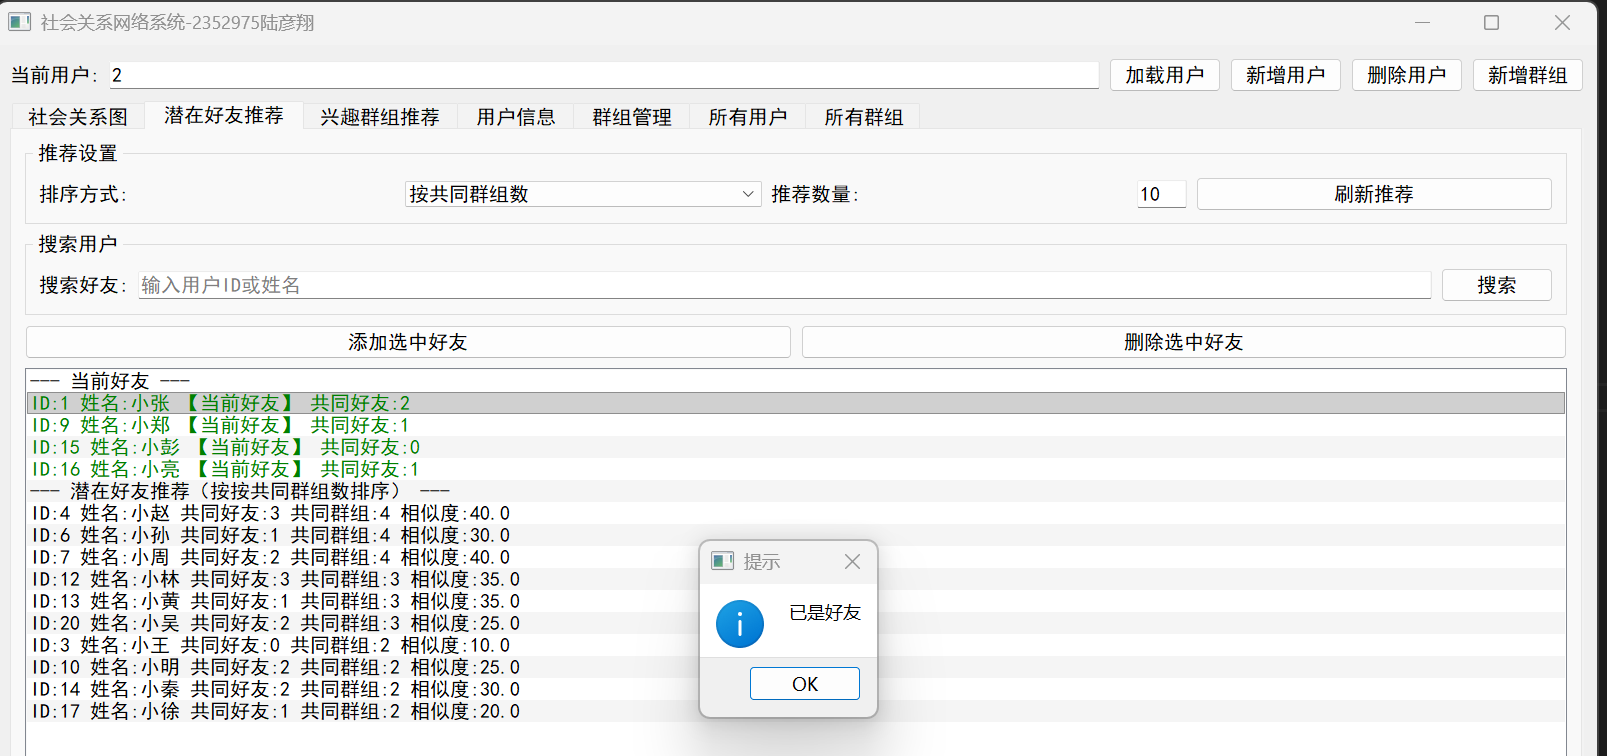
\includegraphics[width=0.5\textwidth]{pt2-21.png}
    \caption{添加已经添加过的好友}
\end{figure}

\begin{figure}[H]
    \centering
    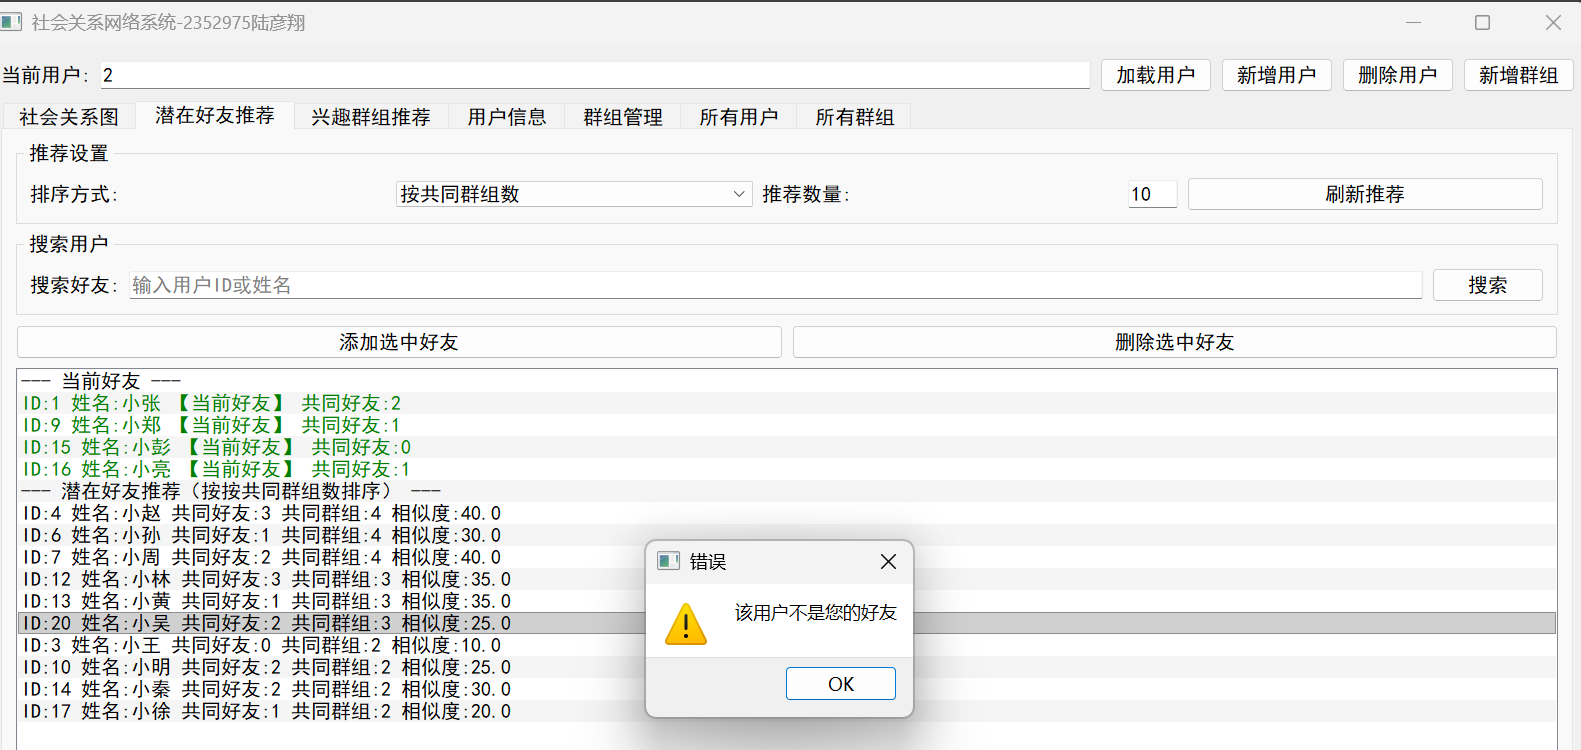
\includegraphics[width=0.5\textwidth]{pt2-22.png}
    \caption{删除未添加的人}
\end{figure}

在兴趣群组推荐中同样可以设定推荐个数并进行群组加入,但是对于没有匹配度的情况不会进行推荐。

\begin{figure}[H]
    \centering
    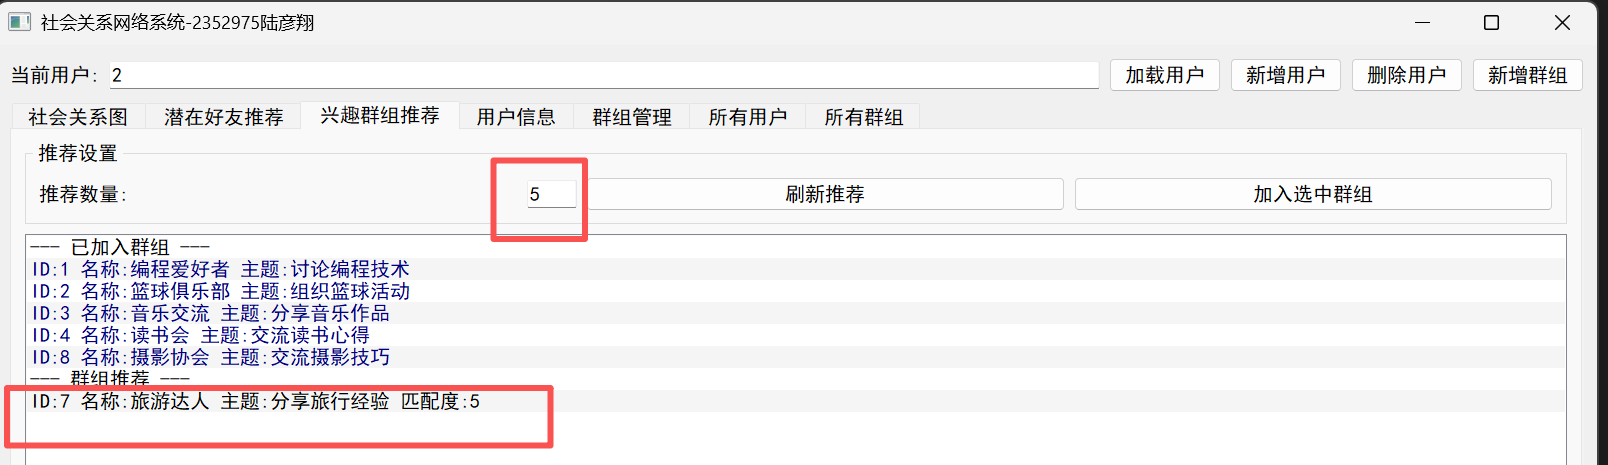
\includegraphics[width=0.5\textwidth]{pt2-24.png}
    \caption{兴趣群组推荐}
\end{figure}

\begin{figure}[H]
    \centering
    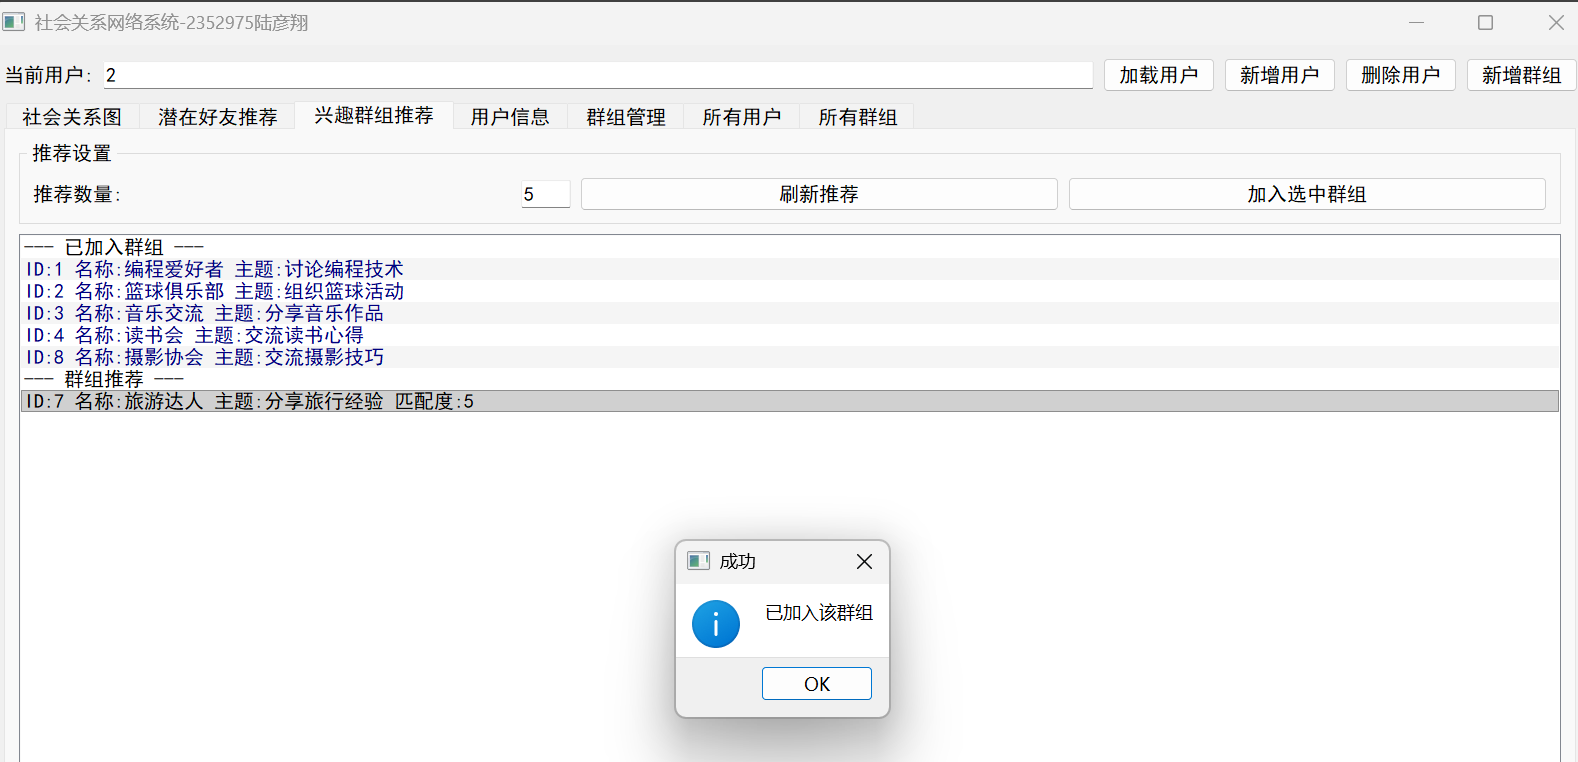
\includegraphics[width=0.5\textwidth]{pt2-25.png}
    \caption{加入选中群组}
\end{figure}

\begin{figure}[H]
    \centering
    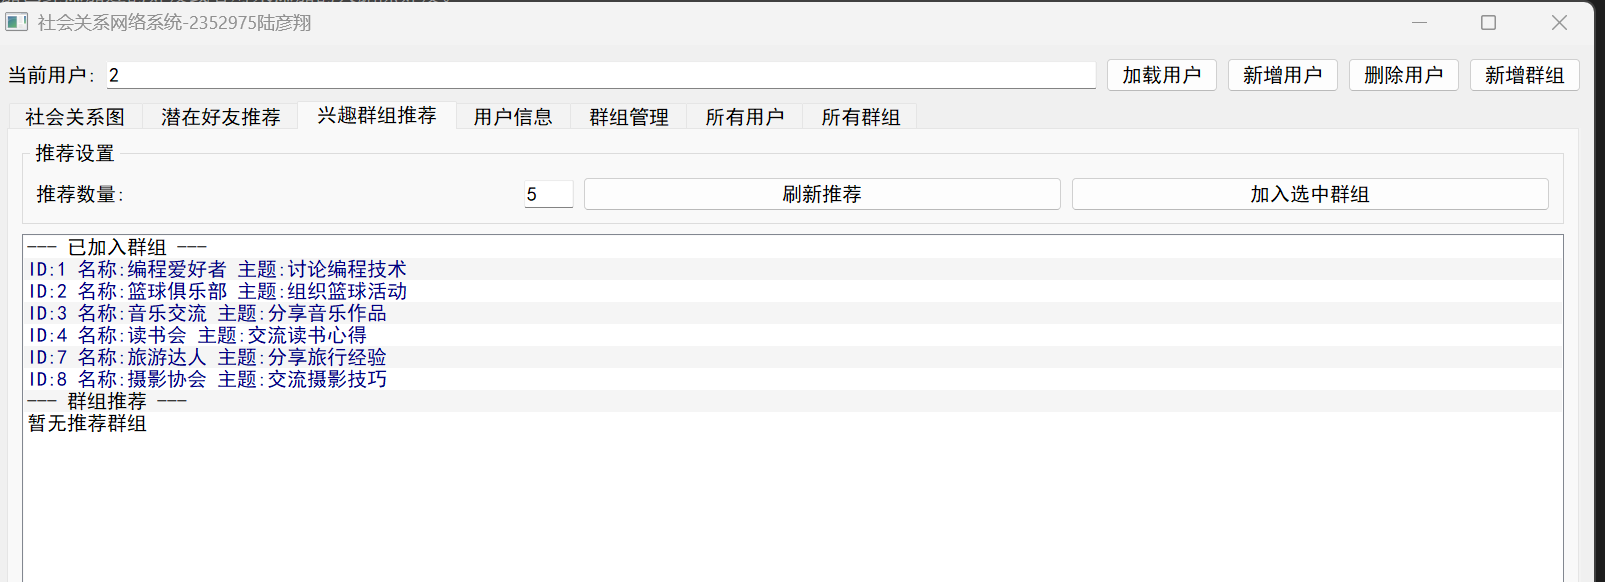
\includegraphics[width=0.5\textwidth]{pt2-26.png}
    \caption{群组推荐更新}
\end{figure}

\begin{figure}[H]
    \centering
    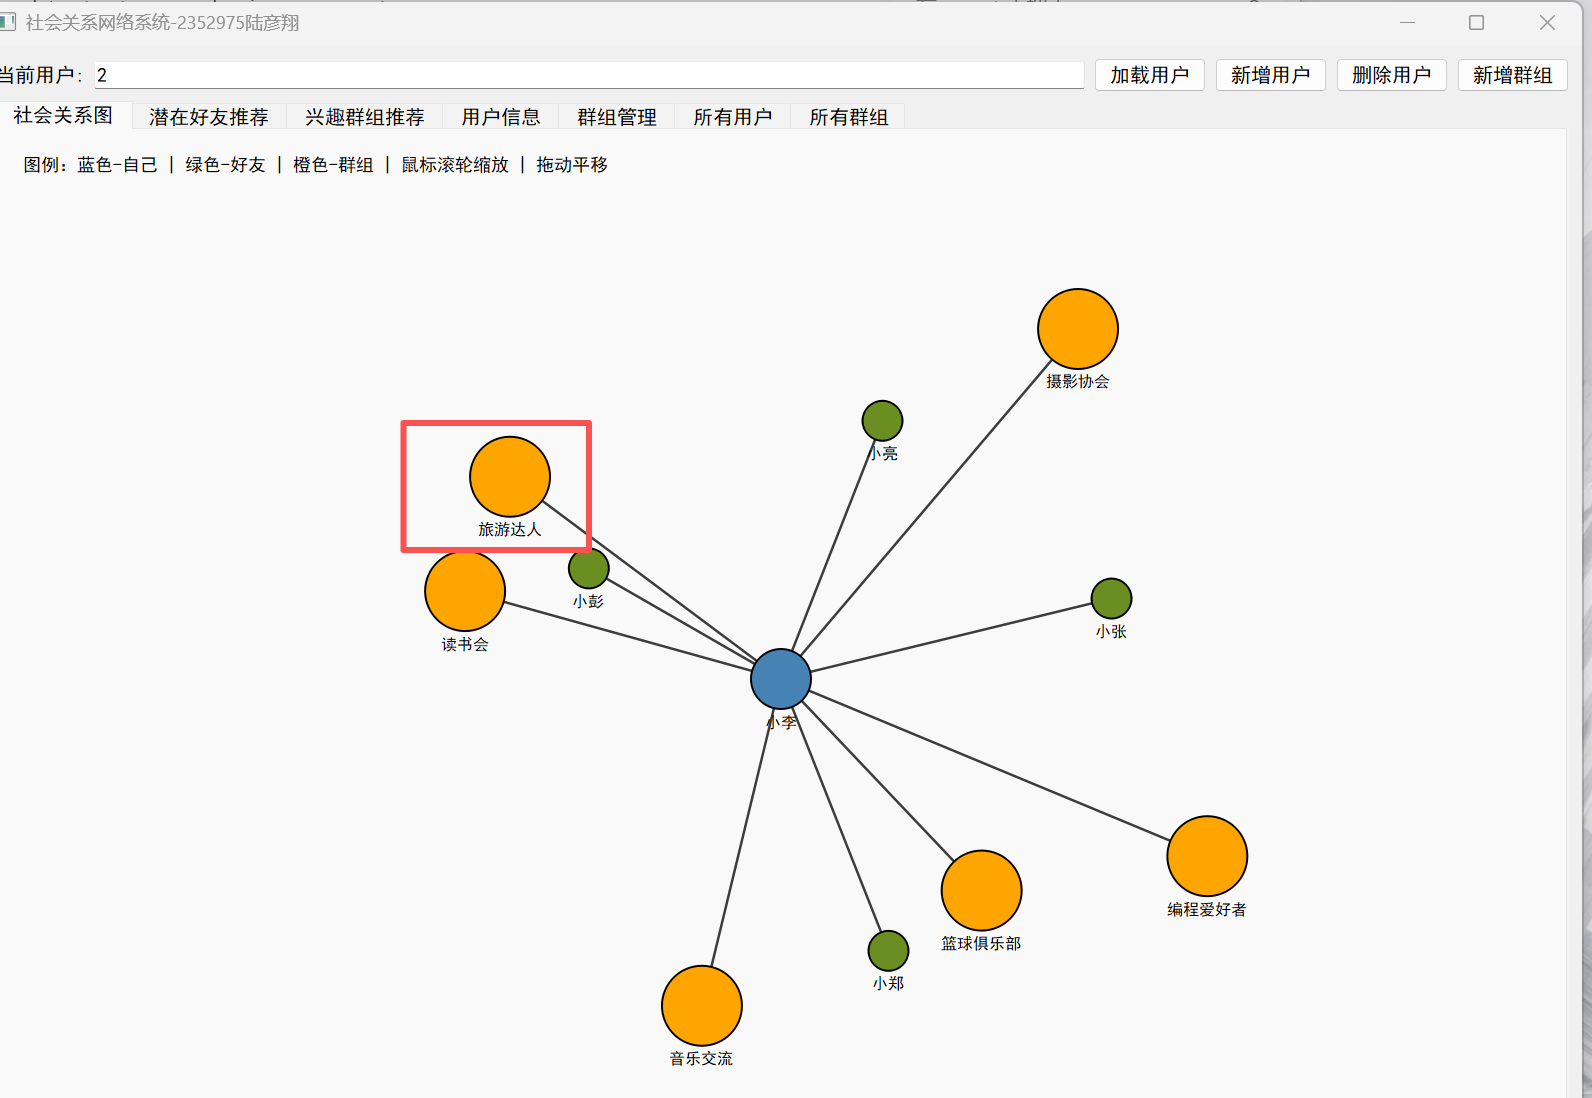
\includegraphics[width=0.5\textwidth]{pt2-27.png}
    \caption{社交关系图更新}
\end{figure}

可以在群组中加载制定群组并进行群组的退出

\begin{figure}[H]
    \centering
    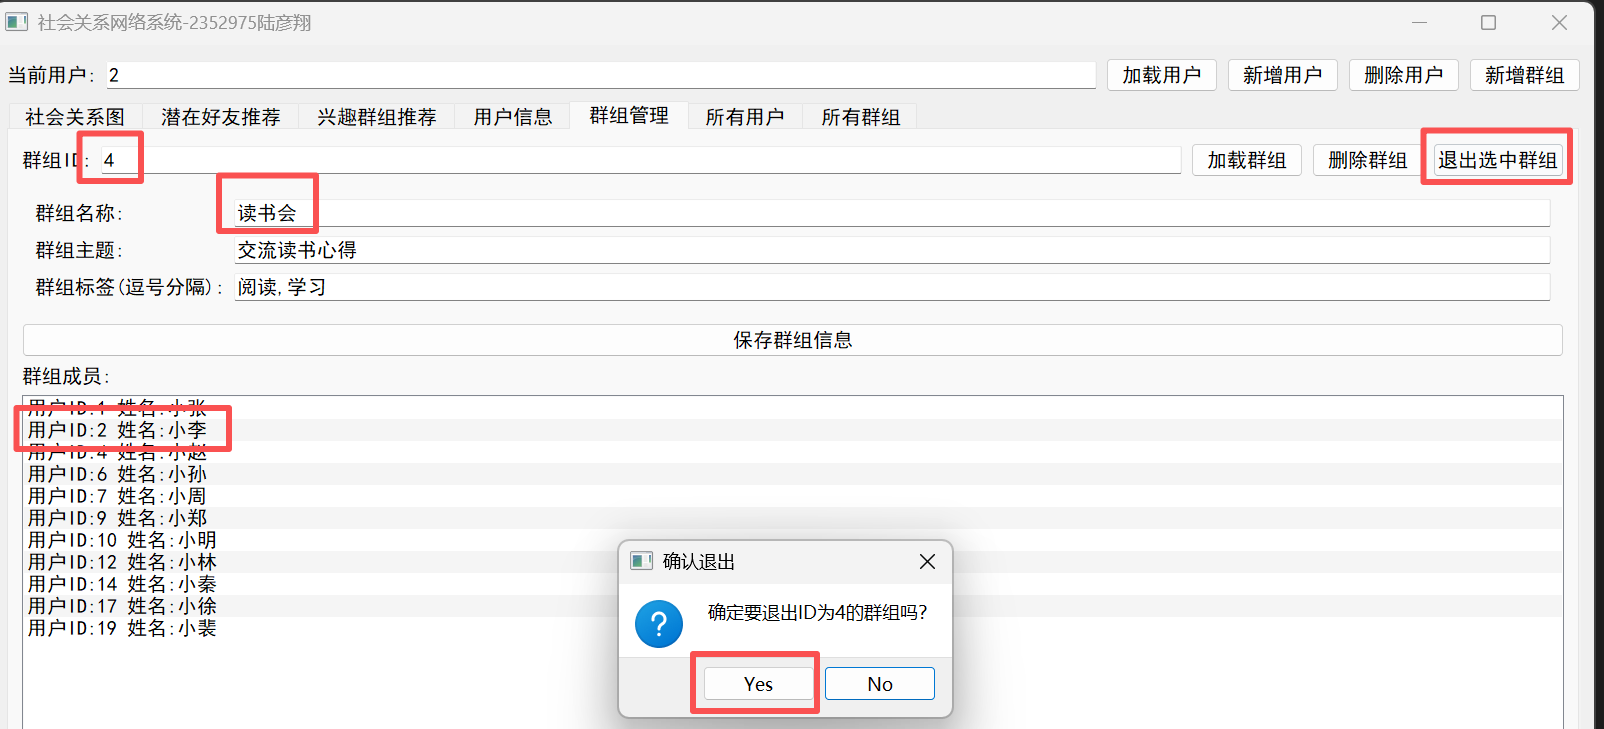
\includegraphics[width=0.5\textwidth]{pt2-28.png}
    \caption{退出选定群组}
\end{figure}

\begin{figure}[H]
    \centering
    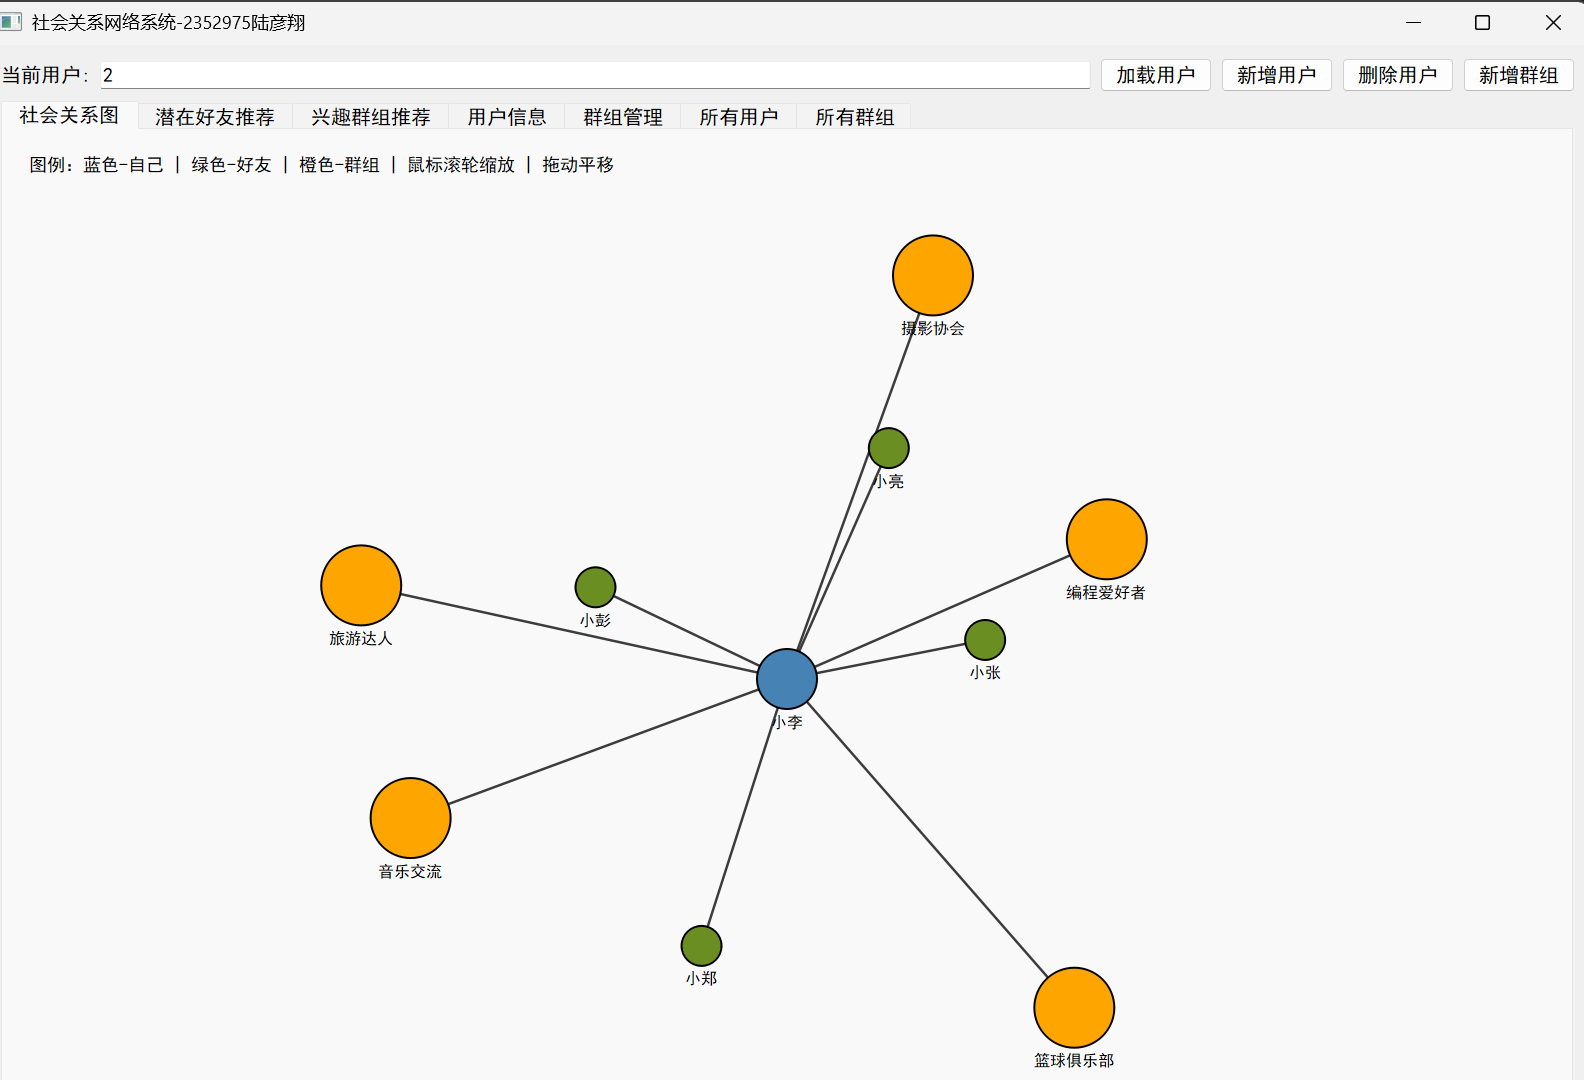
\includegraphics[width=0.5\textwidth]{pt2-29.png}
    \caption{社交关系图更新}
\end{figure}

\begin{figure}[H]
    \centering
    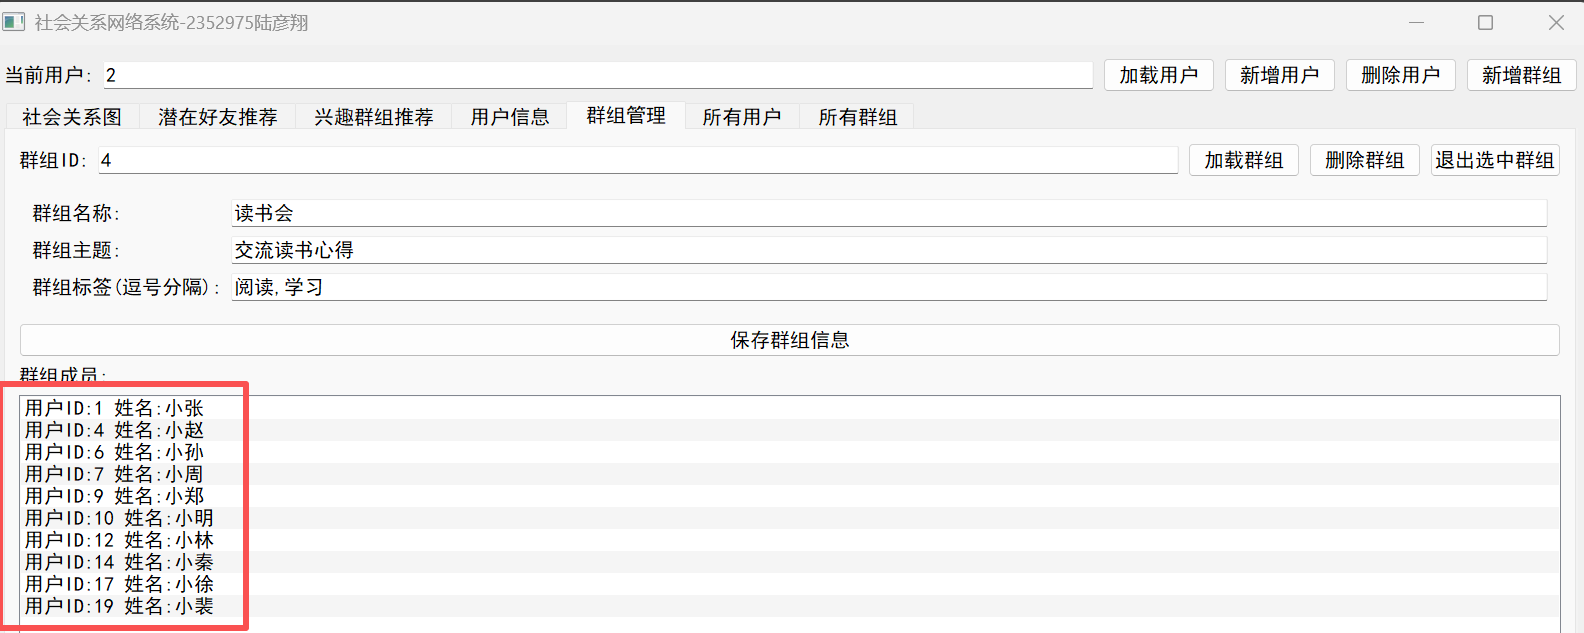
\includegraphics[width=0.5\textwidth]{pt2-30.png}
    \caption{群组用户信息变更}
\end{figure}

在群组内容中,如果直接加载一个不存在的群组,也会给出报错信息并保留当前控制对象

\begin{figure}[H]
    \centering
    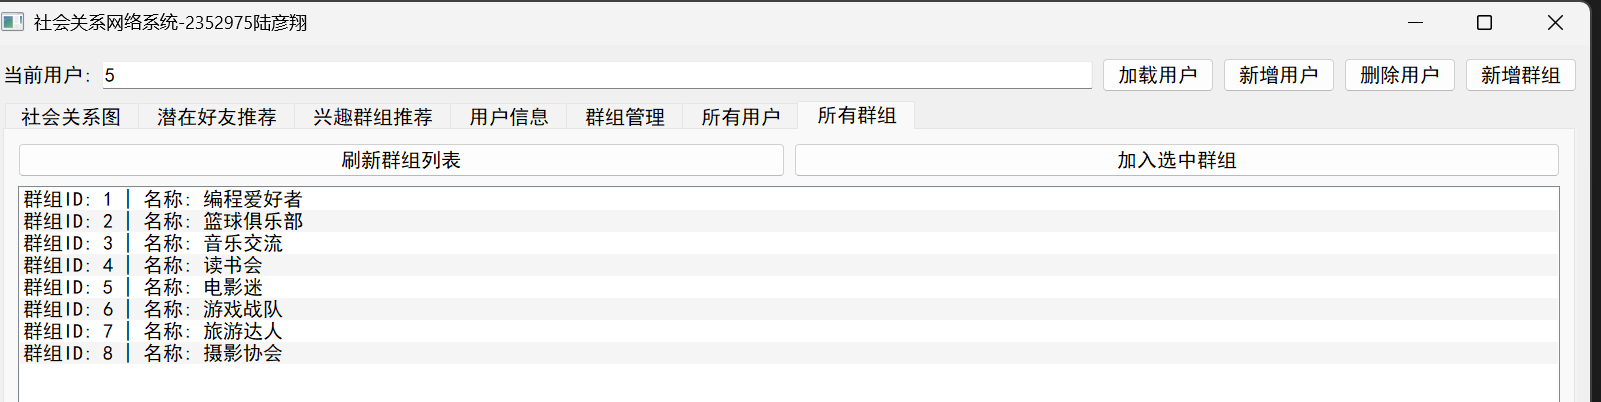
\includegraphics[width=0.5\textwidth]{pt2-31.png}
    \caption{当前所有群组}
\end{figure}

\begin{figure}[H]
    \centering
    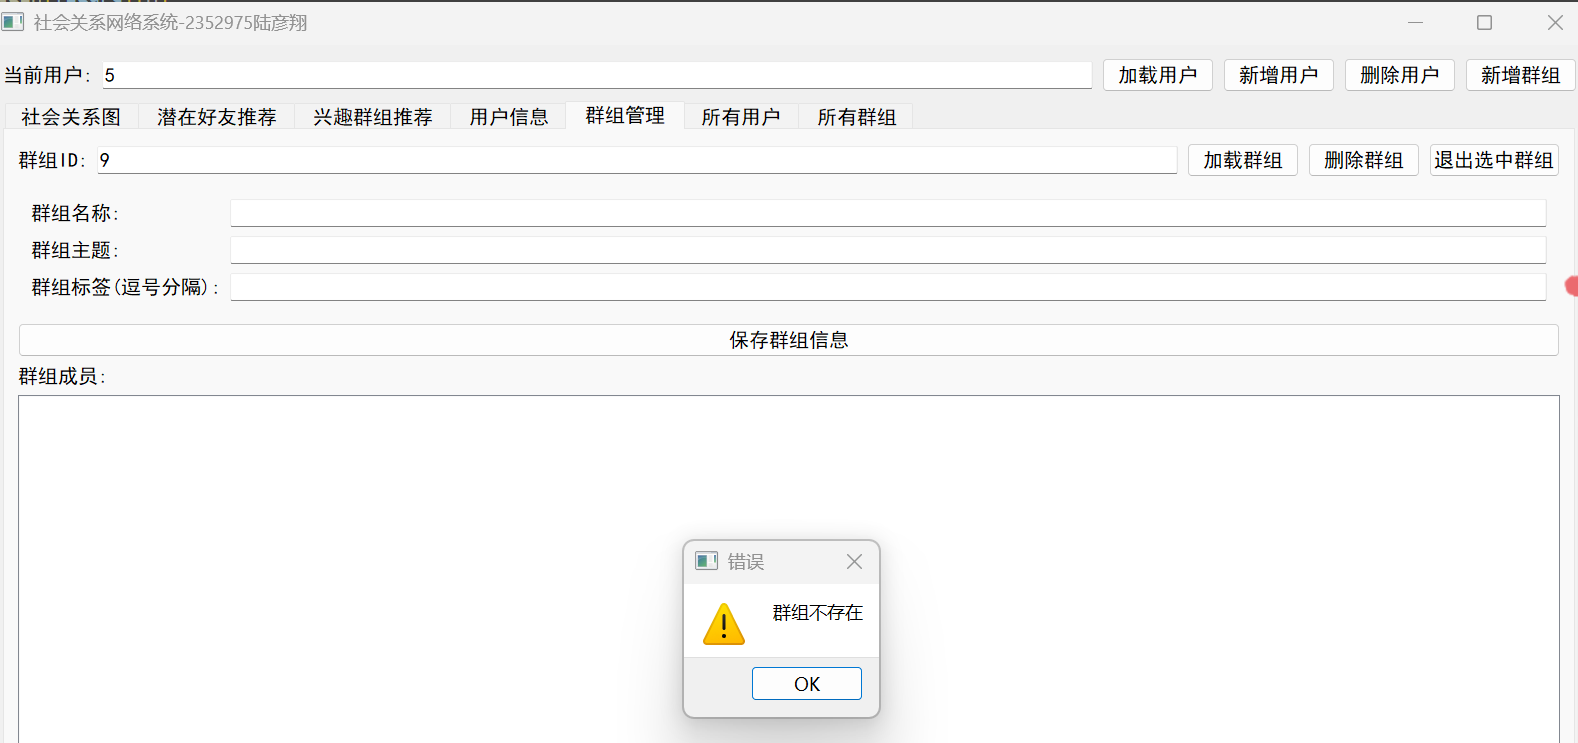
\includegraphics[width=0.5\textwidth]{pt2-32.png}
    \caption{加载不存在的群组}
\end{figure}

在群组管理中可以查看相关信息,并且进行内容的修改。

\begin{figure}[H]
    \centering
    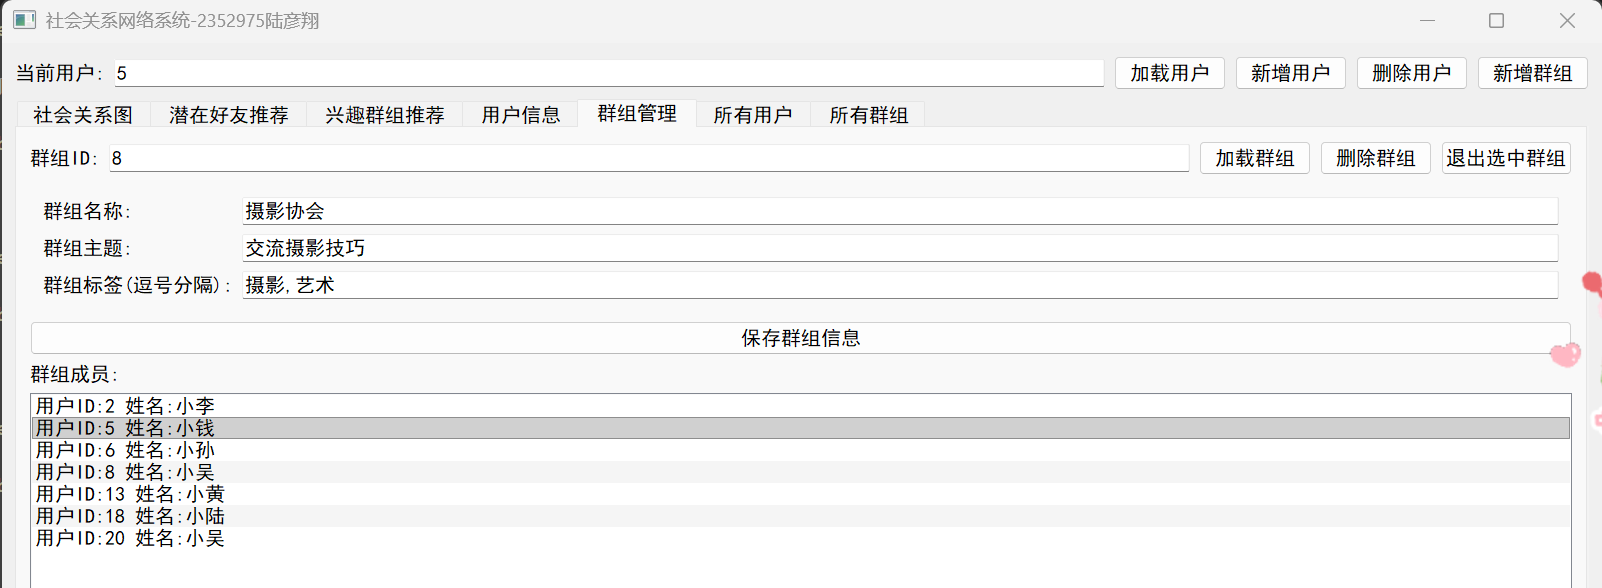
\includegraphics[width=0.5\textwidth]{pt2-33.png}
    \caption{当前群组信息}
\end{figure}

\begin{figure}[H]
    \centering
    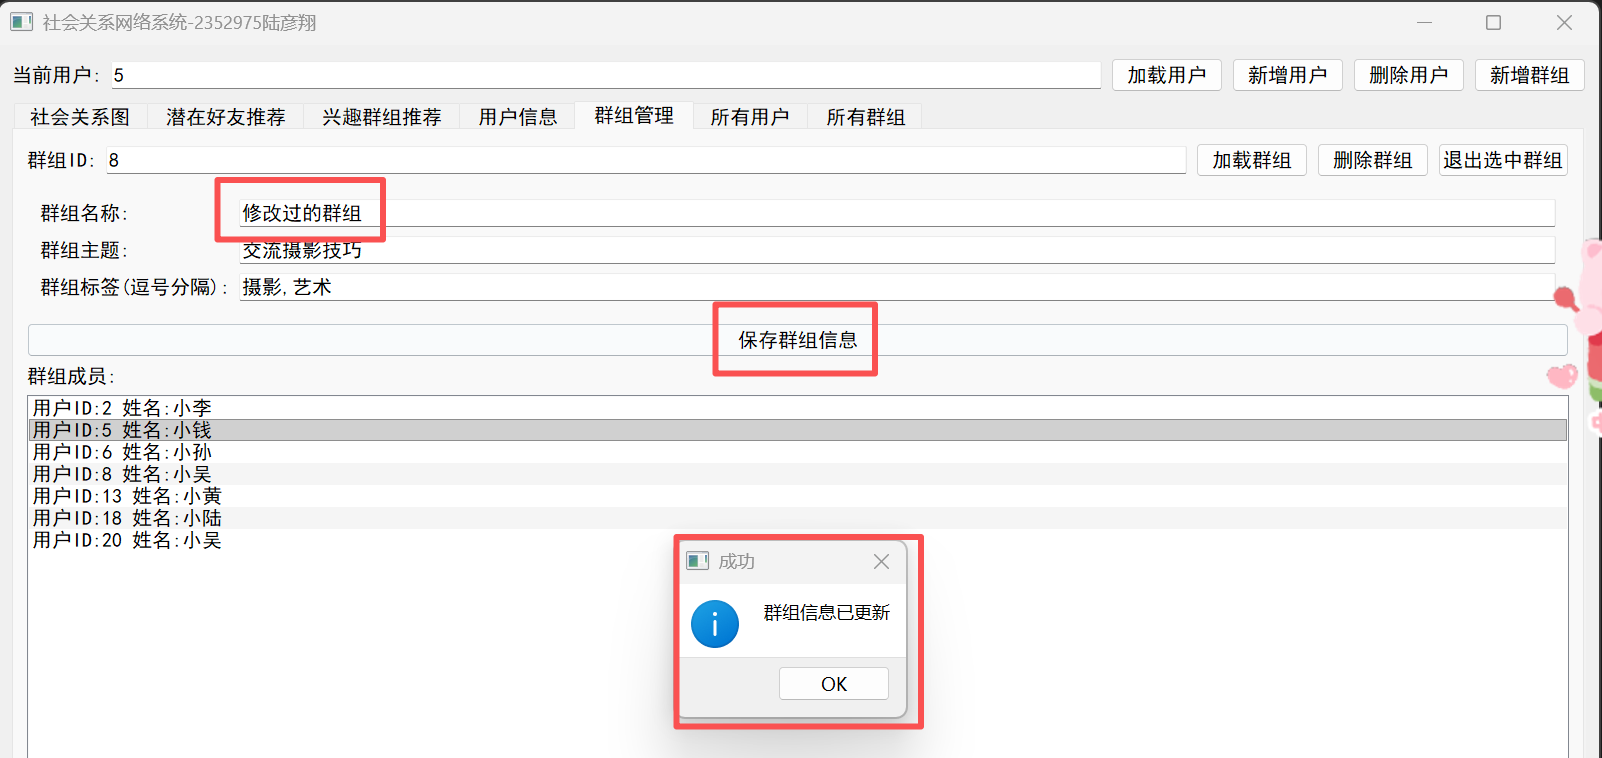
\includegraphics[width=0.5\textwidth]{pt2-34.png}
    \caption{群组信息修改}
\end{figure}

在所有群组中,点击刷新群组,可以发现信息被修改。

\begin{figure}[H]
    \centering
    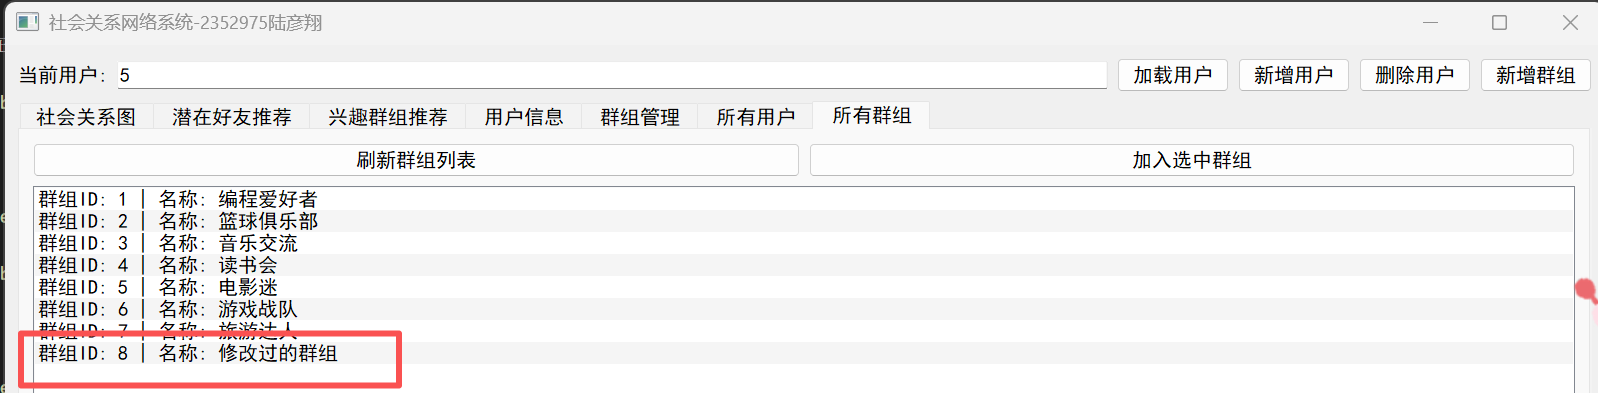
\includegraphics[width=0.5\textwidth]{pt2-35.png}
    \caption{在所有群组中可以发现信息被修改}
\end{figure}

我们重新加载这个群组ID为5的用户“小钱”并观察其社交网络,发现也随之更新

\begin{figure}[H]
    \centering
    \includegraphics[width=0.5\textwidth]{pt2-36.png}
    \caption{群组成员社交网络变更}
\end{figure}

\begin{figure}[H]
    \centering
    \includegraphics[width=0.5\textwidth]{pt2-37.png}
    \caption{群组推荐中信息也发生变更}
\end{figure}

点击删除群组触发确认操作,点击yes即可删除。

\begin{figure}[H]
    \centering
    \includegraphics[width=0.5\textwidth]{pt2-38.png}
    \caption{群组删除}
\end{figure}

\begin{figure}[H]
    \centering
    \includegraphics[width=0.5\textwidth]{pt2-39.png}
    \caption{群组信息被修改}
\end{figure}

在其他部分中也会 发生修改,因为和上面内容相似所以不再进行贴图展示。

成员信息也可以进行在成员界面中进行修改。

\begin{figure}[H]
    \centering
    \includegraphics[width=0.5\textwidth]{pt2-40.png}
    \caption{ID为5的用户的当前信息}
\end{figure}

我们以改变最直观的用户姓名为例,把“小钱”更名为“钱多多”,并点击保存按钮。

\begin{figure}[H]
    \centering
    \includegraphics[width=0.5\textwidth]{pt2-41.png}
    \caption{修改用户信息}
\end{figure}

在全体用户列表中刷新,发现用户信息更改。

\begin{figure}[H]
    \centering
    \includegraphics[width=0.5\textwidth]{pt2-42.png}
    \caption{全体列表中用户信息更改}
\end{figure}

在关系网中加载,发现用户信息更改。

\begin{figure}[H]
    \centering
    \includegraphics[width=0.5\textwidth]{pt2-43.png}
    \caption{关系网更改}
\end{figure}

\begin{figure}[H]
    \centering
    \includegraphics[width=0.5\textwidth]{pt2-44.png}
    \caption{加入的群组中信息也随之修改}
\end{figure}

通过输入框右侧的删除按钮可以删除用户

\begin{figure}[H]
    \centering
    \includegraphics[width=0.5\textwidth]{pt2-45.png}
    \caption{删除用户会提示连带所有关系}
\end{figure}

\begin{figure}[H]
    \centering
    \includegraphics[width=0.5\textwidth]{pt2-46.png}
    \caption{在全体用户中发现少了一个用户}
\end{figure}

下一次新增用户时,会优先利用回收的ID。

\begin{figure}[H]
    \centering
    \includegraphics[width=0.5\textwidth]{pt2-47.png}
    \caption{新增用户}
\end{figure}

\begin{figure}[H]
    \centering
    \includegraphics[width=0.5\textwidth]{pt2-51.png}
    \caption{预设用户地区}
\end{figure}

\begin{figure}[H]
    \centering
    \includegraphics[width=0.5\textwidth]{pt2-48.png}
    \caption{在全体用户中检查新用户}
\end{figure}

\begin{figure}[H]
    \centering
    \includegraphics[width=0.5\textwidth]{pt2-49.png}
    \caption{在全体群组管理中加入群组}
\end{figure}

\begin{figure}[H]
    \centering
    \includegraphics[width=0.5\textwidth]{pt2-50.png}
    \caption{关系图更新}
\end{figure}

\noindent\textbf{软件稳定性分析}

在项目设计中,我充分考虑了错误情况,无论是加载错误ID,群组还是加入已经加入的群组或者删除非好友用户等具有错误可能得操作,都进行了提示。同时为了防止用户的错误操作,还在进行删除操作时都进行了确认设置,进一步提升了系统的安全性与稳定性。

\section{实践总结}

\subsection{所做的工作}

在本次实验过程中,我实现了二叉树图形化操作界面以及社交关系网络的设计,基于MVC设计模式构建了完整的系统架构,通过创建多个类来实现模块化编程。在两个编程任务中我都使用了PyQt5来开发完整的用户交互界面,同时实现了两个项目社交关系可视化组件的缩放和平移支持。

在人际关系网络的设计中,我还尝试结合数据库的知识,实现了完善的ID重复利用机制,提高系统资源的利用效率。

\subsection{总结与收获}

在本次的两个项目设计工程中,我了解了PyQt5图形化界面的开发框架,学会使用信号槽机制,事件处理,自定义组件等特性。同时,我还进一步掌握了面向对象编程思想,在代码完成过程中进一步学会了封装代码并了解了他的优势。在算法设计过程中,我也尝试自行设计推荐方法,来为用户做出更准确的推荐。

这次代码实践也让我学会乐乐大型项目的架构设计方法,掌握了模块化开发和代码组织技巧,更加注重代码的可读性和可维护性,

我也学习了MVC设计模式,尝试进行系统层次的划分,提高了代码维护意识。

\subsection{个人体会}

这个项目不仅让我更好的掌握了之前学习到的数据结构知识,也培养了我的自主学习能力,通过查阅资料自行学习用户交互界面的设计。同时我还体会到了将项目任务划分的重要性。

总的来说,这个项目不仅让我获得了技术上的提升,还培养了我的自学、项目管理、问题解决和时间管理能力。希望在本次课程设计中获得的经验能够让我更好的掌握大型项目的编写方式。 


\end{document}